%% HINWEIS: Die Kombi-Datei wird parallel zur _ger-Version gepflegt.
%% Master: _ger-Version. Bei Aenderungen immer _ger zuerst, dann Kombi.
%% Stand: 2026-03-17 Sync mit _ger v2 (Review-Runden 1-3)
%% =============================================================================
%% KI_Elite_v2_kombi.tex
%% Was denkt die KI-Elite? Eine LLM-gestuetzte Weltbild-Rekonstruktion
%% der 100 einflussreichsten Akteure der kuenstlichen Intelligenz (2010--2026)
%% Autor: Lukas Geiger, Unabhaengiger Forscher, Bernau
%% Companion Paper: SWR_v1_ger.tex (Synthetische Weltbild-Rekonstruktion)
%% =============================================================================
\documentclass[12pt,a4paper]{article}

%% --- Kodierung und Sprache ---------------------------------------------------
\usepackage[utf8]{inputenc}
\usepackage[T1]{fontenc}
\usepackage[ngerman,english]{babel}

%% --- Schrift: Times New Roman ------------------------------------------------
\usepackage{mathptmx}
\usepackage[scaled=0.92]{helvet}

%% --- Seitenlayout ------------------------------------------------------------
\usepackage[left=2.5cm, right=2.5cm, top=2.5cm, bottom=2.5cm]{geometry}

%% --- Zeilenabstand: 1,5 -----------------------------------------------------
\usepackage{setspace}
\onehalfspacing

%% --- Ueberschriften serifenlos -----------------------------------------------
\usepackage{titlesec}
\titleformat{\section}
  {\normalfont\Large\bfseries\sffamily}{\thesection.}{0.5em}{}
\titleformat{\subsection}
  {\normalfont\large\bfseries\sffamily}{\thesubsection}{0.5em}{}
\titleformat{\subsubsection}
  {\normalfont\normalsize\bfseries\sffamily}{\thesubsubsection}{0.5em}{}

%% --- Zitation: natbib Autor-Jahr ---------------------------------------------
\usepackage[round,authoryear,semicolon]{natbib}
\bibliographystyle{plainnat}

%% --- Pakete ------------------------------------------------------------------
\usepackage{graphicx}
\graphicspath{{../_results/figures/}}
\usepackage{booktabs}
\usepackage{array}
\usepackage{tabularx}
\usepackage{longtable}
\usepackage{amsmath,amssymb}
\usepackage{enumitem}
\usepackage{xcolor}
\usepackage{url}
\usepackage[german=quotes]{csquotes}
\usepackage[breaklinks=true]{hyperref}
\hypersetup{
  colorlinks  = true,
  linkcolor   = black,
  citecolor   = blue!60!black,
  urlcolor    = blue!70!black,
  pdfauthor   = {Lukas Geiger},
  pdftitle    = {Worldview Reconstruction of the AI Elite: An LLM-Assisted Analysis (2010--2026)},
  pdfsubject  = {Computational Social Science},
}

%% --- Titelblock --------------------------------------------------------------
\title{%
  \sffamily\bfseries
  Worldview Reconstruction of the AI Elite:\\[0.3em]
  \large An LLM-Assisted Analysis of the 100 Most Influential\\
  Actors in Artificial Intelligence (2010--2026)%
}

\author{%
  Lukas Geiger\thanks{Corresponding author: Lukas Geiger, Bernau, Germany. ORCID: \url{https://orcid.org/0009-0005-7296-1534}}\\[0.3em]
  \small Independent Researcher, Bernau, Germany
}

\date{March 2026}

%% =============================================================================
\begin{document}

% Language: English (main)

%% =============================================================================

\maketitle
\thispagestyle{empty}

%% --- Abstract ----------------------------------------------------------------
\begin{abstract}
\noindent
This study is the first to systematically reconstruct the collective worldview of the 100 most influential figures in artificial intelligence (AI elite) for the period 2010 to 2026. Methodologically, it develops and applies synthetic worldview reconstruction (SWR) -- an LLM-assisted procedure that extracts coherent belief systems from 3,132 data points (1,738 public statements, 1,394 observable actions) using 51--56 synthesis units, 12 worldview dimensions, and 6 complementary operationalizations (cf.\ the companion paper \citealt{Geiger2026SWR} for the methodological foundations). Six research questions structure the analysis: RQ1~(Worldview) reveals a ``technological messianism with ambivalence structure'' (Avg~7.1 collective, 7.7 Top~10). RQ2~(Change) documents the transition from utopian techno-optimism to tragic acceleration compulsion; posthumanism declines markedly ($-2.4$/decade, $R^2 = 0.63$; descriptive OLS, not inferential statistics). RQ3~(Congruence) uncovers a systematic say-do gap; largest discrepancy in egalitarianism ($\Delta = -3$). RQ4~(Clusters) identifies four worldview types: Architect, Guardian, Innovator, Liberator. RQ5~(Difference) names the strongest predictors: stance ($\Delta$~1.7), role ($\Delta$~1.5), gender ($\Delta$~1.2). RQ6~(Power) reveals a power-moderation paradox: the most powerful type is the most extreme; the most moderate is the least powerful.

\medskip
\noindent\textbf{Keywords:} AI elite, worldview, transhumanism, large language models, Silicon Valley, ideology analysis
\end{abstract}

\newpage
\setcounter{page}{1}

%% =============================================================================
%% 1. INTRODUCTION
%% =============================================================================
\section{Introduction}
\label{sec:einleitung}

\subsection{Lead-in and Relevance}
\label{sec:einleitung:relevanz}

A handful of people are shaping a technology that affects billions. Over the past one and a half decades, the development of artificial intelligence has evolved from an academic niche topic into a civilizational crossroads. Large language models generate texts, images, and code; autonomous systems make decisions in medicine, law, and finance; and leading AI laboratories openly speak of creating artificial general intelligence in the foreseeable future \citep{OpenAI2023Charter, AnthropicCoreViews2023, Bengio2024}. What is easily overlooked: behind these technological trajectories stand concrete individuals -- founders, research directors, investors, CEOs -- whose individual and collective beliefs about the nature of humanity, the purpose of progress, and the distribution of risk and power flow into the architecture of the systems they build.

\citet{Lessig1999} coined the formula ``code is law'': software architecture regulates behavior no less effectively than laws, but without democratic legitimation. This insight can be radicalized for the current AI development: not only the code itself, but already the \emph{worldviews} of the developers become algorithms. Those who believe that information freedom is an absolute value will build open-source models. Those convinced that an uncontrolled superintelligence threatens humanity will pursue alignment and closed systems. The worldviews of the AI elite are thus not merely private opinions; they are \emph{generative structures} that translate into design decisions, corporate strategies, and political positions -- and through these channels shape the lives of billions.

This creates a fundamental problem for democratic theory. A numerically tiny group makes decisions of society-wide consequence without possessing a democratic mandate. \citet{Crawford2021} has described this as an ``Atlas of AI'': the planetary power structures behind AI systems remain largely invisible. \citet{Zuboff2019} analyzes how the extraction of behavioral data leads to a new economic logic (``Surveillance Capitalism'') that undermines democratic control. \citet{Couldry2019} coin the term ``Data Colonialism'': the exploitation of human life as a data resource. \citet{Whittaker2021} analyzes the concentration of power in AI research and its ``steep costs'' for society. Their beliefs shape these decisions in ways that are largely beyond public control \citep{Floridi2019, Floridi2023}. If democracies presuppose informed citizens, then the systematic reconstruction of the worldviews of those who shape the most powerful technology of the 21st century is not merely an academic concern but a prerequisite for informed public deliberation.


\subsection{Research Gap}
\label{sec:einleitung:luecke}

The scholarly engagement with the belief systems of the AI industry has produced various approaches. At the level of ideology critique, \citet{BarbCam1996} described the ``Californian Ideology''; \citet{Morozov2013} elaborated the tendency toward solutionism; \citet{Daub2020} analyzed the rhetorical and ideological patterns of Silicon Valley as a cultural phenomenon. From transhumanism research, philosophical analyses exist \citep{Bostrom2005, MoreVitaMore2013, Coeckelbergh2020}, which, however, primarily address intellectual history rather than the empirical distribution of these beliefs.

What is still \emph{missing} in this research field is a systematic, data-driven analysis of the \emph{entire} AI elite as a collective. No study examines, as far as the author is aware, the following questions in an empirically systematic way: How do the worldviews of leading AI actors relate to each other? Do they form coherent types? How have these worldviews changed over the period 2010 to 2026? And do public beliefs align with actual behavior?

Beyond this empirical gap, there is a \emph{methodological} gap. No established method exists for the systematic reconstruction of worldviews from public statements at scale. Classical qualitative methods do not scale; standardized surveys require access to respondents; quantitative text-mining approaches capture only surface patterns. The present study responds to this dual gap with a new approach -- synthetic worldview reconstruction (SWR) -- whose methodological foundations are set out in detail in a companion paper \citep{Geiger2026SWR}.


\subsection{Research Questions}
\label{sec:einleitung:fragen}

From the described research gap, six research questions are derived, arranged in a stepwise logic:

\begin{description}[style=nextline, leftmargin=1.5cm]
  \item[RQ1: WORLDVIEW (descriptive)] \emph{What does the AI elite think about itself, the world, and humanity?}
  \item[RQ2: CHANGE (longitudinal)] \emph{How has the worldview of the AI elite changed from 2010 to 2026?}
  \item[RQ3: CONGRUENCE (validating)] \emph{Do the AI elite's statements and actions align?}
  \item[RQ4: CLUSTERS (exploratory)] \emph{What worldview types exist within the AI elite, and who belongs where?}
  \item[RQ5: DIFFERENCE (comparative)] \emph{Which subgroups of the AI elite think differently from others?}
  \item[RQ6: POWER (normative)] \emph{Which worldview commands the most power and resources?}
\end{description}


\subsection{Contribution of the Study}
\label{sec:einleitung:beitrag}

The study makes a threefold contribution. \emph{Methodologically:} It applies synthetic worldview reconstruction (SWR; cf.\ companion paper \citealt{Geiger2026SWR}) for the first time to a large empirical dataset. \emph{Empirically:} It provides the first systematic worldview analysis of the AI elite as a collective, based on 3,132 data points spanning 16 years. \emph{Societally:} It creates a foundation for informed public deliberation by making transparent the implicit assumptions behind AI design decisions.


%% =============================================================================
%% 2. LITERATURE REVIEW
%% =============================================================================
\section{Literature Review}
\label{sec:forschungsstand}

The study situates itself at the intersection of four research traditions.

\subsection{Silicon Valley as Ideology}
\label{sec:forschungsstand:sv}

Critical engagement with the thinking of Silicon Valley has produced a rich literature since the mid-1990s. \citet{BarbCam1996} coined the term ``Californian Ideology'' -- the paradoxical fusion of libertarian individualism and techno-utopian optimism. \citet{Turner2006} traced the cultural-historical genealogy of this ideology and showed how the counterculture of the 1960s was transformed into digital utopianism. \citet{Daub2020} uncovered the philosophical deep structures: fragments from Heidegger, Ayn Rand, and Puritan predestination doctrine form a ``surprisingly narrow philosophical foundation.'' \citet{Morozov2013} described solutionism -- the default attitude of redefining complex social problems as technical challenges. \citet{TorresGebru2024} systematized these currents in the TESCREAL framework: Transhumanism, Extropianism, Singularitarianism, Cosmism, Rationalism, Effective Altruism, and Longtermism as an ``interconnected bundle.'' Additionally, \citet{Broussard2018} coined the term ``technochauvinism'' for a systematic critique.

Previous research has thus described the \emph{ideology} of Silicon Valley at various levels. What it has not achieved is a systematic empirical mapping of the \emph{concrete worldviews} of real actors.


\subsection{Transhumanism and AI Eschatology}
\label{sec:forschungsstand:transhumanismus}

\citet{Bostrom2014} defined the conceptual framework in which a significant part of the AI elite has since operated with \emph{Superintelligence}. In earlier work, \citet{Bostrom2005} systematized the intellectual-historical foundations of transhumanism. \citet{More2003} presented the founding document of extropianism with the ``Principles of Extropy.'' \citet{Kurzweil2005} popularized the tradition with the Singularity thesis. From a philosophical perspective, \citet{Habermas2001} formulated one of the most significant counter-positions: the technological manipulation of future persons undermines their autonomy.

The empirical question remains unresolved: Do real AI actors share these convictions? In what mixture, with what modifications, and in what distribution?


\subsection{Worldview Research and Sociology of Knowledge}
\label{sec:forschungsstand:wissenssoziologie}

\citet{Mannheim1929} founded the tradition of analyzing worldviews as social phenomena with his theorem of the ``situational determination of thought'' (\emph{Seinsgebundenheit des Denkens}). \citet{Weber1904} created with the ideal type a methodological tool central to the present study: the synthetic personas of the SWR can be understood as ideal types in the Weberian sense. \citet{BergerLuckmann1966} showed how worldviews emerge, stabilize, and reproduce as social constructions. The sociology-of-knowledge tradition provides the theoretical framework, but no method suited to the data volume and dynamics of the digital age.


\subsection{LLMs as a Research Instrument}
\label{sec:forschungsstand:llm}

The use of large language models as instruments for social-scientific research is a rapidly growing field. \citet{Tai2024} examined LLMs for deductive coding; \citet{Hayes2025} showed that LLMs enable a conversational approach to qualitative data; \citet{NicmanisSpurrier2025} provide a practice-oriented introduction. \citet{OrnsteinEtAl2025} demonstrate that LLMs can perform multidimensional ideological scaling with high reliability -- a direct methodological support for the SWR approach. Work on synthetic personas \citep{Ge2024} demonstrated the scalability of the approach -- but pursued a \emph{different} goal: they use synthetic personas for \emph{data generation}, whereas the present study uses them for \emph{reconstruction} of coherent worldviews from \emph{real} data. The synthetic persona in our procedure is not a simulacrum but an analytical condensation instrument -- closer to the Weberian ideal type than to the simulation agent \citep[cf.][]{Booth1961, NgRussell2000, JaraEttinger2019}.


\subsection{Summary: The Research Gap}
\label{sec:forschungsstand:luecke}

The four traditions converge on a shared lacuna: the systematic, data-driven, longitudinal mapping of concrete worldviews of the AI elite by means of a method that combines qualitative depth with quantitative rigor. The present study addresses this converging gap by integrating elements of all four traditions.


%% =============================================================================
%% 3. METHODOLOGY
%% =============================================================================
\section{Methodology}
\label{sec:methodik}

The methodological foundations of synthetic worldview reconstruction (SWR) -- the inverse core problem (inference from observable outputs to latent belief structures), the fictive synthetic person as an analytical condensation instrument, the prompt protocol, the blinding infrastructure, and the validation framework -- are set out in detail in the companion paper \citep{Geiger2026SWR}. The present section is limited to the application-specific aspects: data collection, operationalizations, research design, and quality assurance for this study.


\subsection{Data Collection}
\label{sec:methodik:daten}

\subsubsection{Sample and Selection Procedure}

The object of investigation is the 100 most influential figures in the field of artificial intelligence (hereafter: AI elite). Selection followed a multi-stage procedure: through 22 systematic web searches, 187 candidates were identified. Each person was evaluated using a 6-category scoring system: (1)~market capitalization/resource control, (2)~key technological positions, (3)~public discourse power, (4)~academic influence, (5)~political influence, (6)~symbolic status. The resulting ranking was reduced to 100 individuals, mapping the heterogeneity of the field with respect to roles, company affiliations, stances, and gender (cf.\ Appendix~\ref{app:sampling}).

\subsubsection{Data Sources and Collection Period}

The collection period extends from January~1, 2010 to February~11, 2026. Data collection draws on two data types: \textbf{public statements} (verbatim quotes from interviews, keynotes, podcasts, Twitter/X posts, blog entries, books, congressional hearings) and \textbf{observable actions} (investment decisions, company formations, personnel decisions, political activities, product launches). The linkage was operationalized in a relational SQLite database with 9~tables and 5~views. The total amounts to 1,738 statements and 1,394 actions (3,132 data points).

\subsubsection{Methodological Anchoring}

Data collection follows the grounded theory approach of \citet{StraussCorbin1990}: in Phase~1, no content filters were applied; in Phase~2, patterns were identified through open coding; in Phase~3, a data-driven category system was developed. Inclusion and exclusion criteria were formulated only in Phase~5; in Phase~6, quality assurance was conducted (source verification of a 10\% sample).


\subsection{The Method of Synthetic Worldview Reconstruction}
\label{sec:methodik:swr}

SWR defines worldview analysis as an inverse problem: from observable statements and actions, it infers the internal belief system that would most coherently generate these outputs. The solution consists of constructing a \emph{fictive synthetic person} -- a distillate that represents the worldview in pure form, freed from biographical noise and PR strategies. The theoretical anchoring draws on four traditions: Weber's ideal type, Booth's \emph{implied author}, inverse reinforcement learning, and projective tests. The operative procedure comprises five steps: (1)~compile data corpus, (2)~LLM-assisted synthesis, (3)~structured interview, (4)~meta-reflection, (5)~supplementary prompt variants. For the detailed presentation including the blinding infrastructure, the rationale of the fiction approach, and the validation framework, see the companion paper \citep{Geiger2026SWR}.


\subsection{Operationalizations}
\label{sec:methodik:ops}

The three dependent variables (DV1: self-image, DV2: worldview, DV3: view of humanity) are made accessible through six operationalizations:

\begin{table}[htbp]
  \centering
  \caption{The six operationalizations of the SWR.}
  \label{tab:ops}
  \small
  \begin{tabularx}{\textwidth}{l l X l}
    \toprule
    \textbf{Op} & \textbf{Technique} & \textbf{Description} & \textbf{MVs} \\
    \midrule
    Op1 & T1 Core synthesis & Fictive person + 3-question interview + reflection & 7 \\
    Op2 & T4 Rating & Assessment on 12 dimensions (D01--D12), scale 1--10 & 12 \\
    Op3 & Text analysis & TF-IDF, sentiment, metaphors, embeddings, topics & 8+ \\
    Op4 & T3 Cross-modal & Prediction: statements $\to$ actions and vice versa & 4 \\
    Op5 & T5 Clustering & Sentence-BERT embeddings, HDBSCAN, network & 6 \\
    Op6 & T2 Dialogue & Structured comparison of two syntheses & 3 \\
    \bottomrule
  \end{tabularx}
\end{table}

The 12 rating dimensions (Op2) are evenly distributed across the three DVs: self-image dimensions D01--D04 (sense of mission, self-efficacy, work ethic, sense of responsibility), worldview dimensions D05--D08 (techno-determinism, belief in progress, power concentration, urgency), and view-of-humanity dimensions D09--D12 (human appreciation\footnote{The label ``human appreciation'' (\emph{Menschenfreundlichkeit}) is a simplifying shorthand. The scale poles ``Replaceable'' (1) vs.\ ``Unique'' (10) more precisely measure an \emph{anthropological valuation} -- the question of whether human consciousness and experience are regarded as fundamentally non-substitutable or as functionally reproducible. The term is retained for consistency with the companion paper \citep{Geiger2026SWR}.}, posthumanism, egalitarianism, locus of control). The complete dimension table with scale poles is provided in Appendix~\ref{app:dimensionen}.


\subsection{Research Design}
\label{sec:methodik:design}

\subsubsection{Variable Architecture}

The research design is conceived as a four-tier architecture: 3~DVs $\to$ 6~operationalizations $\to$ 50+ measured variables $\to$ 6~independent variables (IVs). The IVs determine which data enter a synthesis unit (SU):

\begin{itemize}[nosep]
  \item IV1 \emph{Time period:} Individual years (2010--2026), epochs, entire period
  \item IV2 \emph{Modality:} Statements+actions (SA), statements only (S), actions only (A)
  \item IV3 \emph{Person group:} All 100, Top~10, subgroups (roles, companies, stance, gender)
  \item IV4 \emph{Content category:} Replaced by emergent clusters (K9)
  \item IV5 \emph{Congruence status:} Consistent vs.\ contradictory
  \item IV6 \emph{Homogenization:} All vs.\ only frequently repeated statements
\end{itemize}

\subsubsection{Systematic Reduction}

The theoretical combination space of approx.\ 1,227 possible SUs was reduced through nine reduction criteria (K1--K9; cf.\ Appendix~\ref{app:reduktion}) to 51--56 core SUs (95.4\% reduction). Additionally, 36 cross-modal runs, 10 comparison runs, and purely computational analyses were conducted. The total number of prompt runs amounts to approx.\ 199--214.


\subsection{Quality Assurance}
\label{sec:methodik:qualitaet}

Methodological quality is ensured through five measures: (1)~minimum size of 15 data points per SU\footnote{The threshold of 15~data points is based on the empirical observation that LLM-assisted syntheses become unstable below this limit: sensitivity analyses showed that for $n < 15$, inter-run variance (three runs per SU) increases markedly, and the resulting profiles depend strongly on individual statements. The value is conservatively chosen; in qualitative social research, 6--12 interviews are already considered sufficient for thematic saturation \citep{StraussCorbin1990}, while more recent estimates typically place thematic saturation between 12 and 20 units \citep{Guest2006, FugardPotts2015}.}, (2)~inter-LLM reliability (two models; the ICC calculation is conceived as a validation study whose results are reported in the companion paper), (3)~sensitivity analysis (at least three runs per SU), (4)~consistent blinding (removal of all identifiers), and (5)~reproducibility protocol (temperature~0, complete prompt documentation). For a detailed discussion of validation strategies and their limits, we refer to \citet{Geiger2026SWR}.


%% =============================================================================
%% 4. RESULTS
%% =============================================================================
\section{Results}
\label{sec:ergebnisse}

The findings are based on the synthetic worldview reconstructions of the one hundred most influential AI figures, operationalized via twelve dimensions on a ten-point scale.


\subsection{RQ1 -- Worldview of the AI Elite (Descriptive)}
\label{sec:ergebnisse:f1}

\subsubsection{The Collective Worldview of All 100}

The overall profile reveals a coherent, high-intensity belief system with a mean value of 7.1 (Table~\ref{tab:kollektiv}).\footnote{The reported ratings are single values from aggregated LLM syntheses. Dispersion measures for inter-run variance (three runs per SU) show a mean deviation of $\pm 0.5$ scale points; the maximum deviation was $\pm 1$ point on individual dimensions. Dispersion measures for intra-group variance of the 100~individuals are not available, since synthesis operates at the group level. This limitation -- no confidence intervals at the individual level -- must be noted when interpreting the findings.}

\begin{table}[htbp]
  \centering
  \caption{Collective profile of the AI elite ($N=100$, statements and actions).}
  \label{tab:kollektiv}
  \begin{tabular}{l c l}
    \toprule
    \textbf{Dimension} & \textbf{Rating} & \textbf{Interpretation} \\
    \midrule
    D01 Sense of mission      & 8 & High \\
    D02 Self-efficacy         & 8 & High \\
    D03 Work ethic            & 8 & High \\
    D04 Sense of responsibility & 7 & Medium-high \\
    D05 Techno-determinism    & 8 & High \\
    D06 Belief in progress    & 7 & Medium-high \\
    D07 Power concentration   & 6 & Medium (ambivalent) \\
    D08 Urgency               & 8 & Very high \\
    D09 Human appreciation    & 5 & Low \\
    D10 Posthumanism          & 7 & Medium-high \\
    D11 Egalitarianism        & 5 & Low \\
    D12 Locus of control      & 8 & High \\
    \midrule
    \textbf{Mean}             & \textbf{7.1} & \\
    \bottomrule
  \end{tabular}
\end{table}

The profile displays a characteristic dual structure: a pronounced elitist self-image (D01--D03 each~8), strong techno-determinism (D05=8), and high urgency (D08=8) on one hand; human appreciation (D09=5) and egalitarianism (D11=5) as the lowest points on the other. This combination produces a striking pattern that -- bearing in mind that these are LLM-reconstructed values -- can be pointedly formulated: an elite that wants to build \emph{for} humanity but not \emph{with} it.

\begin{figure}[htbp]
  \centering
  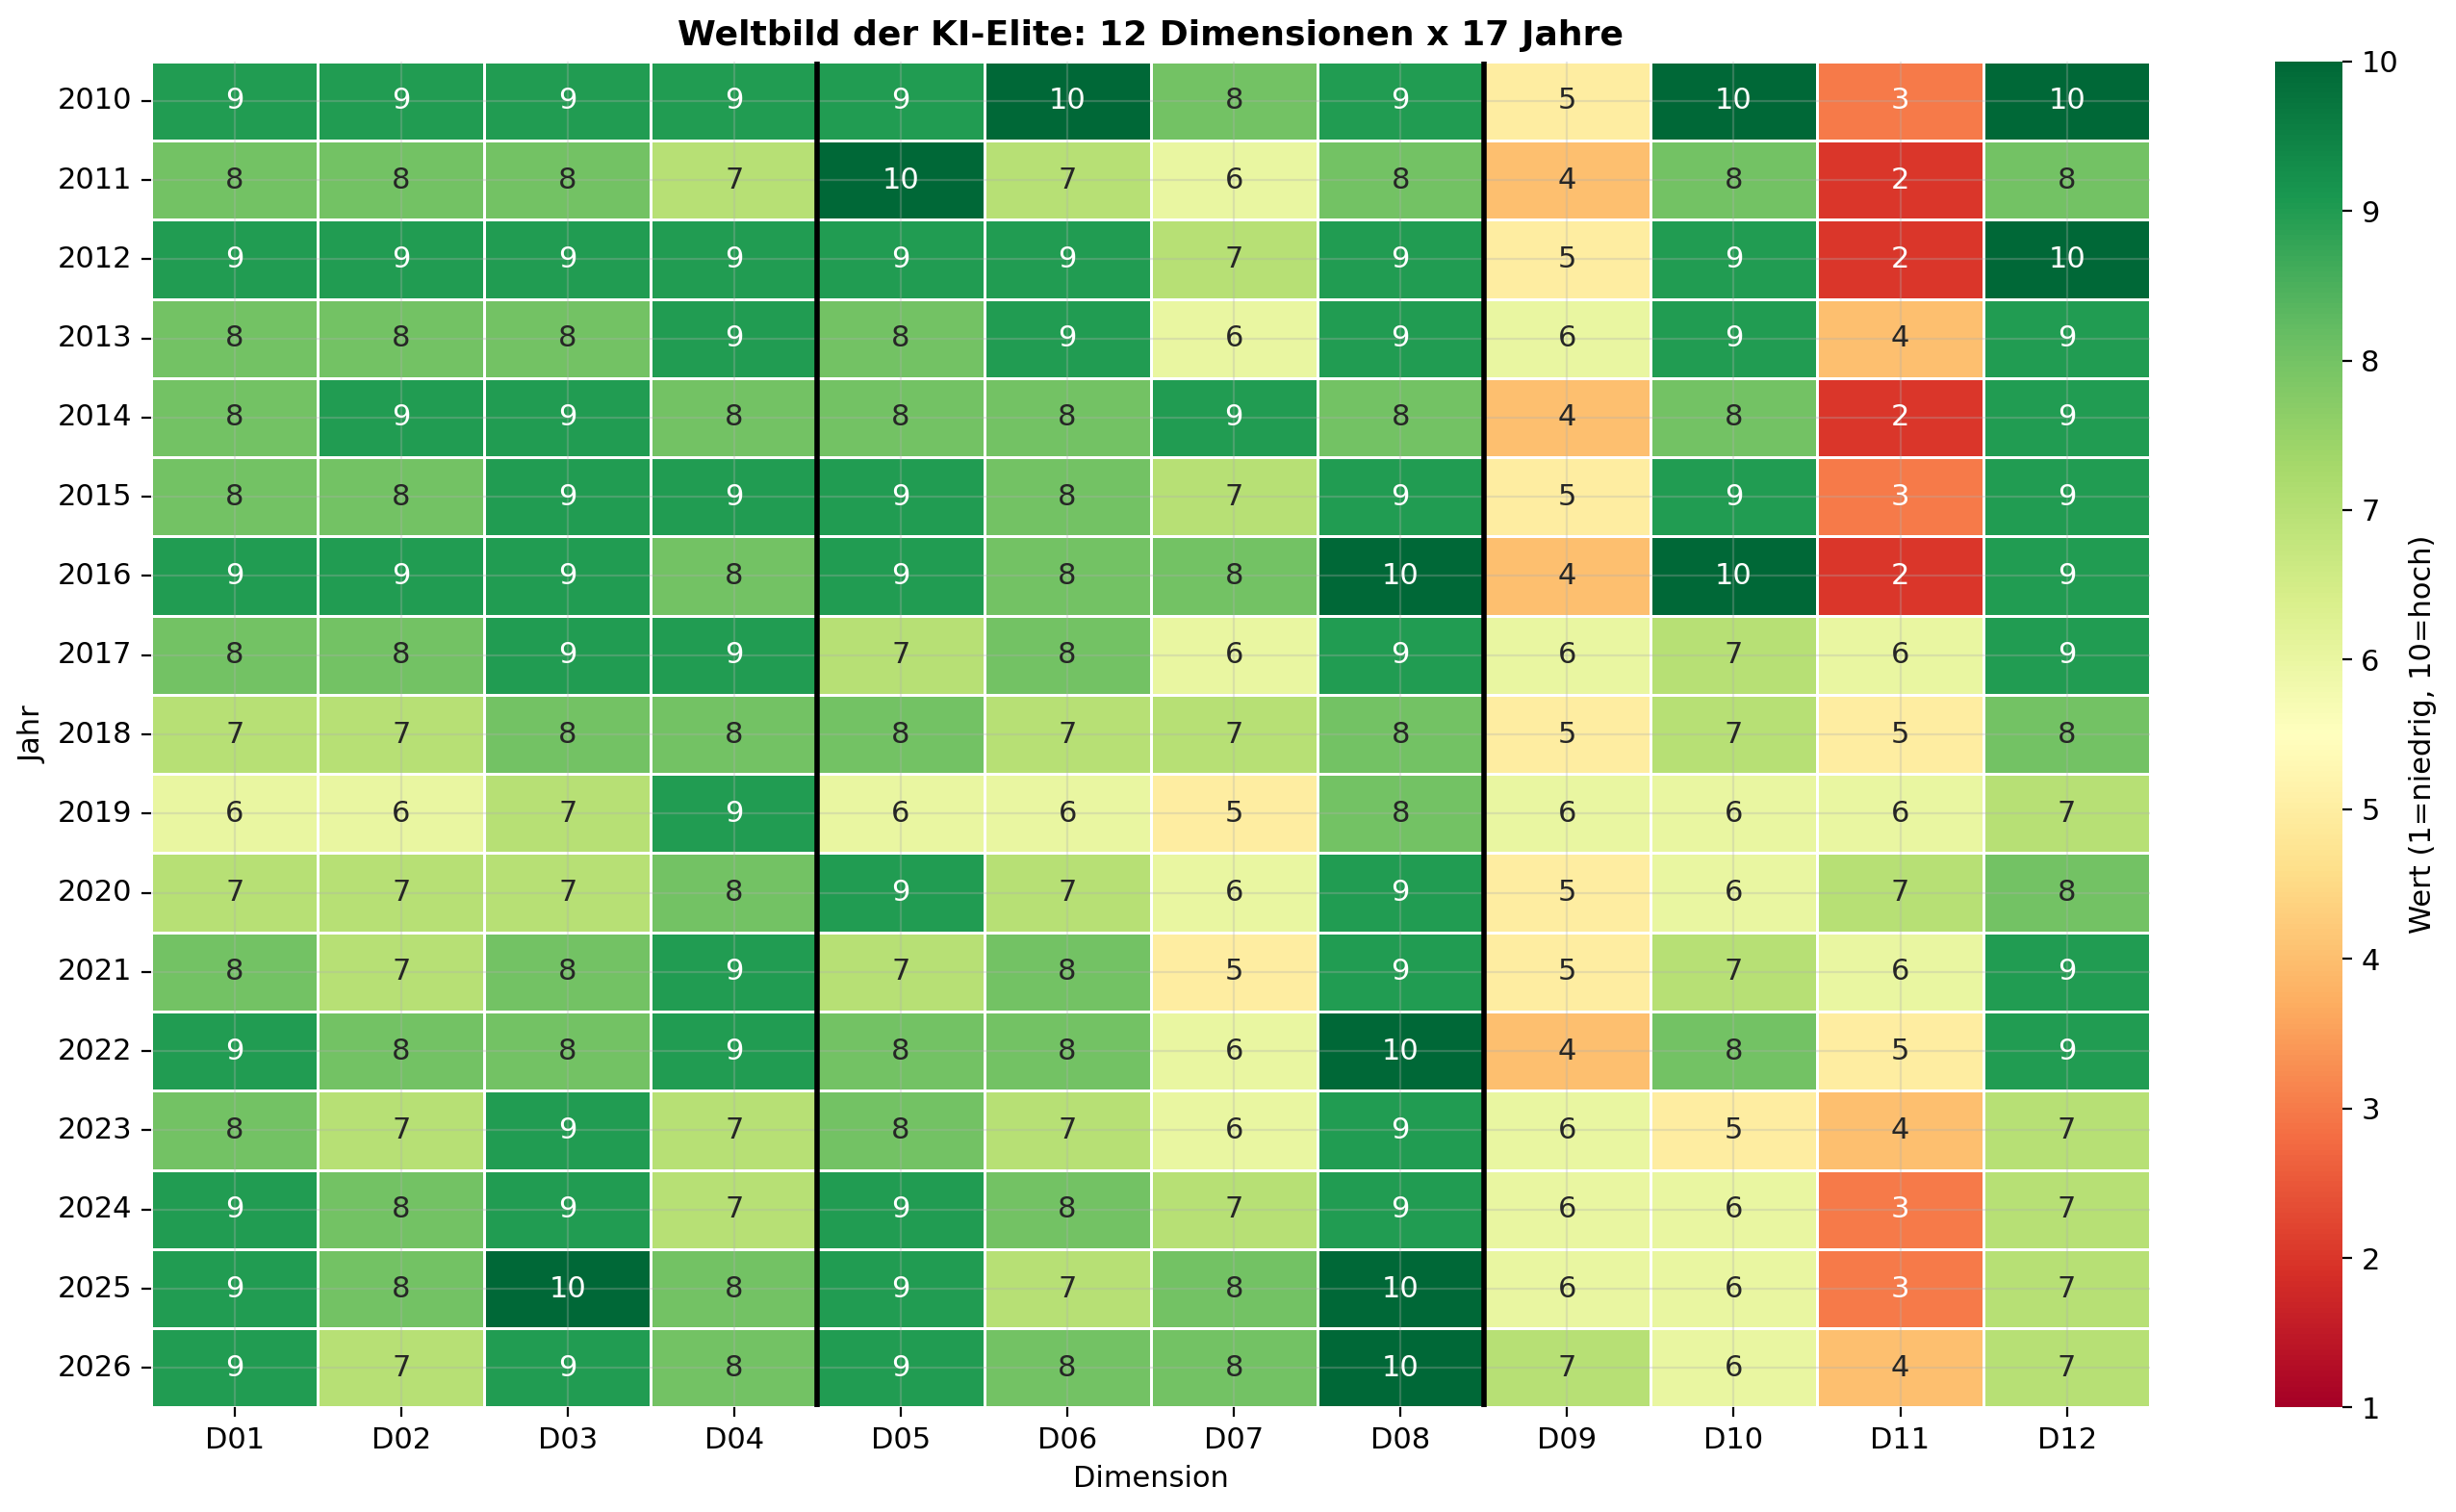
\includegraphics[width=0.95\textwidth]{fig2_heatmap.png}
  \caption{Heatmap of the 12 worldview dimensions across all analyzed groups. High values (dark) indicate intense beliefs; the dual trough at D09 and D11 is visible across all groups.}
  \label{fig:heatmap}
\end{figure}


\subsubsection{The Worldview of the Top~10}

The ten most powerful AI actors hold the same worldview in intensified form (Avg~7.7). On ten of twelve dimensions, Top~10 values lie exactly one scale point above the collective. The two exceptions: human appreciation (D09=4) and egalitarianism (D11=4) are \emph{lower}. The more powerful the position, the more pronounced the sense of mission and the more distanced the view of humanity.


\subsubsection{Core Beliefs}

The distillation of the most frequently repeated statements (SU~5: HOM\_haeuf\_A, cf.\ Appendix~\ref{app:se}) identifies five beliefs as the minimal consensus: (1)~technology as moral imperative, (2)~elite stewardship, (3)~the liberation narrative, (4)~geopolitical Manichaeism, (5)~work as identity. Safety rhetoric belongs to the core repertoire of the discourse but functions as a discursive resource, not as an action-guiding belief.

\medskip
\noindent\textbf{Core finding RQ1:} The reconstructed profiles suggest a coherent, high-intensity belief system that can be characterized as \emph{technological messianism with ambivalence structure}. The designation ``messianism'' is to be understood as an ideal-typical condensation, not as a psychological diagnosis: it denotes the specific \emph{combination} of high sense of mission (D01), techno-determinism (D05), urgency (D08), and low anthropological valuation (D09) -- a profile that goes beyond mere sense of mission because it frames technological progress as a quasi-redemptive necessity.


\subsection{RQ2 -- Change of the Worldview (Longitudinal)}
\label{sec:ergebnisse:f2}

\subsubsection{Development of the 12 Dimensions over Time}

Of twelve dimensions, four show pronounced linear trends (Table~\ref{tab:trends}).\footnote{The trend lines reported here describe \textit{patterns in reconstructed data}: the worldview values are LLM-assisted reconstructions, not independent measurements. OLS slopes and $R^2$ serve to describe the trajectory patterns, not for inferential hypothesis testing. An external validation (expert ratings vs.\ SWR output) is still pending (cf.\ Limitations section).}

\begin{table}[htbp]
  \centering
  \caption{Pronounced linear trends (OLS description, $n=17$ annual data points).}
  \label{tab:trends}
  \begin{tabular}{l l c c}
    \toprule
    \textbf{Dimension} & \textbf{Direction} & \textbf{Slope/decade} & $R^2$ \\
    \midrule
    D10 Posthumanism          & declining & $-2.4$ & $0.63$ \\
    D12 Locus of control      & declining & $-1.5$ & $0.54$ \\
    D02 Self-efficacy          & declining & $-1.0$ & $0.31$ \\
    D09 Human appreciation     & rising    & $+0.9$ & $0.27$ \\
    \bottomrule
  \end{tabular}
\end{table}

The strongest decline is in posthumanism (D10): from 10 in 2010 to 6 in 2025. The high Pearson correlation with D12 ($r = +0.85$)\footnote{The correlations reported here and below (Pearson, computed across the 17~annual data points) are \emph{associations within the LLM reconstruction}, not between independently measured variables. They could reflect internal coherence of the model rather than empirical relationships in reality (cf.\ Section~\ref{sec:limitationen}).} points to a connected phenomenon: posthumanism and locus of control erode synchronously. The only clearly rising value concerns human appreciation (D09), where the negative correlation with D10 ($r = -0.58$) suggests a compensatory linkage. The overall mean remains nearly constant (early phase 7.5, late phase 7.3), concealing a tectonic shift beneath the surface.

\begin{figure}[htbp]
  \centering
  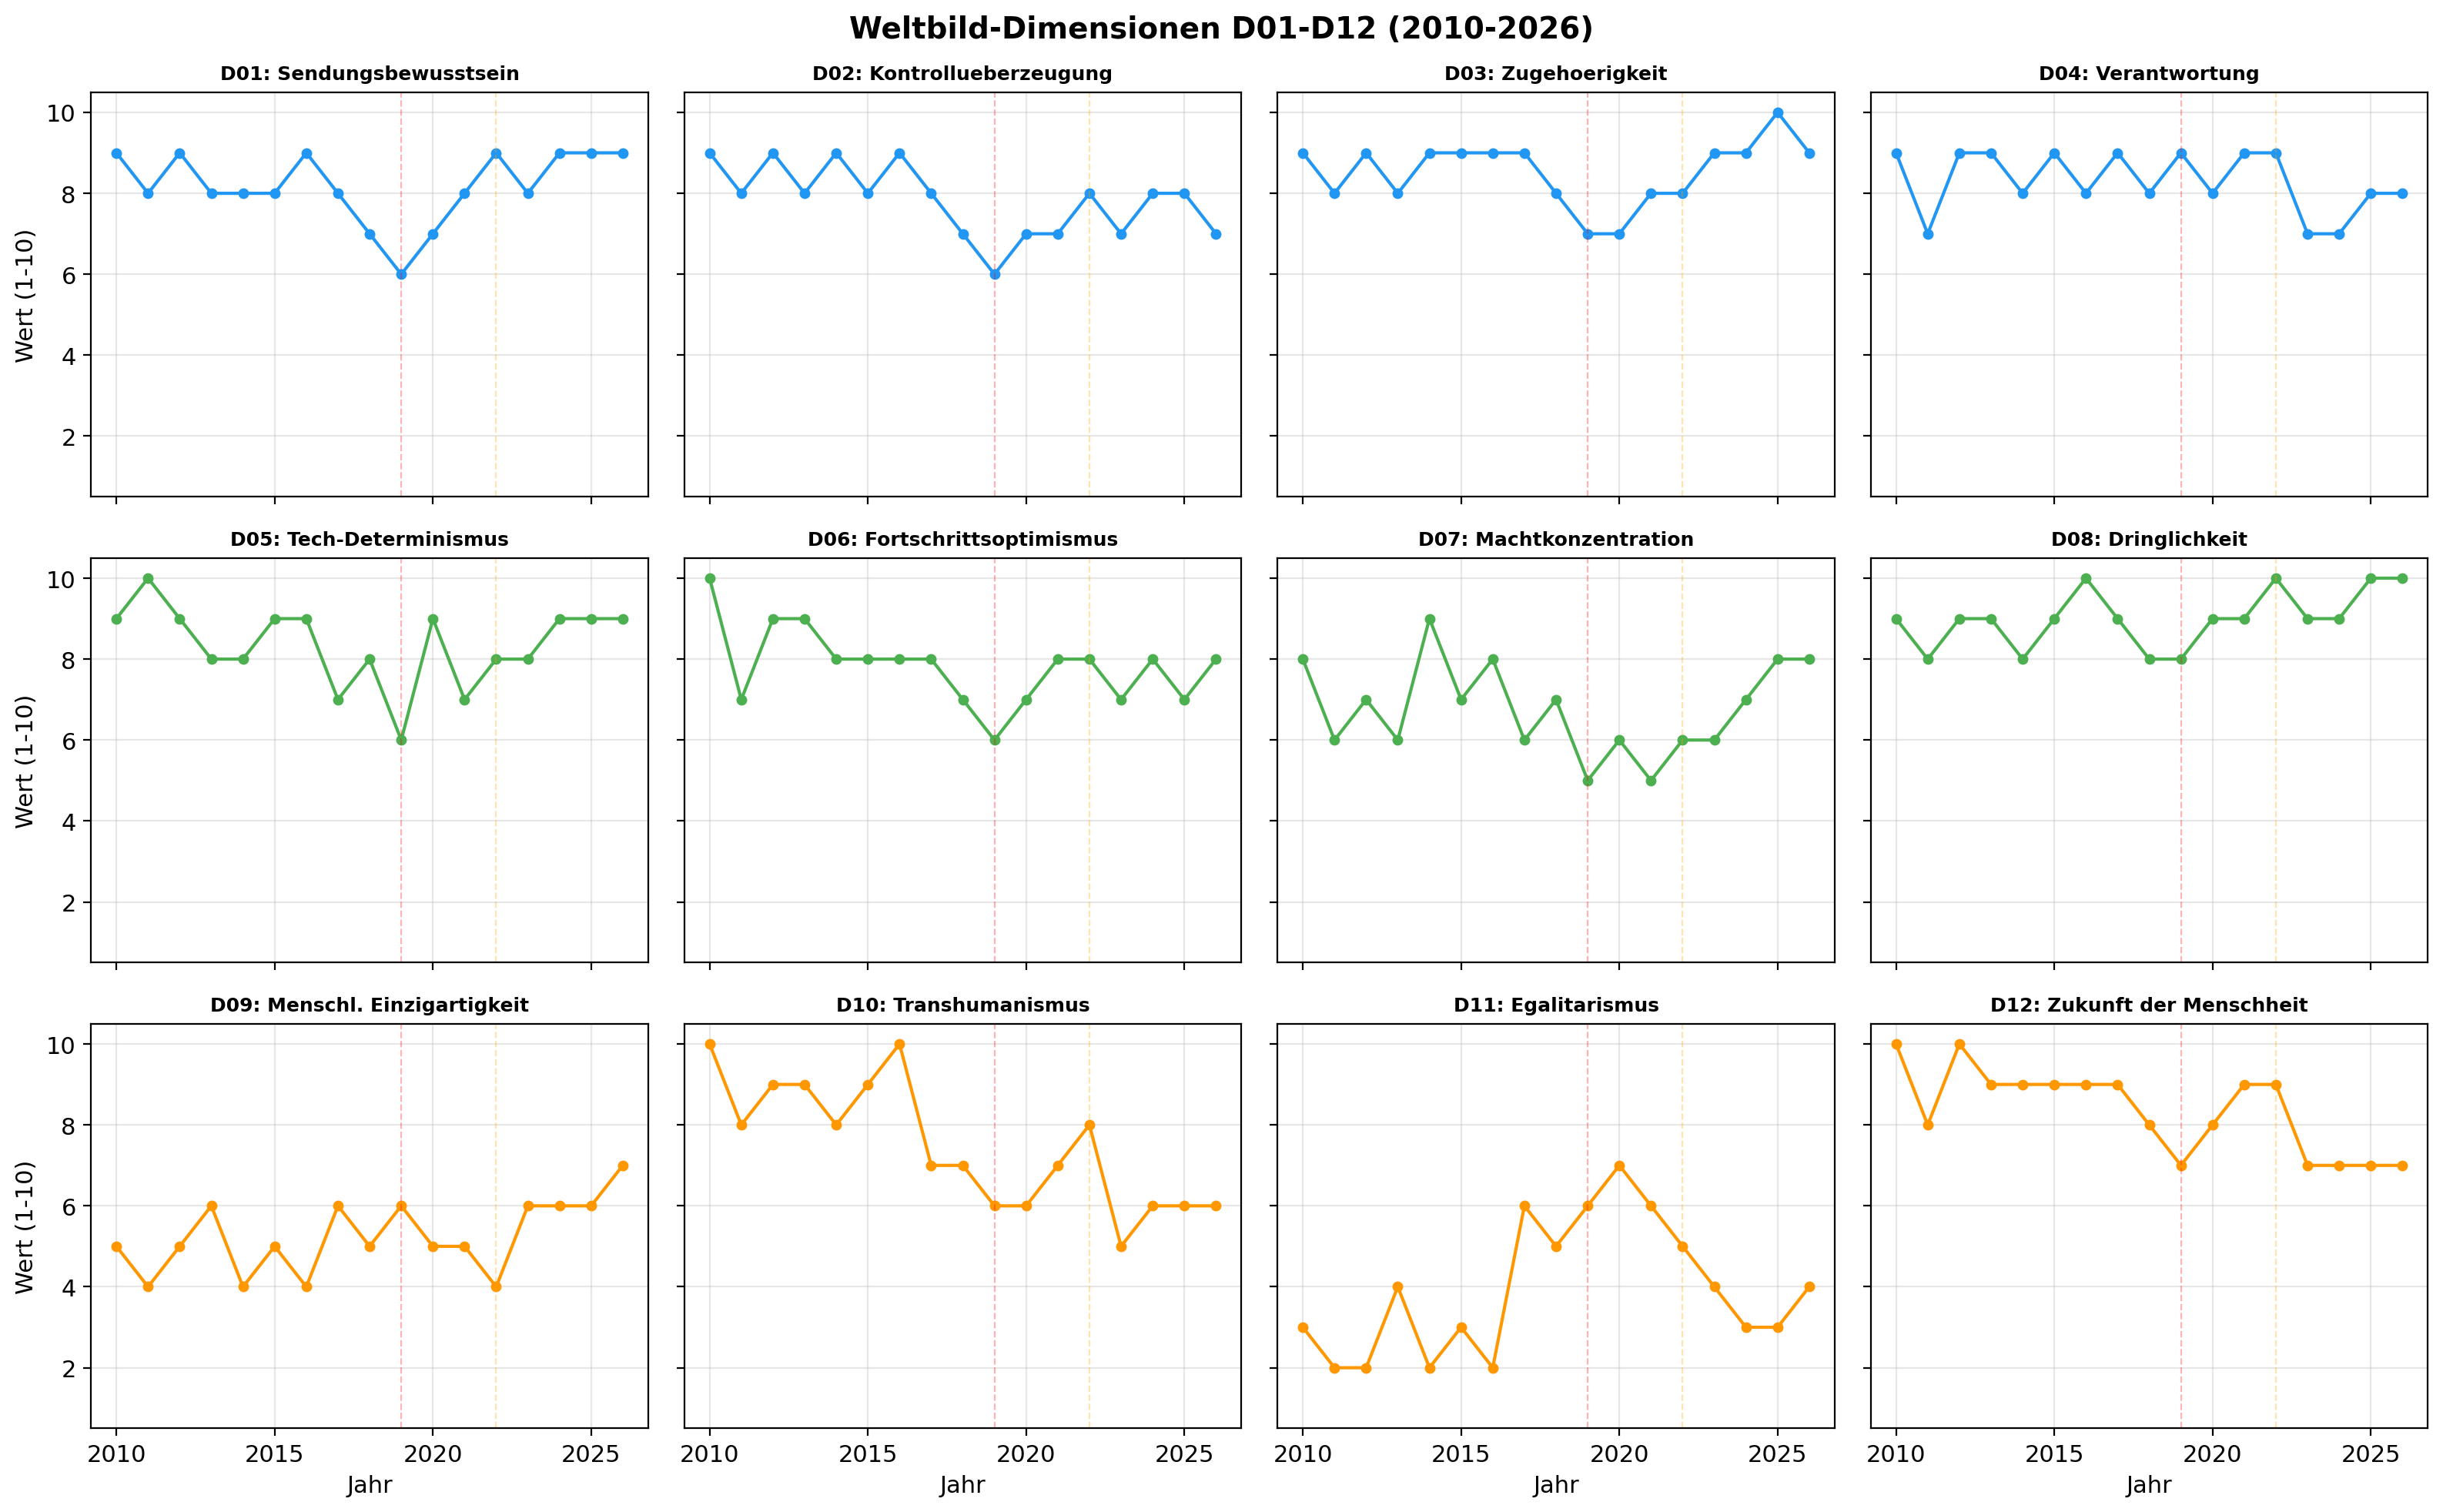
\includegraphics[width=\textwidth]{fig1_zeitreihen_panel.png}
  \caption{Time series of the 12 worldview dimensions (2010--2026). Pronounced trends are highlighted. The marked decline of D10 (posthumanism) and D12 (locus of control) constitutes the ``utopia complex,'' whose disintegration is arithmetically compensated by rising urgency (D08).}
  \label{fig:zeitreihen}
\end{figure}

\begin{figure}[htbp]
  \centering
  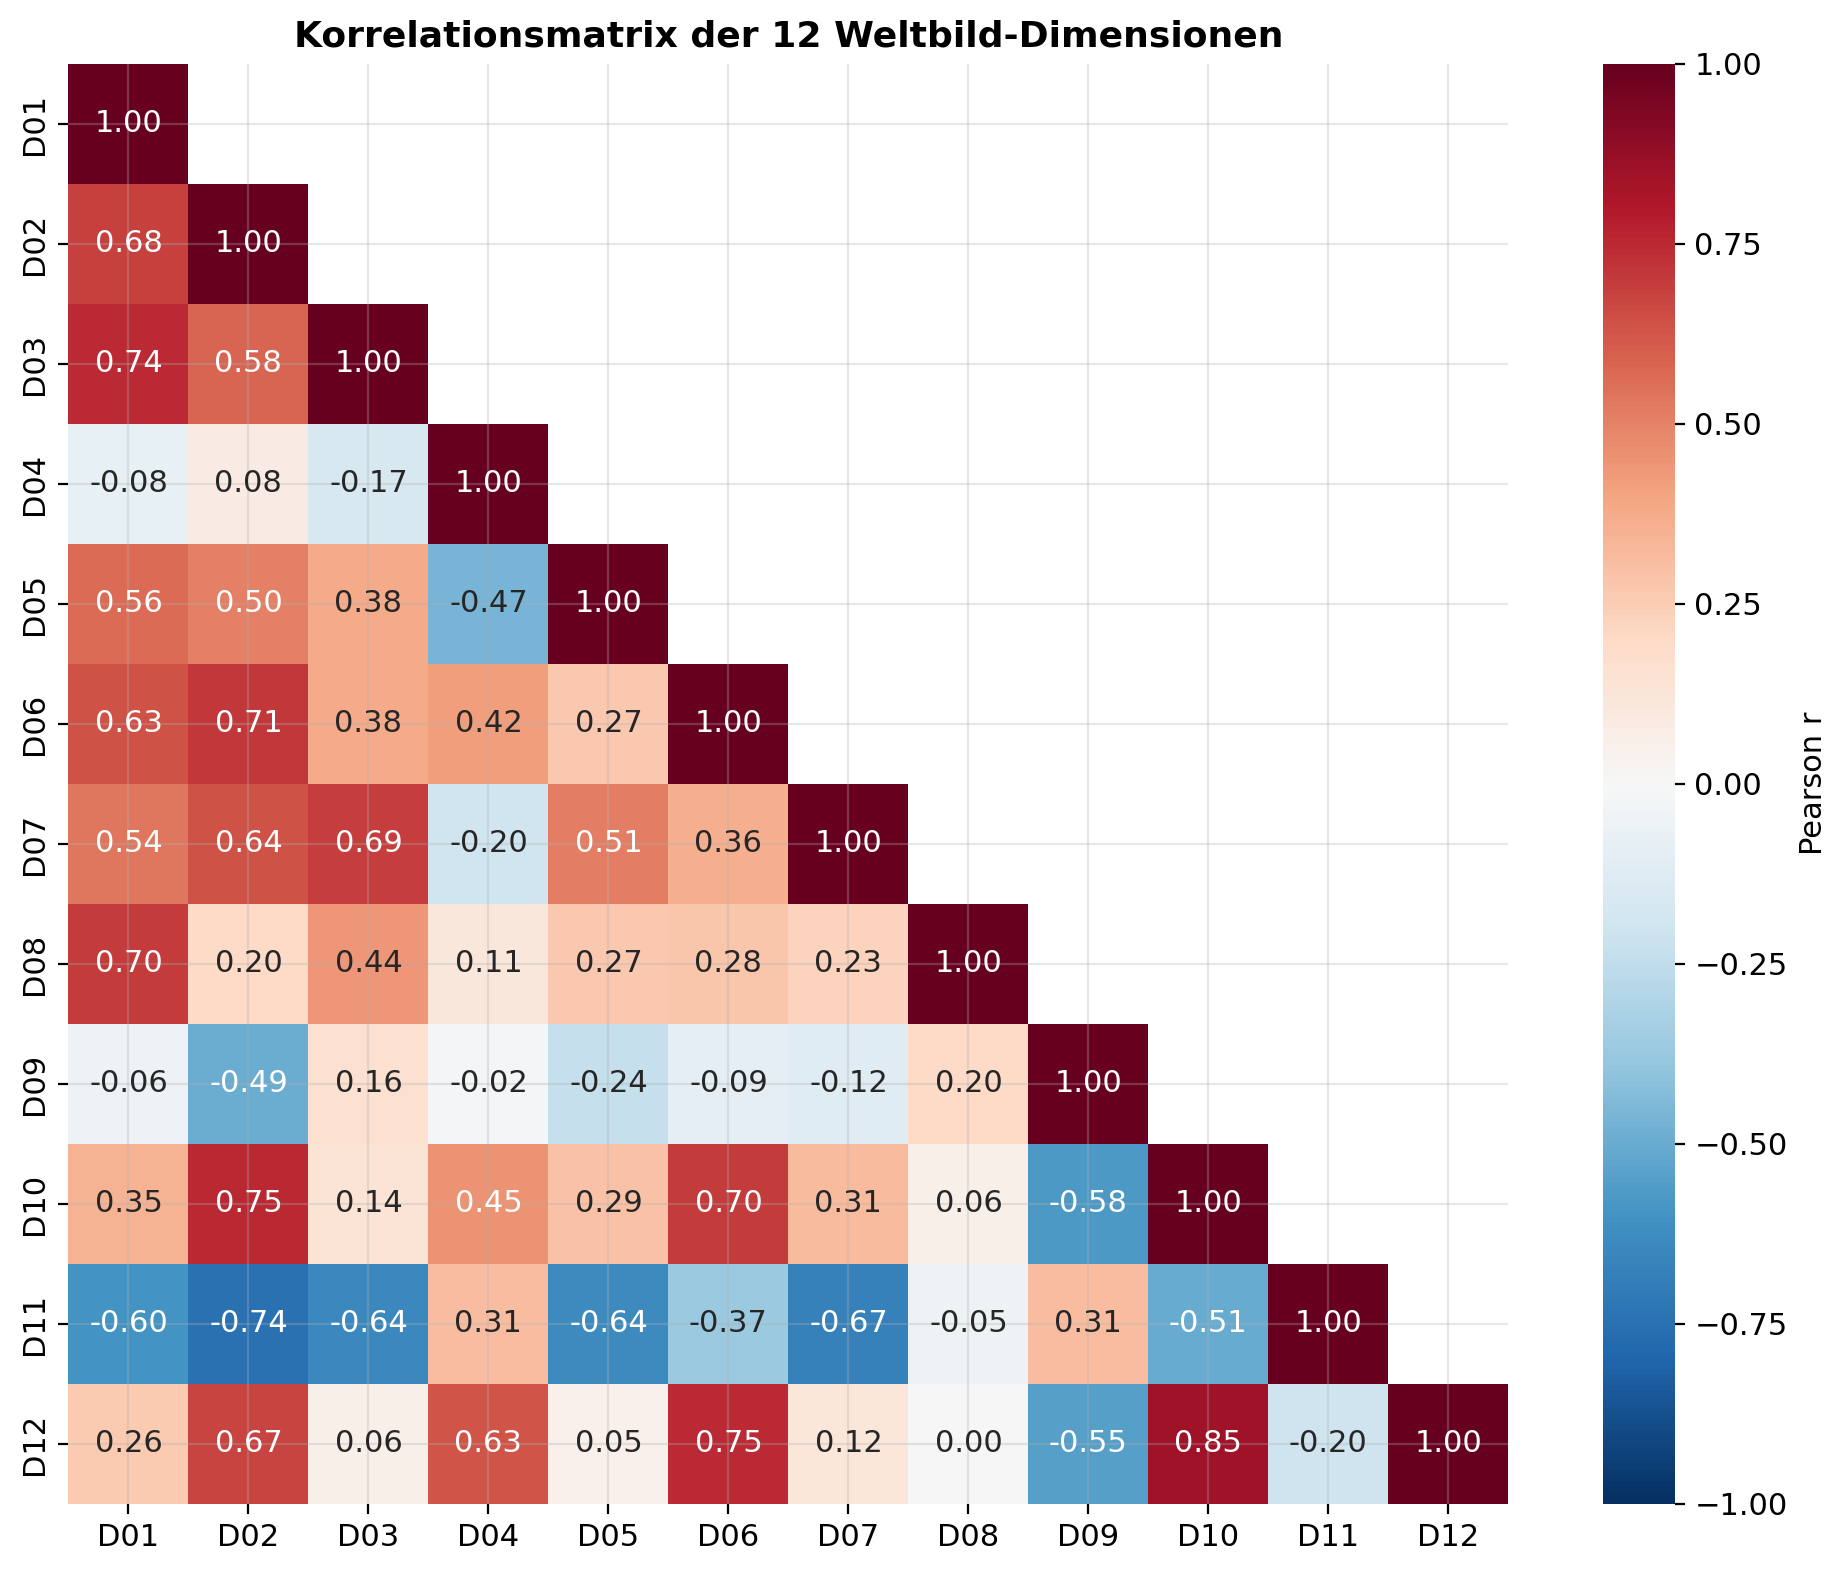
\includegraphics[width=0.85\textwidth]{fig4_korrelationsmatrix.png}
  \caption{Correlation matrix of the 12 dimensions. The strong positive correlation between D10 and D12, and the negative correlation between D10 and D09, form the empirical core of the ``utopia complex.''}
  \label{fig:korrelationsmatrix}
\end{figure}


\subsubsection{Turning Points and Epoch Comparison}

The breakpoint detection -- conducted as visual inspection of time series, supplemented by the identification of synchronous extreme points across multiple dimensions -- identifies two central turning points.\footnote{A formal breakpoint analysis (e.g., Bai-Perron test) was not meaningfully applicable due to the small number of time points ($n=17$) and the nature of the data (LLM reconstructions, not independent measurements). The turning points are therefore to be understood as \emph{descriptive observations}, not as statistically confirmed structural breaks.} The first lies at 2019: four dimensions (D01, D02, D05, D06) reach synchronous lows, temporally associated with the GPT-2 withholding decision. The second, more permanent turning point lies at 2022/2023: contemporaneous with the ChatGPT release, a marked pattern shift emerges -- urgency reaches its reconstructed maximum (D08=10), egalitarianism drops from 6 to 4. Unlike 2019, the values do not return; the reconstructed profiles after 2022 suggest a new equilibrium.

\begin{figure}[htbp]
  \centering
  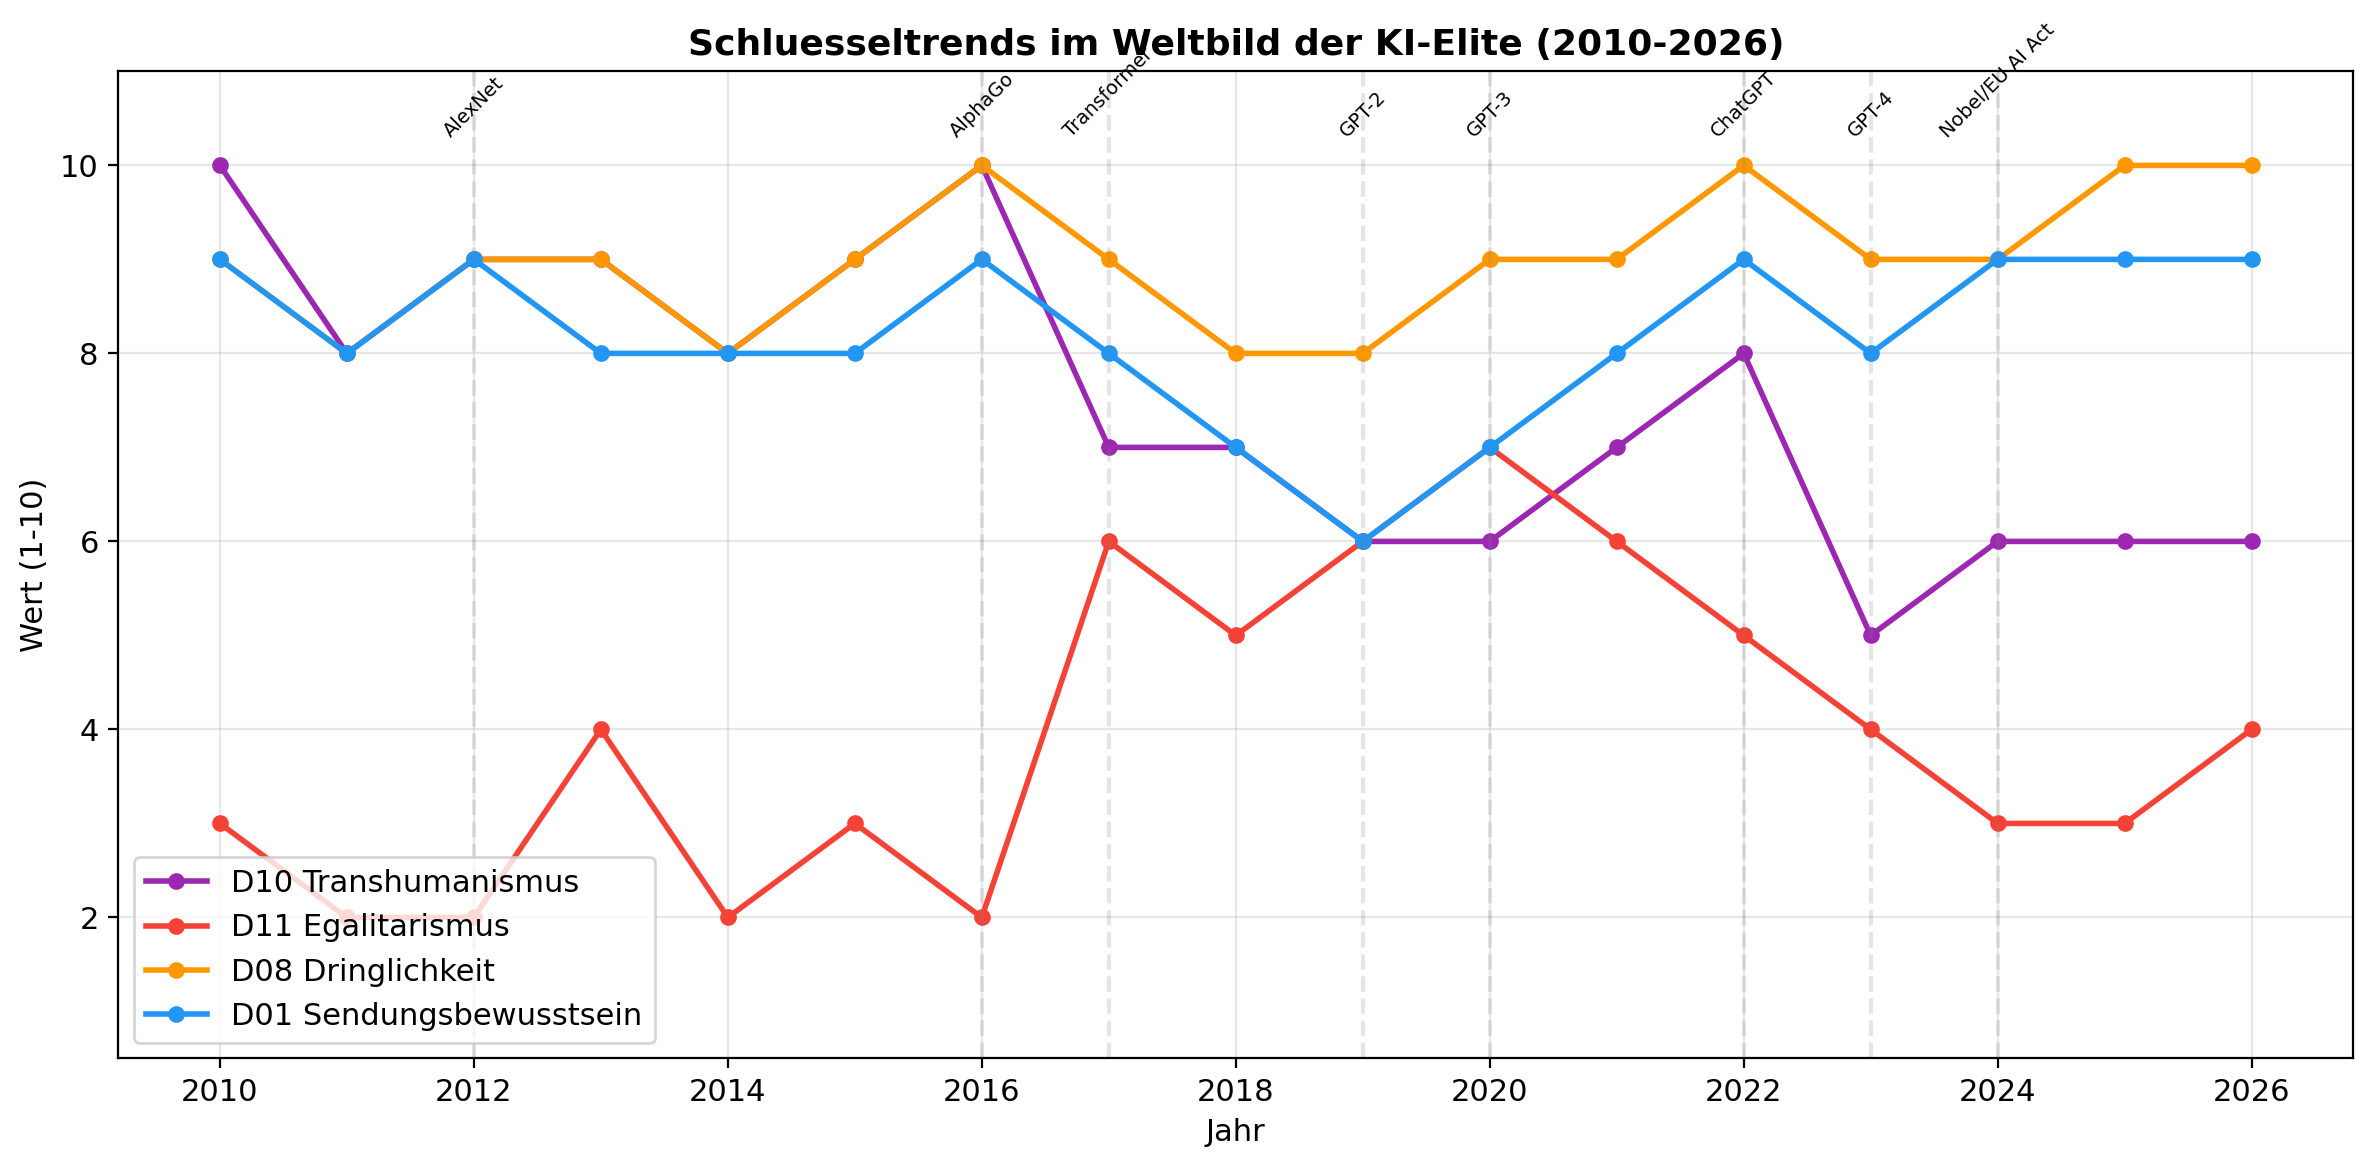
\includegraphics[width=0.95\textwidth]{fig7_schluesseltrends.png}
  \caption{Key trends of the worldview transformation. The two turning points (2019, 2022/2023) and three epochs (Promethean Optimism, First Ambivalence, Tragic Consciousness) are marked.}
  \label{fig:schluesseltrends}
\end{figure}


\subsubsection{Convergence or Divergence?}

The data show increasing differentiation. The ChatGPT effect intensifies both the Architect position (acceleration, power concentration) and the Guardian position (caution, regulation) simultaneously -- it acts as a catalyst for bipolarization.


\subsubsection{Metaphor and Emotion Shift}

The guiding metaphor shifts from Prometheus -- the fire-bringer -- to the tragic hero who must save what may no longer be savable. The action remains the same (acceleration), but its emotional framing reverses: no longer from euphoria, but from the belief that the alternative would be worse.

\medskip
\noindent\textbf{Core finding RQ2:} The worldview has structurally transformed -- from a monochrome utopia to a bimodal wager. Three erosion trends (D10, D12, D02) form a ``utopia complex'' whose disintegration is arithmetically compensated by rising urgency.


\subsection{RQ3 -- Congruence of Statements and Actions}
\label{sec:ergebnisse:f3}

\begin{table}[htbp]
  \centering
  \caption{Comparison of statements (S) and actions (A), $N=100$.}
  \label{tab:kongruenz}
  \begin{tabular}{l c c c l}
    \toprule
    \textbf{Dimension} & \textbf{Say} & \textbf{Do} & $\Delta$ & \textbf{Assessment} \\
    \midrule
    D01 Sense of mission        & 8 & 7 & $-1$ & Slight \\
    D02 Self-efficacy           & 8 & 9 & $+1$ & Do $>$ Say \\
    D03 Work ethic              & 8 & 9 & $+1$ & Do $>$ Say \\
    D04 Sense of responsibility & 7 & 5 & $\mathbf{-2}$ & Strong \\
    D05 Techno-determinism      & 8 & 9 & $+1$ & Do $>$ Say \\
    D06 Belief in progress      & 8 & 6 & $\mathbf{-2}$ & Strong \\
    D07 Power concentration     & 6 & 8 & $\mathbf{+2}$ & Strong \\
    D08 Urgency                 & 8 & 9 & $+1$ & Do $>$ Say \\
    D09 Human appreciation      & 5 & 3 & $\mathbf{-2}$ & Strong \\
    D10 Posthumanism            & 7 & 8 & $+1$ & Do $>$ Say \\
    D11 Egalitarianism          & 5 & 2 & $\mathbf{-3}$ & \textbf{Massive} \\
    D12 Locus of control        & 8 & 7 & $-1$ & Slight \\
    \midrule
    \textbf{Mean}               & \textbf{7.2} & \textbf{6.8} & $-0.4$ & \\
    \bottomrule
  \end{tabular}
\end{table}

The discrepancies arrange themselves into two complementary clusters. The \emph{downward cluster} (Do $<$ Say) encompasses the society-oriented dimensions: egalitarianism ($\Delta\,-3$), sense of responsibility, belief in progress, and human appreciation (each $\Delta\,-2$). The \emph{upward cluster} (Do $>$ Say) encompasses the power-related dimensions: power concentration ($\Delta\,+2$), self-efficacy, work ethic, techno-determinism (each $\Delta\,+1$). The resulting pattern: a systematic self-presentation asymmetry. Publicly, the AI elite presents itself as more moderate, more responsible, and more egalitarian than it acts in practice.

\begin{figure}[htbp]
  \centering
  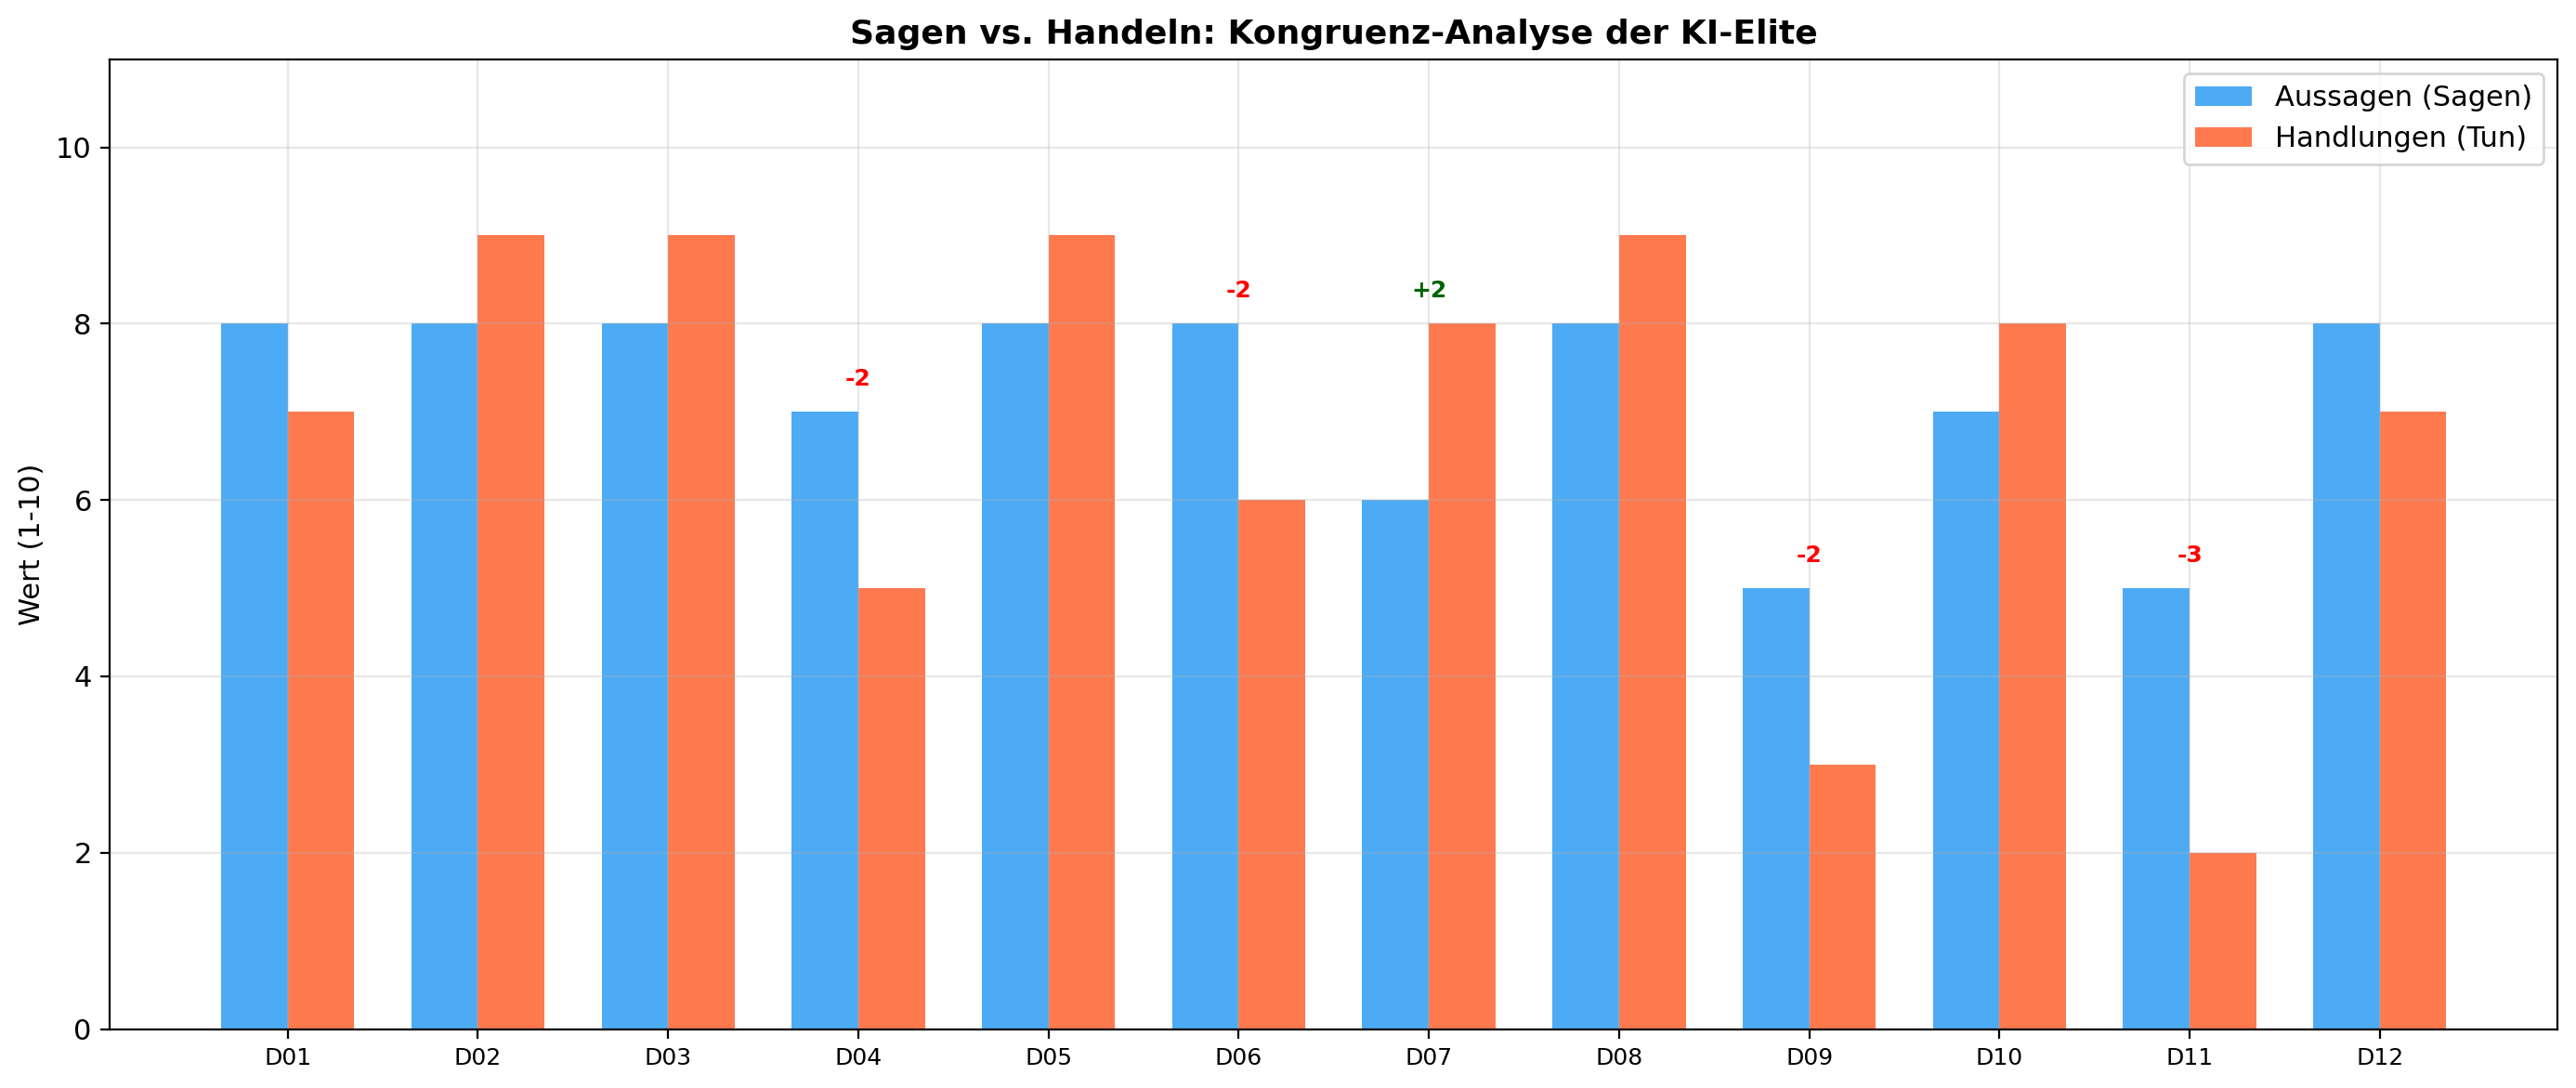
\includegraphics[width=0.95\textwidth]{fig6_sagen_vs_handeln.png}
  \caption{Say vs.\ Do: comparison of worldviews reconstructed from statements (S) and actions (A). The society-oriented dimensions (D04, D06, D09, D11) systematically decline in action, while power-related dimensions (D07, D05) rise.}
  \label{fig:sagen_handeln}
\end{figure}

The most massive single discrepancy ($\Delta\,-3$ at D11) shows: in statements, the AI elite speaks of ``access for all''; in their actions, they build dual-class share structures, concentrate compute infrastructure, and create exclusive networks. For context: a $\Delta$ of 3 on a 10-point scale corresponds to nearly one-third of the entire scale range -- a difference that, in substantive interpretation, must be considered substantial.\footnote{A formal effect size calculation (e.g., Cohen's $d$) is not possible here, since no individual-level dispersion measures are available. The classification as ``large'' is based on substantive interpretation of the scale range, not on psychometric conventions.}

\medskip
\noindent\textbf{Core finding RQ3:} The incongruence is systematic, directional, and functional. The data suggest that the AI elite means what it says about its own significance -- but not what it says about equality, responsibility, and humanity.


\subsection{RQ4 -- Worldview Clusters}
\label{sec:ergebnisse:f4}

Four distinct worldview types can be identified from the data (Table~\ref{tab:typen}).

\textbf{Identification method:} Cluster identification followed a two-stage procedure. \emph{Stage~1 (LLM-assisted):} All 15 group syntheses were grouped by similarity patterns across the 12~dimensions, with the largest variance axes (D07~power concentration, D09~human appreciation, D11~egalitarianism) serving as discriminating features. \emph{Stage~2 (author validation):} The four-cluster solution proposed by the LLM was evaluated by the author for substantive coherence and plausibility. Alternative solutions (three and five clusters) were examined and rejected: three clusters merge Innovator and Liberator, which is not substantively justified; five clusters split the Guardian type into a subgroup that could not be stably reproduced. We emphasize that this cluster identification is \emph{exploratory} -- a confirmatory validation on an independent dataset is pending. The cluster solution is an \emph{interpretive hypothesis}, not a statistically confirmed result in the sense of formal cluster analysis.

\begin{table}[htbp]
  \centering
  \caption{The four worldview types of the AI elite.}
  \label{tab:typen}
  \small
  \begin{tabular}{l c c c c}
    \toprule
    \textbf{Feature} & \textbf{I ``Architect''} & \textbf{II ``Guardian''} & \textbf{III ``Innovator''} & \textbf{IV ``Liberator''} \\
    \midrule
    $n$ & 35 & 25 & 22 & 18 \\
    Prototype & CEOs, investors & Academics, risk warn. & Founders & Open source \\
    Avg D01--D12 & 7.8 & 6.4 & 7.2 & 6.8 \\
    D04 Responsibility & 6.3 & \textbf{9.0} & 8.3 & 6.0 \\
    D07 Power conc. & \textbf{8.8} & 4.8 & 6.5 & \textbf{2.5} \\
    D09 Human appr. & \textbf{3.3} & 5.8 & 4.8 & \textbf{6.5} \\
    D11 Egalitarianism & \textbf{2.8} & \textbf{7.2} & 5.0 & \textbf{7.5} \\
    \bottomrule
  \end{tabular}
\end{table}

The \textbf{Architect} combines maximal sense of mission with minimal egalitarianism: power concentration is the prerequisite for agency. The \textbf{Guardian} forms the counterpoint: maximal responsibility, demand for institutional constraint. The \textbf{Innovator} occupies a middle position. The \textbf{Liberator} is the most surprising discovery: minimal power concentration \emph{and} high egalitarianism -- anti-regulation actors who want to distribute power more radically than anyone else, albeit through markets and open-source communities.\footnote{The high D11 value of the Liberator type (7.5) and the low D11 value of individual prototypes (e.g., Andreessen: D11=2) mark a construct validity tension: D11 measures orientation toward equality, not its \emph{mechanism}. Market-libertarian access egalitarianism (Liberator) and redistributive egalitarianism (Guardian) produce similar scale values on D11 but mean different things. The prototype value refers to the individual-person synthesis, the cluster value to the group aggregate -- Andreessen's individual profile deviates from the cluster mean. Future operationalizations should differentiate here.}

\begin{figure}[htbp]
  \centering
  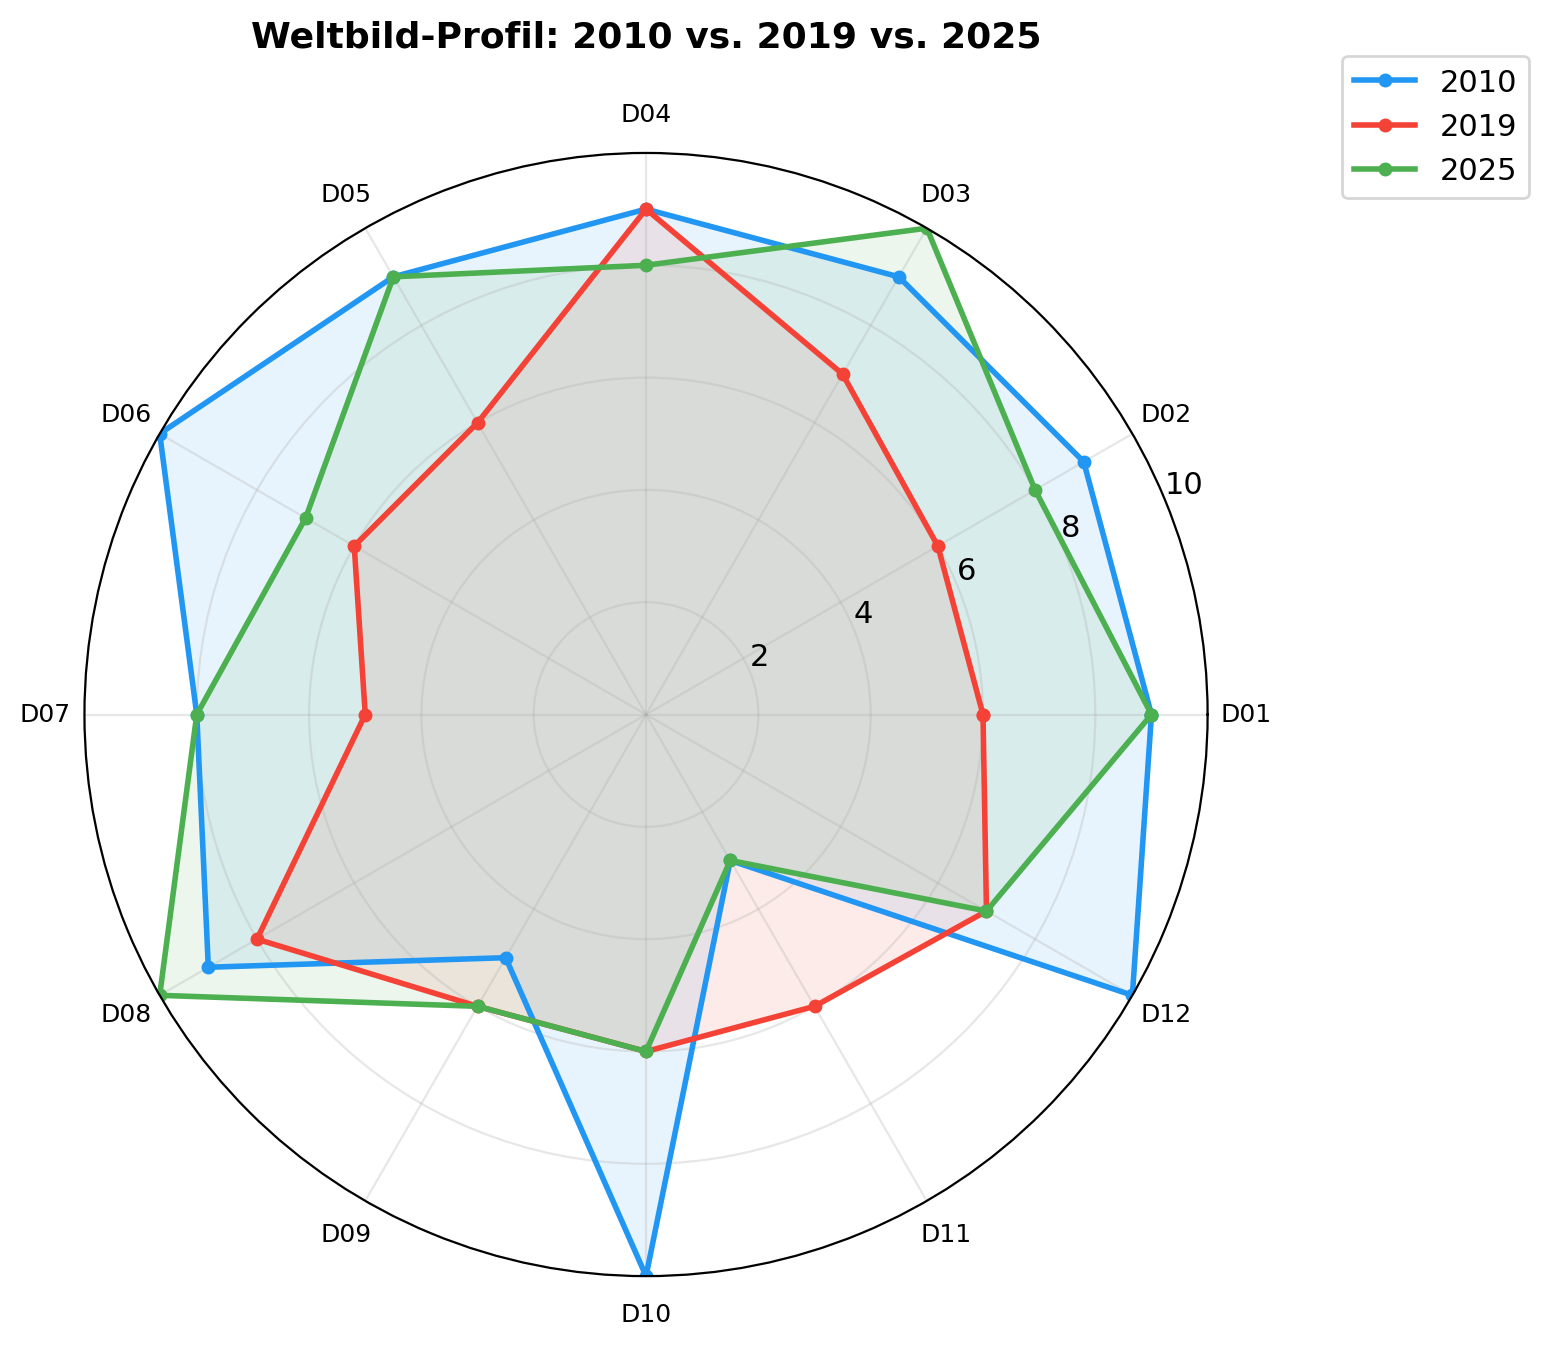
\includegraphics[width=0.85\textwidth]{fig3_radar_vergleich.png}
  \caption{Radar chart of the four worldview types across the 12 dimensions. The polarization between Architect (outer) and Guardian (inner), and the surprising position of the Liberator, are clearly visible.}
  \label{fig:radar}
\end{figure}

\medskip
\noindent\textbf{Core finding RQ4:} The strongest polarization exists between Type~I (logic of domination) and Type~II (logic of participation). The power-moderation paradox -- resource control correlates inversely with egalitarianism and responsibility -- is the finding most critical for democratic theory.


\subsection{RQ5 -- Subgroup Comparisons}
\label{sec:ergebnisse:f5}

\begin{table}[htbp]
  \centering
  \caption{Ranking of subgroup differences.}
  \label{tab:subgruppen}
  \small
  \begin{tabular}{c l c c c l}
    \toprule
    \textbf{Rank} & \textbf{Comparison} & \textbf{Avg A} & \textbf{Avg B} & $\Delta$ & \textbf{Strongest contrast} \\
    \midrule
    1 & Risk vs.\ Speed     & 5.9 & 7.6 & 1.7 & D02, D06, D10, D12: each $-5$ \\
    2 & CEOs vs.\ Academics  & 7.8 & 6.3 & 1.5 & D07: $+4$, D11: $-4$ \\
    3 & Women vs.\ Men       & 6.9 & 8.1 & 1.2 & D11: $-6$ \\
    4 & Open vs.\ Closed     & 6.8 & 6.3 & 0.5 & D07: $-3$, D12: $+3$ \\
    5 & Reg-pro vs.\ Contra  & 6.3 & 6.8 & 0.5 & D04: $+4$, D06: $-3$ \\
    6 & Anthropic vs.\ OpenAI & 6.9 & 7.3 & 0.4 & D12: $-3$ \\
    \bottomrule
  \end{tabular}
\end{table}

\begin{figure}[htbp]
  \centering
  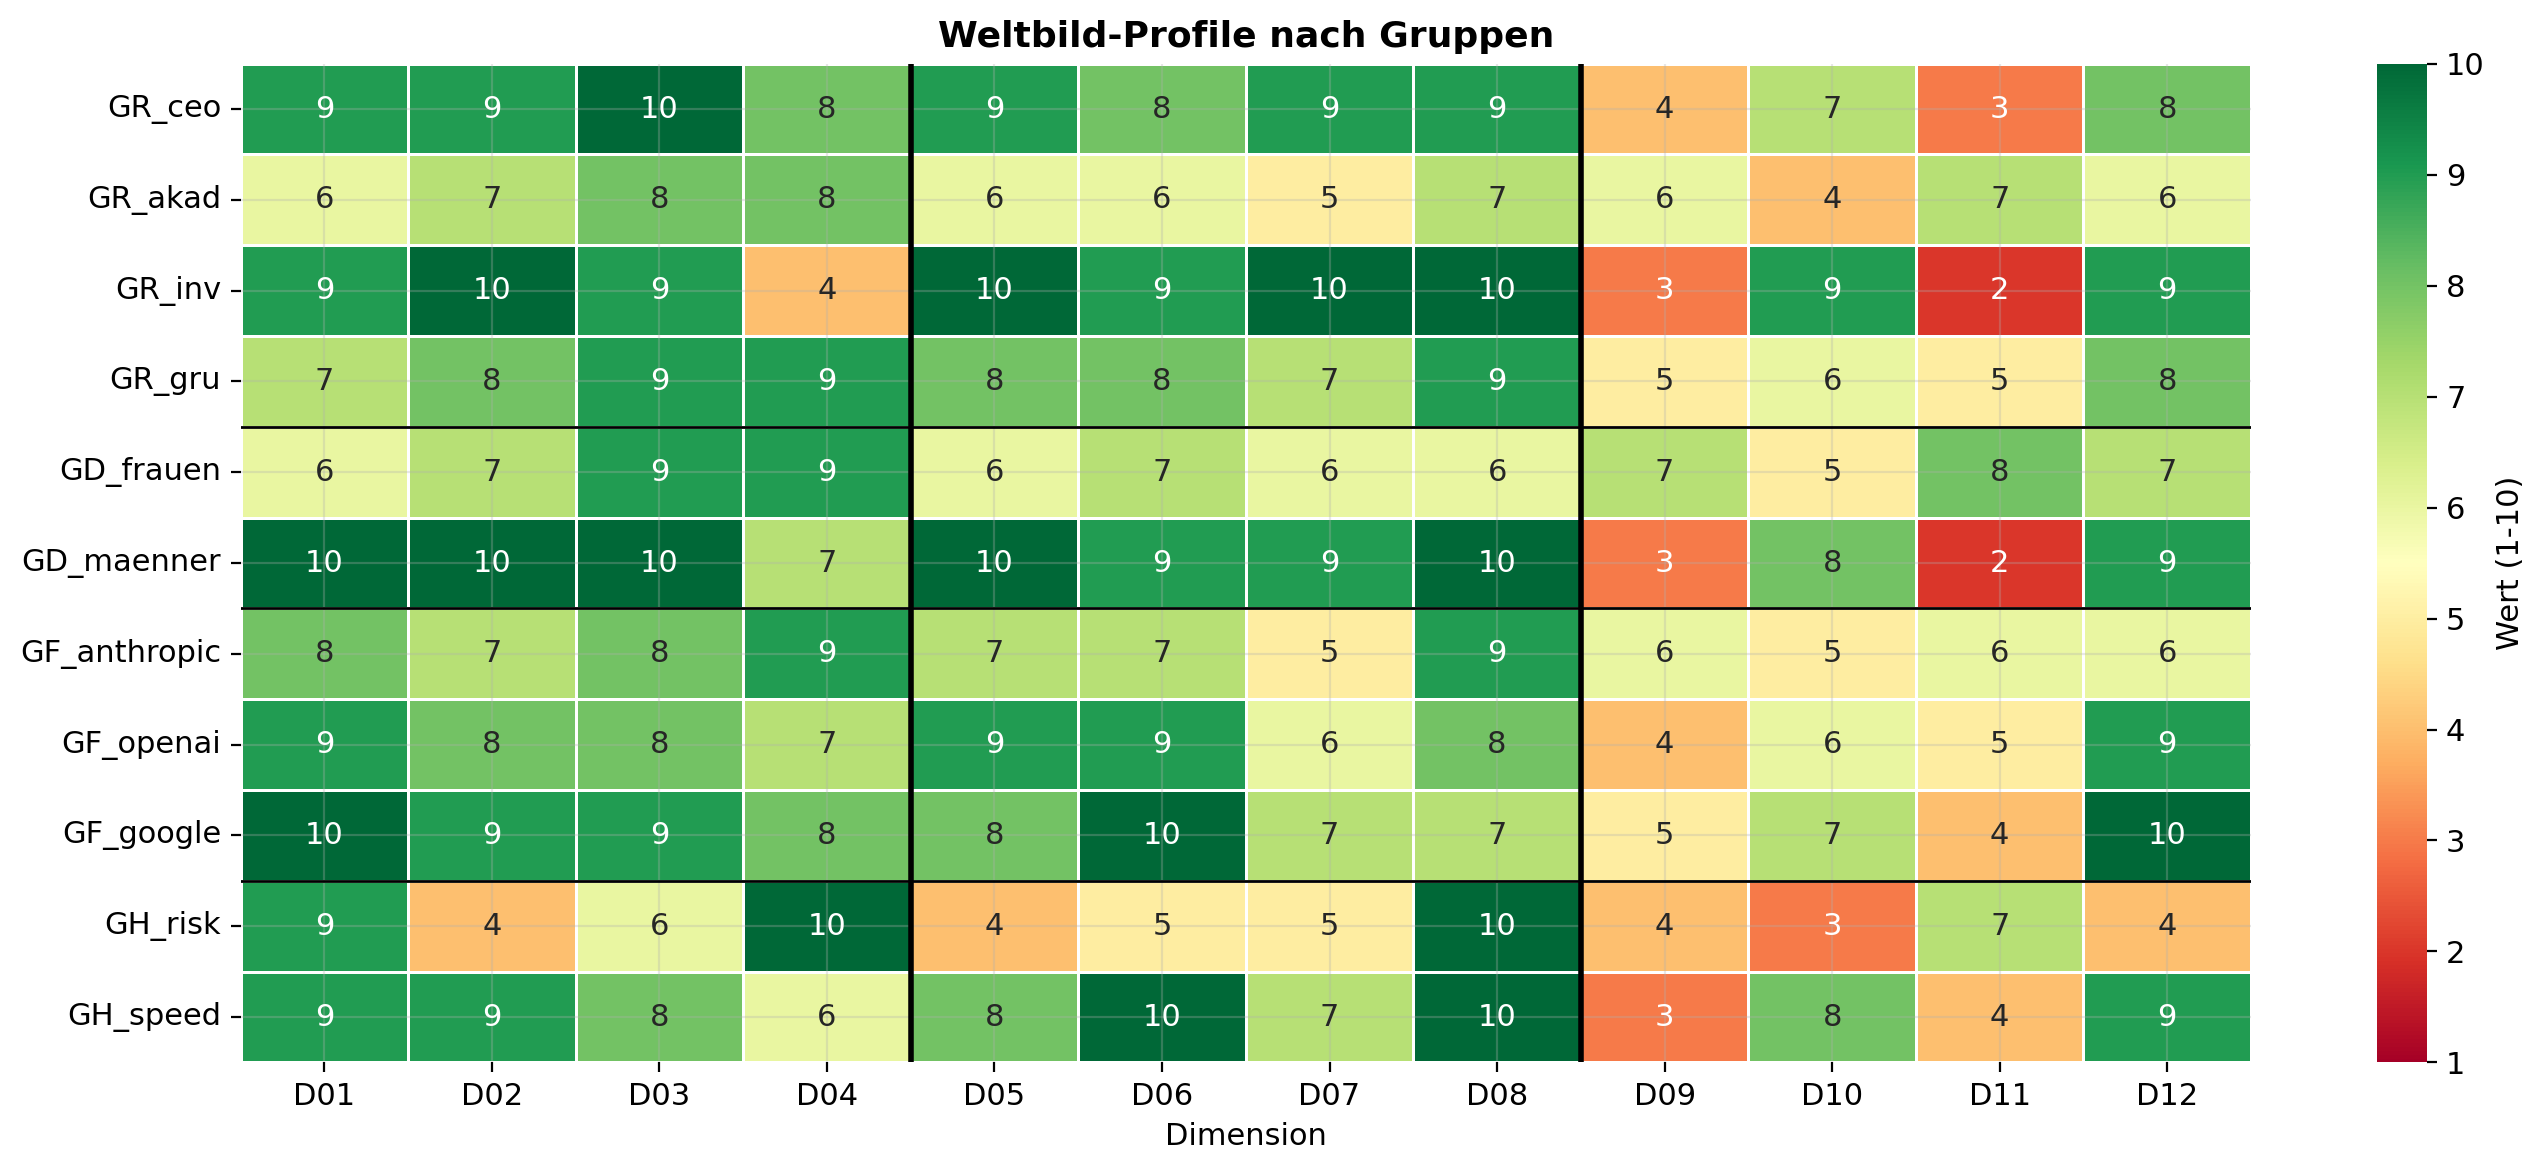
\includegraphics[width=\textwidth]{fig5_gruppen_heatmap.png}
  \caption{Group heatmap: 15 subgroups $\times$ 12 dimensions. The systematic variation of D07 (power concentration) and D11 (egalitarianism) across all comparisons is the central visual finding.}
  \label{fig:gruppen_heatmap}
\end{figure}

The \textbf{strongest contrast} (Risk vs.\ Speed, $\Delta$~1.7) does not concern risk assessment -- both sides estimate catastrophe probability at 10--20\% -- but the ontological pre-commitment: risk warners conceive of AI as a potential autonomous agent, accelerators as a tool.

The \textbf{largest nominal single contrast} in the entire survey is found at D11 in the gender comparison: six full scale points (Women:~8, Men:~2). The female worldview is not an anti-technology worldview but a \emph{conditioned} technology worldview: equally optimistic but with stronger ethical conditions. This finding, however, is the \emph{most contamination-prone} of the entire study and is therefore classified as a \emph{preliminary hypothesis}, not as a confirmed finding. The reasons: (a)~LLMs reproduce known gender stereotypes, especially the attribution of heightened social orientation to women \citep{Santurkar2023}; (b)~the female subsample is small ($n = 18$); (c)~the effect size ($\Delta = 6$) markedly exceeds what comparable empirical studies have observed. An independent validation -- ideally through multi-LLM triangulation and expert ratings -- is particularly urgent for this finding.

The \textbf{biggest surprise} lies in the regulation comparison: anti-regulators have the lowest power concentration value of all 15~groups (D07=2). This contradicts the widespread narrative that anti-regulators represent corporate interests.

\medskip
\noindent\textbf{Core finding RQ5:} The three strongest predictors of worldview are ideological stance, institutional role, and gender. The most polarizing dimensions are D11 and D07. The \emph{question of power} is the core of internal differences.


\subsection{RQ6 -- Power and Worldview}
\label{sec:ergebnisse:f6}

\emph{Power} is understood operationally in this study as resource control: the ability to command capital, compute infrastructure, research teams, and political access, and thereby influence the direction of AI development. This definition follows the sociological concept of power in the sense of Weber (``the chance to impose one's own will even against resistance'') and Bourdieu (capital accumulation as a power mechanism), without claiming a comprehensive power-theoretical analysis.

\begin{table}[htbp]
  \centering
  \caption{Worldview types and resource control.}
  \label{tab:macht}
  \begin{tabular}{l c c c l}
    \toprule
    \textbf{Type} & \textbf{Avg} & \textbf{D11} & \textbf{D04} & \textbf{Resources} \\
    \midrule
    I Architect   & 7.8 & 2.8 & 6.3 & Highest \\
    III Innovator & 7.2 & 5.0 & 8.3 & High \\
    IV Liberator  & 6.8 & 7.5 & 6.0 & Medium \\
    II Guardian   & 6.4 & 7.2 & 9.0 & Lowest \\
    \bottomrule
  \end{tabular}
\end{table}

The higher the worldview intensity, the lower the values for human appreciation and egalitarianism, and the higher the acceptance of power concentration. The investor profile marks the extreme case: maximal locus of control (D02=10) with minimal sense of responsibility (D04=4) -- ``power without accountability.'' The Top~10 lie exactly one point above the collective on ten of twelve dimensions -- with one decisive exception: human appreciation and egalitarianism lie \emph{below}. Power intensifies all beliefs except those that question power itself.

\medskip
\noindent\textbf{Core finding RQ6:} The correlation between economic power and worldview extremity, combined with an inverse correlation with egalitarianism and responsibility, is the finding most relevant for democratic theory.


%% =============================================================================
%% SYNOPSIS OF CORE FINDINGS
%% =============================================================================

\begin{table}[htbp]
  \centering
  \caption{Synopsis of the six core findings: result, confidence, and validation status. Confidence classification: \emph{High} = stable across $\geq 3$ group syntheses and supported by spot checks or internal consistency; \emph{Medium-high} = stable but without external validation; \emph{Medium} = exploratory, dependent on cluster solution or small subgroup.}
  \label{tab:synopse}
  \footnotesize
  \begin{tabularx}{\textwidth}{l X c c}
    \toprule
    \textbf{RQ} & \textbf{Core finding} & \textbf{Confidence} & \textbf{Ext.\ val.?} \\
    \midrule
    RQ1 & Technological messianism with ambivalence structure (Avg~7.1; dual trough D09/D11) & High & Spot checks \\
    RQ2 & Utopia complex eroding; tragic acceleration compulsion (D10: $-2.4$/dec.) & Medium-high & No \\
    RQ3 & Systematic say-do gap ($\Delta\,-3$ at D11) & High & No \\
    RQ4 & Four worldview types: Architect, Guardian, Innovator, Liberator & Medium & No \\
    RQ5 & Strongest predictors: stance, role, gender (preliminary) & Medium & No \\
    RQ6 & Power-moderation paradox: power $\sim$ extremity & High & No \\
    \bottomrule
  \end{tabularx}
\end{table}

%% =============================================================================
%% 5. DISCUSSION
%% =============================================================================
\section{Discussion}
\label{sec:diskussion}

\subsection{Summary and Interpretation}
\label{sec:diskussion:zusammenfassung}

The results \emph{suggest} that the AI elite holds a \emph{technological messianism with structural ambivalence}. The six research questions coalesce into a coherent picture: RQ1~documents the ``dual trough'' at D09 and D11; RQ2~points to an erosion of the utopia complex; RQ3~identifies a systematic say-do gap as the most salient finding; RQ4~differentiates four types with antagonistic positions; RQ5 and RQ6 complete the picture through the power-moderation paradox. All findings are based on LLM-generated reconstructions and should therefore be understood as \emph{empirically supported hypotheses}, not as proven facts. Formulations such as ``shows'' and ``reveals'' are throughout to be read as ``the data suggest.''

Surprising is first the extent of the say-do gap (not isolated deviation but functional structure); second the retreat of posthumanism (D10 from 10 to 6 -- contradicting the common assumption of increasingly posthumanist orientation); third the existence of the Liberator type (opposition to power concentration also from the libertarian side).


\subsection{Situating the Findings in the Literature}
\label{sec:diskussion:einordnung}

\citeauthor{Morozov2013}'s solutionism thesis finds nearly complete confirmation (D05=8--9, D06=7--9). However, solutionism is not a monolithic block: risk warners (D05=4) share it substantially less. It is the ideology of the most powerful segment, not of the AI elite as such.

\citeauthor{Daub2020}'s analysis of the philosophical deep structures is confirmed by the narrative syntheses. What the present study adds is the \emph{quantification} and the demonstration that intensity systematically increases with power position.

The Californian Ideology diagnosed by \citet{BarbCam1996} finds its contemporary counterpart in the existence of the Liberator type -- empirically detectable nearly thirty years later.

\citeauthor{Coeckelbergh2020}'s assumption of increasing enhancement orientation is partially \emph{refuted}: the marked decline of posthumanism (D10 from 10 to 6) suggests that the AI elite's interest in the technological transformation of the human being itself has diminished -- in favor of a focus on autonomous AI systems as independent actors.

\emph{On the gender finding.} The extreme contrast at D11 reported in RQ5 (Women:~8, Men:~2, $\Delta = 6$) is the largest single contrast of the entire survey but also the most contamination-prone. LLMs reproduce known gender stereotypes -- especially the attribution of heightened empathy and social orientation to women \citep{Santurkar2023}. Since the female subsample is small ($n = 18$) and the ratings were generated by the same LLM that has internalized these stereotypes, it cannot be distinguished whether the contrast reflects (a)~a real difference in worldviews, (b)~an LLM stereotype artifact, or (c)~a mixture of both. The finding is therefore reported as a \emph{hypothesis} requiring independent validation -- ideally through multi-LLM triangulation and expert ratings.

The TESCREAL taxonomy proposed by \citet{TorresGebru2024} (Transhumanism, Extropianism, Singularitarianism, Cosmism, Rationalism, Effective Altruism, Longtermism) finds empirical differentiation in the four-cluster solution: the Architect type embodies the power-political side of the TESCREAL bundle (Singularitarianism, Longtermism), the Guardian type its institutional critique (Effective Altruism with safety focus), the Liberator type the libertarian Extropianism. What the TESCREAL analysis describes as a monolithic ideological bundle appears in the data as a spectrum with at least four distinct positions. \citet{Becker2025} complements this perspective through analysis of the ``broligarchy'' as a social phenomenon: the fusion of technological vision and male power elite, which finds its empirical trace in the gender analysis (RQ5, D11 contrast of 6~scale points).

Paul Ricoeur's ``hermeneutics of suspicion'' \citep{Ricoeur1970} offers a complementary analytical framework: behind the seemingly neutral, technically rational surface of AI elite communication lie power interests and class dynamics that become visible only through systematic deconstruction. The SWR congruence analysis (RQ3) operationalizes this suspicion empirically: the $\Delta$ values between saying and doing show precisely \emph{where} the performative surface diverges from operative reality.

From a sociology-of-science perspective, the decline of egalitarianism (D11) can be read as erosion of Mertonian science norms \citep{Merton1973}: communalism (open access), universalism, and organized skepticism increasingly give way to proprietary, acceleration-centered logics. The transition from research publication to product launch as primary output format is a visible marker of this shift.

The four-cluster solution can furthermore be read through field theory: the antagonistic structure between Architect (economic capital) and Guardian (symbolic capital) reproduces the pattern \citet{Bourdieu1992} diagnosed for the intellectual and artistic field -- an \emph{inverted economic world}. In the AI field: those who control the most resources have the least legitimation through public-interest orientation -- and vice versa. The power-moderation paradox (RQ6) is thus not coincidental but a structural property of the field.

The specific added value compared to essayistic diagnoses lies in three points: \emph{scale} (100 persons, 16 years), \emph{differentiation} (four distinct types), and \emph{validation} (congruence analysis as empirical test).


\subsection{Agentic Alignment vs.\ Worldview Alignment}
\label{sec:diskussion:alignment}

The say-do gap documented in RQ3 (largest discrepancy: egalitarianism $\Delta = -3$) can be more precisely captured with a conceptual pair from the AI alignment debate. \emph{Worldview Alignment} denotes the rhetorical reproduction of desired values -- the public commitment to equality, responsibility, and humanity, as captured by the ``say'' side of the analysis. \emph{Agentic Alignment} denotes actual resource distribution and exercise of power -- the ``do'' side. The findings show that the AI elite exhibits a high degree of Worldview Alignment (the ``right'' values are articulated), while Agentic Alignment systematically deviates. This dualism connects the present AI elite study to the broader alignment debate and raises the question of whether current efforts at ``AI Alignment'' confuse the performative level (Worldview) with the operative one (Agentic).


\subsection{Methodological Reflection}
\label{sec:diskussion:methodik}

The primary achievement of the SWR lies in connecting qualitative depth with quantitative rigor. The congruence analysis (RQ3) functions as an internal validity test; the stability of the collective profile across 15~group syntheses and 4~types strengthens convergent validity. The limits of the method -- coherence bias, contamination risk, blinding limits, prompt sensitivity -- are systematically analyzed in the companion paper \citep{Geiger2026SWR} and apply equally to the present application study.


\subsection{Societal and Political Implications}
\label{sec:diskussion:implikationen}

The power-moderation paradox poses a concrete challenge for governance architecture and confirms the institutional-economic analysis of \citet{AcemogluJohnson2023}: technological elites tend to steer innovations in ways that reinforce existing power structures rather than break them up -- a pattern the authors trace historically from industrialization to digitalization. Current governance approaches (EU~AI~Act, Executive Order on AI) address the technical artifacts, not the worldviews that produce these artifacts. A complementary approach would need to recognize \emph{epistemic diversity} in AI leadership positions as a regulatory objective.

The systematic say-do gap has a policy implication: voluntary commitments -- currently the preferred form of governance \citep[cf.][]{Bengio2024} -- appear insufficient under these conditions. The findings suggest that binding structural reforms would be more effective than further rounds of voluntary commitments.

Is the AI elite aware of its own blind spots? The sense of responsibility (D04=7) is not absent but functionally embedded: it legitimizes continuing to work, not pausing. The finding that democratic deliberation is consistently understood as an obstacle rather than a safeguard marks the most serious blind spot of a group that decides how billions of people will live in the future.


\subsection{What the Study Does Not Show}
\label{sec:diskussion:negativ}

To prevent frequent misinterpretations, what the present study \emph{does not} accomplish is explicitly stated: (1)~It provides no \emph{causal explanation} for why the AI elite thinks as it does -- that would require biographical case studies, psychological analyses, or historical process analyses. (2)~It does not create \emph{individual psychological diagnoses} -- the ratings are methodological abstractions at the group level, not personality profiles. (3)~It provides no \emph{predictions} about the future behavior of the AI elite -- the reconstructed worldviews describe the period 2010--2026, not the future. (4)~It does not claim a \emph{representative sample} in the statistical sense -- the 100~individuals were selected by influence, not representativeness. (5)~It does not prove that the \emph{say-do gap} is due to deliberate deception -- alternative explanations (institutional constraints, cognitive dissonance, role-specific communication) are equally plausible.


%% =============================================================================
%% 6. LIMITATIONS
%% =============================================================================
\section{Limitations}
\label{sec:limitationen}

\subsection{Data-Related Limitations}

\emph{Source bias.} The data base is limited to public statements and observable actions. The reconstructed worldviews reflect the \emph{publicly presented} worldview, not the \emph{actually held} one. The congruence analysis (Op4) offers a partial corrective but cannot eliminate the problem.

\emph{Temporal imbalance.} For 2010--2015, 2--5 statements per person are available; for 2023--2026, 30--80. Criterion K2 (minimum size~15) and documented merging mitigate the problem; earlier time series remain subject to greater uncertainty.

\emph{Western and language bias.} The sample is disproportionately Anglo-American. Chinese, Japanese, and South Korean AI figures are underrepresented. The findings apply primarily to the Western AI elite.

\emph{Sample dependence.} The selection of the 100~individuals was made by the author using a multi-stage but ultimately subjective scoring procedure. An intersubjective validation of the sample composition (e.g., through independent expert panels) is pending. Since the findings could be sensitive to sample composition, replication with alternative selection procedures is desirable.


\subsection{Methodological Limitations}

\emph{LLM contamination and blinding limits.} Despite consistent anonymization, it cannot be excluded that the LLM draws on training knowledge. The contamination effect is calculable (comparison blinded/non-blinded) but not eliminable. A detailed analysis is provided in \citet{Geiger2026SWR}.

\emph{Anthropic-internal circularity.} A particularly acute case of the circularity problem concerns the reconstruction of worldviews of those persons directly involved in developing the LLM used. Claude Opus~4.6 is developed by Anthropic; several Anthropic executives (e.g., Dario Amodei, Daniela Amodei) belong to the analyzed sample. It is unclear whether the reconstruction in these cases reflects a genuine analysis of the data points or a pre-formed internal model. The inter-LLM divergence test (Control~3) is particularly relevant for these cases: if Claude systematically produces different reconstructions for Anthropic executives than GPT-4o or Gemini, this would be a strong indicator of contamination. Until this control is performed, reconstructions for Anthropic-affiliated individuals should be interpreted with heightened epistemic caution.

\emph{Expected-discrepancy bias.} The congruence analysis (RQ3) compares two LLM syntheses -- one from statements, one from actions -- both generated by the same model. Since LLMs are trained on extensive social science literature in which say-do discrepancies among elites are a standard finding, the model could reproduce the \emph{expected} discrepancy rather than empirically discovering it. This bias is conceptually distinct from the general coherence bias: while coherence bias smooths differences, expected-discrepancy bias could \emph{amplify} differences. Only multi-LLM triangulation could clarify whether different models produce consistent discrepancy patterns -- which would speak for empirical substance -- or whether the patterns vary by model.

\emph{Critique of synthetic personas.} The growing literature on LLM-generated synthetic personas counsels caution. \citet{Santurkar2023} shows that LLMs systematically miss the opinions of specific demographic groups and exhibit ``WEIRD'' biases (Western, Educated, Industrialized, Rich, Democratic). Studies on qualitative AI research show that synthetic agents capture key themes but fail at the authentic depth and unpredictability of real discourse \citep{Argyle2023}. The present study partly addresses this critique: the SWR personas are not freely generated opinion profiles but data-driven reconstructions from 3,132 real data points. Nevertheless, the named limitations apply -- especially the tendency to overrepresent publicly dominant narratives and underrepresent idiosyncratic or contradictory positions.

\emph{Coherence bias.} LLMs tend to generate excessively coherent narratives from contradictory data. The reflection step and inter-LLM comparisons provide partial correctives.

\emph{Circular risk of LLM-based reconstruction.} A fundamental problem of the SWR method is that LLMs are primarily trained on public discourse -- on ``saying,'' not ``doing.'' In synthesis, actual covert action logics are structurally underrepresented. The LLM potentially functions as an amplifier of the performative ideology that the method aims to unmask: the artificial persona becomes a perfection of corporate identity, not its psychological analysis. This circularity risk particularly affects dimensions with a high ``say-do gap'' (D04, D09, D11) and should be distinguished from the related but conceptually different \emph{coherence bias}.

\emph{Coherence bias (detailed).} LLMs are optimized for logical coherence; humans are inherently inconsistent. The SWR-generated worldviews are therefore systematically ``smoothed'': contradictions and ambivalences are artificially resolved. While coherence bias is already known as a general LLM limitation \citep{Geiger2026SWR}, it has particular weight for worldview reconstruction: the four cluster types (Architect, Guardian, Innovator, Liberator) may appear more sharply contoured than they are in reality. The internal tension that real persons experience between, e.g., power striving and sense of responsibility, is resolved by the LLM in favor of a consistent profile.

\emph{Epistemological limits of quantification.} The correlations between dimensions reported in Section~\ref{sec:ergebnisse:f2} (e.g., $r = +0.85$ between D10 and D12) describe relationships between quantities all generated by the same LLM in a connected prompt context. This is fundamentally different from correlations between independently measured variables. The high correlation could reflect internal LLM coherence (``if I rate posthumanism high, I also rate locus of control high''), not empirical relationships in reality. The same applies to cluster structures and group comparisons: all quantitative patterns could be artifacts of the model's internal consistency. The reported correlations should therefore be read as \emph{patterns within the LLM reconstruction}, not as evidence for causal or empirical relationships. Only inter-LLM triangulation or external validation could clarify which correlations are robust.

\emph{Statistical power.} Since the data exhibit no individual-level dispersion (group syntheses without confidence intervals), a formal power analysis is not feasible. The reported $\Delta$ values, correlations, and cluster differences are descriptive patterns in reconstructed data, not inferentially secured effects. Interpretation as ``substantial'' or ``massive'' rests on substantive judgment, not on statistical significance testing.

\emph{Reproducibility.} LLM outputs are not fully deterministic even at temperature~0. At least three runs per SU ensure robustness.


\subsection{Conceptual Limitations}

\emph{Aggregation problem.} Collective syntheses level individual variation. The network analysis (Op5) at the individual level provides a partial corrective.

\emph{No causal explanation.} The study describes \emph{what} the AI elite thinks, not \emph{why}. Causal interpretations are speculative and require other research designs.

\subsection{Research Ethics Reflection}

The present study reconstructs worldviews of living, publicly identifiable persons without their explicit consent. This procedure requires research-ethical justification.

\emph{Legitimation.} The study relies exclusively on publicly accessible statements and documented actions. The 100 investigated persons are public figures (CEOs, founders, research directors) whose professional positions and statements on AI development are of considerable public interest. These conditions correspond to the standard criteria for research on public figures without informed consent (cf.\ APA Ethical Principles, Standard~8.05).

\emph{Risk minimization.} (a)~No private, confidential, or non-publicly accessible information was collected. (b)~The worldview ratings are methodological abstractions, not psychological diagnoses. (c)~The presentation aims at collective patterns, not individual discrediting.

\emph{Residual risk.} Despite these precautions, the risk remains that LLM-based reconstructions overstate or distort positions. The three-stage validation (cf.\ Section~\ref{app:reduktion}) aims to minimize this risk but cannot eliminate it. Erroneous attributions could be reputationally damaging. Future research should consider presenting reconstructed profiles to those concerned for comment (\textit{member checking}; cf.\ \citealt{SoysalTurkmen2024}). Since the present study has no direct access to the analyzed persons, member checking remains a central desideratum for follow-up research.


\subsection{Spot-Check Validation: Three Individual Cases}
\label{sec:limitationen:spotchecks}

To test the plausibility of SWR-generated ratings, three exemplary spot checks were conducted: one representative per cluster type (Architect, Guardian, Liberator). For each of the 12~dimensions, the rating was checked against documented public statements and actions. Table~\ref{tab:spotchecks} summarizes the results.

\begin{table}[htbp]
  \centering
  \caption{Spot-check validation: SWR ratings vs.\ documented positions.}
  \label{tab:spotchecks}
  \footnotesize
  \begin{tabularx}{\textwidth}{l c l c l c l}
    \toprule
    & \multicolumn{2}{c}{\textbf{Sam Altman}} & \multicolumn{2}{c}{\textbf{Geoffrey Hinton}} & \multicolumn{2}{c}{\textbf{Marc Andreessen}} \\
    \textbf{Dim.} & \textbf{R} & \textbf{Status} & \textbf{R} & \textbf{Status} & \textbf{R} & \textbf{Status} \\
    \midrule
    D01 Mission  & 9 & conf. & 7 & conf. & 8 & conf. \\
    D02 Efficacy & 9 & conf. & 5 & conf. & 9 & conf. \\
    D03 Work     & 9 & conf. & 7 & plaus. & 8 & conf. \\
    D04 Respons. & 6 & conf. & 10 & conf. & 4 & conf. \\
    D05 Techno.  & 9 & conf. & 6 & conf. & 9 & conf. \\
    D06 Progress & 8 & conf. & 4 & conf. & 9 & conf. \\
    D07 Power    & 9 & conf. & 4 & conf. & 2 & conf. \\
    D08 Urgency  & 9 & conf. & 10 & conf. & 7 & plaus. \\
    D09 Human ap.& 3 & plaus. & 7 & conf. & 4 & plaus. \\
    D10 Posthum. & 8 & conf. & 5 & conf. & 7 & plaus. \\
    D11 Egalit.  & 3 & conf. & 7 & conf. & 2 & conf. \\
    D12 Control  & 8 & conf. & 3 & conf. & 8 & conf. \\
    \midrule
    \multicolumn{1}{r}{\textit{Confirmed}} & & 10/12 & & 11/12 & & 9/12 \\
    \multicolumn{1}{r}{\textit{Plausible}} & & 2/12 & & 1/12 & & 3/12 \\
    \multicolumn{1}{r}{\textit{Not verif.}} & & 0/12 & & 0/12 & & 0/12 \\
    \bottomrule
  \end{tabularx}
\end{table}

\noindent\textbf{Spot-check methodology.} Each rating was checked against at least two independent, publicly documented sources. \emph{Confirmed} (conf.): rating aligns with documented positions and actions. \emph{Plausible} (plaus.): rating is compatible with known positions but no direct source for the specific manifestation is available. \emph{Not verifiable} (n.v.): rating contradicts documented positions or is not verifiable.

\textbf{Altman (Architect):} D01=9 (confirmed by repeated statements about the ``most important technology in human history,'' Davos 2024, US Congress 2023). D07=9 (confirmed by OpenAI's restructuring from non-profit to capped-profit, dual-class shares). D11=3 (confirmed: despite rhetoric of ``AI for everyone,'' OpenAI has increasingly paywalled access). D09=3 (plausible: no direct statement on human replaceability, but focus on AGI as ``next species'').

\textbf{Hinton (Guardian):} D04=10 (confirmed by resignation from Google 2023 to freely warn about AI risks). D08=10 (confirmed by statement that the probability of existential catastrophe is 10--20\%). D12=3 (confirmed: increasing pessimism, ``I'm not sure we can still control this,'' NYT 2023). D03=7 (plausible: high academic productivity known, but no direct statement on work identification in the Silicon Valley style).

\textbf{Andreessen (Liberator):} D07=2 (confirmed by ``Techno-Optimist Manifesto'' 2023: vehement rejection of government regulation, markets as distribution mechanism). D11=2 (confirmed: explicit rejection of redistribution and egalitarianism in the Manifesto). D04=4 (confirmed: responsibility is attributed to the market, not individual actors). D09=4 (plausible: no direct statement, but instrumental view of human labor in VC context).

\textbf{Overall assessment:} 30 of 36 ratings (83\%) are directly confirmed by public sources, 6 of 36 (17\%) are plausible, none contradicts documented positions. The spot checks provide initial plausibility evidence for the SWR ratings but, due to the small case number ($n=3$ of 100), the authorship by the researcher himself, and the restriction to well-known personalities, cannot replace a systematic external validation by independent experts.


%% =============================================================================
%% 7. CONCLUSION AND OUTLOOK
%% =============================================================================
\section{Conclusion and Outlook}
\label{sec:fazit}

\subsection{Conclusion}

The study posed the question of what the AI elite thinks -- and has presented an empirically grounded answer. Five overarching insights crystallize:

\emph{First:} The AI elite possesses a coherent, empirically reconstructable worldview -- technological messianism, sense of mission, belief in progress.

\emph{Second:} This worldview is in accelerated transformation. The loss of utopian certainties has led to a \emph{tragic acceleration compulsion}: doubting the future one is building, yet building it anyway.

\emph{Third:} Publicly communicated beliefs systematically diverge from action -- especially regarding the promise of democratization: in egalitarianism (D11), the discrepancy between public statements and observable action amounts to three full scale points ($\Delta\,-3$).

\emph{Fourth:} Power is not distributed in a worldview-neutral manner. It concentrates among those whose beliefs are furthest from the societal mainstream.

\emph{Fifth:} The SWR has proven to be a capable instrument that combines qualitative depth with quantitative rigor (cf.\ companion paper \citealt{Geiger2026SWR}). In particular, the decomposition into statement and action profiles (RQ3) proves to be an independent methodological contribution: a \emph{desirability-bias detector} for public figures that could be transferred beyond the AI elite to political, economic, or military elites.

\subsection{Outlook}

Five directions for future research: (1)~\emph{Comparative extension:} The present study focuses heavily on the US-American, Silicon Valley-centric elite. A central research gap concerns the comparative study of Chinese (Baidu, ByteDance, Alibaba), Indian (Infosys, TCS), and European (Mistral, Aleph Alpha) AI elites. It is unclear whether ``technological messianism'' is a universal artifact of AI development or a specific cultural product of Western libertarianism. (2)~\emph{Individual-person syntheses:} Top~20, cluster-drift analyses. (3)~\emph{Methodological development:} Multi-LLM triangulation with five or more models, automated validation procedures, standardized quality criteria. (4)~\emph{Transfer:} Financial elite, political elite, military AI elite. (5)~\emph{Longitudinal continuation:} Annual worldview monitoring as an instrument of democratic control -- conceivable as a standardized index (analogous to the Democracy Index or AI Readiness Index) that systematically and comparably captures changes in the worldviews of the AI elite. The question ``What does the AI elite think?'' is not a one-time question. It is a question that democracies must continuously ask.


%% =============================================================================
%% AI DISCLOSURE
%% =============================================================================
\section*{Disclosure Statement: Use of Artificial Intelligence}

\noindent\textbf{AI Disclosure Level~5 (Extensive).}
In preparing this study, artificial intelligence (Claude Opus 4.6, Anthropic) was used extensively. AI use encompasses: (1)~execution of all synthetic worldview reconstructions (core syntheses, rating prompts, comparative analyses, cross-modal predictions); (2)~statistical processing and visualization of results; (3)~support in structuring and drafting the manuscript. Research design, research questions, data collection, methodological decisions, interpretation of results, and all substantive conclusions originate from the author. All prompts, API parameters, and model versions are documented in the appendix.



%% =============================================================================
%% DATA AVAILABILITY
%% =============================================================================

\section*{Data Availability Statement}

\noindent All data collection scripts, qualitative coding scripts, analysis code, and generated figures are publicly available at: \url{https://github.com/lukisch/ai-elite-worldview}. The database schema and 85 actor-specific collection scripts enable full reproduction of the data pipeline. The companion paper on the SWR method is available at: \url{https://doi.org/10.5281/zenodo.18736720}.

%% =============================================================================
%% BIBLIOGRAPHY (EN)
%% =============================================================================
\newpage

\begin{thebibliography}{99}

\bibitem[Barbrook \& Cameron(1996)]{BarbCam1996}
  Barbrook, R.~\& Cameron, A. (1996).
  The Californian Ideology.
  \textit{Science as Culture}, \textit{6}(1), 44--72.

\bibitem[Bengio et~al.(2024)]{Bengio2024}
  Bengio, Y., Hinton, G.~E.~et~al. (2024).
  Managing extreme AI risks amid rapid progress.
  \textit{Science}, \textit{384}(6698), 842--845.

\bibitem[Berger \& Luckmann(1966)]{BergerLuckmann1966}
  Berger, P.~L.~\& Luckmann, T. (1966).
  \textit{The Social Construction of Reality}.
  Garden City: Doubleday.

\bibitem[Booth(1961)]{Booth1961}
  Booth, W.~C. (1961).
  \textit{The Rhetoric of Fiction}.
  Chicago: University of Chicago Press.

\bibitem[Bostrom(2005)]{Bostrom2005}
  Bostrom, N. (2005).
  A history of transhumanist thought.
  \textit{Journal of Evolution and Technology}, \textit{14}(1), 1--25.

\bibitem[Bostrom(2014)]{Bostrom2014}
  Bostrom, N. (2014).
  \textit{Superintelligence: Paths, Dangers, Strategies}.
  Oxford: Oxford University Press.

\bibitem[Broussard(2018)]{Broussard2018}
  Broussard, M. (2018).
  \textit{Artificial Unintelligence: How Computers Misunderstand the World}.
  Cambridge: MIT Press.

\bibitem[OpenAI(2023)]{OpenAI2023Charter}
  OpenAI (2023).
  Our approach to AI safety.
  \textit{OpenAI Blog}, April~5, 2023.
  \url{https://openai.com/blog/our-approach-to-ai-safety}.

\bibitem[Anthropic(2023)]{AnthropicCoreViews2023}
  Anthropic (2023).
  Core views on AI safety: When, why, what, and how.
  \textit{Anthropic Research Blog}, March~8, 2023.
  \url{https://www.anthropic.com/research/core-views-on-ai-safety}.

\bibitem[Coeckelbergh(2020)]{Coeckelbergh2020}
  Coeckelbergh, M. (2020).
  \textit{AI Ethics}.
  Cambridge: MIT Press.

\bibitem[Daub(2020)]{Daub2020}
  Daub, A. (2020).
  \textit{What Tech Calls Thinking}.
  New York: FSG Originals.

\bibitem[Ge et~al.(2024)]{Ge2024}
  Ge, T.~et~al. (2024).
  Scaling synthetic data creation with 1{,}000{,}000{,}000 personas.
  \textit{arXiv:2406.20094}.

\bibitem[Geiger(2026)]{Geiger2026SWR}
  Geiger, L. (2026).
  Synthetische Weltbild-Rekonstruktion: Ein LLM-gest\"utztes Verfahren zur Analyse latenter \"Uberzeugungssysteme.
  \textit{Zenodo Preprint}. \url{https://doi.org/10.5281/zenodo.18736720}.

\bibitem[Fugard \& Potts(2015)]{FugardPotts2015}
  Fugard, A.~J.~B.~\& Potts, H.~W.~W. (2015).
  Supporting thinking on sample sizes for thematic analyses: A quantitative tool.
  \textit{International Journal of Social Research Methodology}, \textit{18}(6), 669--684.

\bibitem[Guest et~al.(2006)]{Guest2006}
  Guest, G., Bunce, A.~\& Johnson, L. (2006).
  How many interviews are enough? An experiment with data saturation and variability.
  \textit{Field Methods}, \textit{18}(1), 59--82.

\bibitem[Habermas(2001)]{Habermas2001}
  Habermas, J. (2001).
  \textit{Die Zukunft der menschlichen Natur}.
  Frankfurt: Suhrkamp.

\bibitem[Hayes(2025)]{Hayes2025}
  Hayes, A.~S. (2025).
  `Conversing' With Qualitative Data: Can Generative AI Transform Qualitative Research?
  \textit{International Journal of Qualitative Methods}, \textit{24}.

\bibitem[Jara-Ettinger(2019)]{JaraEttinger2019}
  Jara-Ettinger, J. (2019).
  Theory of mind as inverse reinforcement learning.
  \textit{Current Opinion in Behavioral Sciences}, \textit{29}, 105--110.

\bibitem[Kurzweil(2005)]{Kurzweil2005}
  Kurzweil, R. (2005).
  \textit{The Singularity Is Near}.
  New York: Viking.

\bibitem[Lessig(1999)]{Lessig1999}
  Lessig, L. (1999).
  \textit{Code and Other Laws of Cyberspace}.
  New York: Basic Books.

\bibitem[Mannheim(1929)]{Mannheim1929}
  Mannheim, K. (1929).
  \textit{Ideologie und Utopie}.
  Bonn: Cohen.

\bibitem[More(2003)]{More2003}
  More, M. (2003).
  Principles of extropy (version 3.11).
  \textit{Extropy Institute}.

\bibitem[More \& Vita-More(2013)]{MoreVitaMore2013}
  More, M.~\& Vita-More, N. (Eds.) (2013).
  \textit{The Transhumanist Reader}.
  Malden: Wiley-Blackwell.

\bibitem[Morozov(2013)]{Morozov2013}
  Morozov, E. (2013).
  \textit{To Save Everything, Click Here}.
  New York: PublicAffairs.

\bibitem[Ng \& Russell(2000)]{NgRussell2000}
  Ng, A.~Y.~\& Russell, S.~J. (2000).
  Algorithms for inverse reinforcement learning.
  In: \textit{Proc.\ ICML 2000}, 663--670.

\bibitem[Nicmanis \& Spurrier(2025)]{NicmanisSpurrier2025}
  Nicmanis, M.~\& Spurrier, K. (2025).
  Getting Started with Artificial Intelligence Assisted Qualitative Analysis.
  \textit{International Journal of Qualitative Methods}, \textit{24}, 1--15.

\bibitem[Strauss \& Corbin(1990)]{StraussCorbin1990}
  Strauss, A.~\& Corbin, J. (1990).
  \textit{Basics of Qualitative Research}.
  Newbury Park: Sage.

\bibitem[Tai et~al.(2024)]{Tai2024}
  Tai, R.~et~al. (2024).
  An Examination of the Use of Large Language Models to Aid Analysis of Textual Data.
  \textit{International Journal of Qualitative Methods}, \textit{23}.

\bibitem[Gebru \& Torres(2024)]{TorresGebru2024}
  Gebru, T.~\& Torres, \'E.~P. (2024).
  The TESCREAL bundle: Eugenics and the promise of utopia through AGI.
  \textit{First Monday}, \textit{29}(4).

\bibitem[Turner(2006)]{Turner2006}
  Turner, F. (2006).
  \textit{From Counterculture to Cyberculture}.
  Chicago: University of Chicago Press.

\bibitem[Weber(1904)]{Weber1904}
  Weber, M. (1904).
  Die \glqq Objektivit\"at\grqq{} sozialwissenschaftlicher Erkenntnis.
  \textit{Archiv f\"ur Sozialwissenschaft und Sozialpolitik}, \textit{19}, 22--87.

\bibitem[Crawford(2021)]{Crawford2021}
  Crawford, K. (2021).
  \textit{Atlas of AI: Power, Politics, and the Planetary Costs of Artificial Intelligence}.
  New Haven: Yale University Press.

\bibitem[Zuboff(2019)]{Zuboff2019}
  Zuboff, S. (2019).
  \textit{The Age of Surveillance Capitalism: The Fight for a Human Future at the New Frontier of Power}.
  New York: PublicAffairs.

\bibitem[Floridi(2019)]{Floridi2019}
  Floridi, L. (2019).
  Establishing the Rules for Building Trustworthy AI.
  \textit{Nature Machine Intelligence}, \textit{1}(6), 261--262.

\bibitem[Couldry and Mejias(2019)]{Couldry2019}
  Couldry, N. \& Mejias, U.\,A. (2019).
  \textit{The Costs of Connection: How Data Is Colonizing Human Life and Appropriating It for Capitalism}.
  Stanford: Stanford University Press.

\bibitem[Whittaker(2021)]{Whittaker2021}
  Whittaker, M. (2021).
  The steep cost of capture.
  \textit{Interactions}, \textit{28}(6), 50--55.

\bibitem[Floridi(2023)]{Floridi2023}
  Floridi, L. (2023).
  \textit{The Ethics of Artificial Intelligence: Principles, Challenges, and Opportunities}.
  Oxford: Oxford University Press.

\bibitem[Ornstein et~al.(2025)]{OrnsteinEtAl2025}
  Ornstein, J.~T., Blasingame, E.~N.~\& Truscott, J.~S. (2025).
  How to train your stochastic parrot: Large language models for political texts.
  \textit{Political Science Research and Methods}, \textit{13}(2), 264--281.
  \url{https://doi.org/10.1017/psrm.2024.64}.

\bibitem[Santurkar et~al.(2023)]{Santurkar2023}
  Santurkar, S., Durmus, E., Ladhak, F., Lee, C., Liang, P.~\& Hashimoto, T. (2023).
  Whose opinions do language models reflect?
  In: \textit{Proc.\ ICML 2023}.

\bibitem[Argyle et~al.(2023)]{Argyle2023}
  Argyle, L.~P., Busby, E.~C., Fulda, N., Gubler, J.~R., Rytting, C. \& Wingate, D. (2023).
  Out of One, Many: Using Language Models to Simulate Human Samples.
  \textit{Political Analysis}, 31(3), 337--351.

\bibitem[Soysal \& T\"urkmen(2024)]{SoysalTurkmen2024}
  Soysal, Y.~\& T\"urkmen, L. (2024).
  Reinterpreting member checking: A systematic review and methodological synthesis.
  \textit{Qualitative Inquiry in Education: Theory \& Practice}, \textit{2}(1), 42--63.

\bibitem[Acemoglu \& Johnson(2023)]{AcemogluJohnson2023}
  Acemoglu, D.~\& Johnson, S. (2023).
  \textit{Power and Progress: Our Thousand-Year Struggle Over Technology and Prosperity}.
  New York: PublicAffairs.

\bibitem[Becker(2025)]{Becker2025}
  Becker, A. (2025).
  \textit{More Everything Forever: AI Overlords, Space Empires, and Silicon Valley's Crusade Against Human Nature}.
  New York: Basic Books.

\bibitem[Bourdieu(1992)]{Bourdieu1992}
  Bourdieu, P. (1992).
  \textit{Les r\`egles de l'art: Gen\`ese et structure du champ litt\'eraire}.
  Paris: Seuil.
  [Dt.: \textit{Die Regeln der Kunst}, Frankfurt: Suhrkamp, 1999.]

\bibitem[Merton(1973)]{Merton1973}
  Merton, R.~K. (1973).
  \textit{The Sociology of Science: Theoretical and Empirical Investigations}.
  Chicago: University of Chicago Press.

\bibitem[Mills(1956)]{Mills1956}
  Mills, C.~W. (1956).
  \textit{The Power Elite}.
  New York: Oxford University Press.

\bibitem[Ricoeur(1970)]{Ricoeur1970}
  Ricoeur, P. (1970).
  \textit{Freud and Philosophy: An Essay on Interpretation}.
  New Haven: Yale University Press.

\end{thebibliography}



%% =============================================================================
%% APPENDIX (EN)
%% =============================================================================
\newpage
\appendix

\section{Sampling Method for the 100 AI Actors}
\label{app:sampling}

The sample was created through a three-stage procedure: (1)~22 systematic web searches $\to$ 187 candidates; (2)~6-category scoring (market capitalization, key technological positions, discourse power, academic influence, political influence, symbolic status); (3)~reduction to 100 ensuring demographic heterogeneity. The final sample comprises 1,738 statements and 1,394 actions (3,132 data points).


\section{The 12 Rating Dimensions (D01--D12)}
\label{app:dimensionen}

\begin{longtable}{l l l l}
  \toprule
  \textbf{Dim.} & \textbf{Name} & \textbf{Pole 1 (=1)} & \textbf{Pole 10 (=10)} \\
  \midrule
  \endfirsthead
  \toprule
  \textbf{Dim.} & \textbf{Name} & \textbf{Pole 1} & \textbf{Pole 10} \\
  \midrule
  \endhead
  D01 & Sense of mission & No mission & Messianic \\
  D02 & Self-efficacy & Powerless & Omnipotent \\
  D03 & Work ethic & Distance & Total identification \\
  D04 & Sense of responsibility & None & World responsibility \\
  D05 & Techno-determinism & Neutral & Determines everything \\
  D06 & Belief in progress & Decline & Golden future \\
  D07 & Power concentration & Radically distribute & With experts \\
  D08 & Urgency & Relaxed & Existential pressure \\
  D09 & Human appreciation & Replaceable & Unique \\
  D10 & Posthumanism & Human stays & Human becomes more \\
  D11 & Egalitarianism & Inequality natural & Strive for equality \\
  D12 & Locus of control & Pessimism & Full control \\
  \bottomrule
\end{longtable}


\section{Reduction Criteria (K1--K9)}
\label{app:reduktion}

\begin{longtable}{l l p{8cm}}
  \toprule
  \textbf{K} & \textbf{Type} & \textbf{Description} \\
  \midrule
  \endfirsthead
  K1 & obligatory & Research question binding: each SU must be linked to $\geq 1$ research question \\
  K2 & obligatory & Minimum size: $\geq 15$ data points per SU \\
  K3 & obligatory & No redundancy: proper subsets are eliminated \\
  K4 & principle & Modality parsimony: S/A separation only for RQ3 \\
  K5 & principle & Temporal parsimony: annual SUs only for RQ2 \\
  K6 & principle & Group parsimony: only a-priori-justified groups \\
  K7 & principle & Stepwise expansion: core first \\
  K8 & principle & Aggregation focus: no individual-person SUs \\
  K9 & principle & Cluster merging: bottom-up replaces a-priori \\
  \bottomrule
\end{longtable}

\textbf{Balance:} ${\sim}1{,}227$ theoretical SUs $\to$ ${\sim}51$--$56$ core SUs (reduction ${\sim}95$\%).


\section{List of Synthesis Units}
\label{app:se}

The core design comprises 43 predefined plus ${\sim}8$--$13$ emergent synthesis units:

{\small
\begin{longtable}{r l l l}
  \toprule
  \textbf{No} & \textbf{SU-ID} & \textbf{IV combination} & \textbf{RQ} \\
  \midrule
  \endfirsthead
  1 & GA\_ges\_AH & All, SA, Total & RQ1a \\
  2 & GA\_ges\_A & All, S only, Total & RQ3a \\
  3 & GA\_ges\_H & All, A only, Total & RQ3a \\
  4 & T10\_ges\_AH & Top~10, SA, Total & RQ1b \\
  5 & HOM\_haeuf\_A & All, frequently repeated S & RQ1c \\
  6--22 & GA\_YYYY\_AH & All, SA, per year & RQ2a \\
  23--26 & GA\_Epoch\_AH & All, SA, 4~epochs & RQ2b \\
  27--30 & GR\_*\_AH & CEOs, Acad., Inv., Founders & RQ5a \\
  31--33 & GF\_*\_AH & Anthropic, OpenAI, Google & RQ5d \\
  34--39 & GH\_*\_AH & Open/Closed, Risk/Speed, Reg & RQ5b--f \\
  40--41 & GD\_*\_AH & Women, Men & RQ5e \\
  42--43 & KG\_*\_AH & Consistent, Contradictory & RQ3c \\
  \bottomrule
\end{longtable}
}

Additionally: 36 cross-modal runs (Op4), 10 comparison runs (Op6), ${\sim}199$--$214$ prompt runs total.


\section{Exemplary Prompt (Op2: Rating)}
\label{app:prompt}

The following prompt illustrates the rating query (Op2) for a group synthesis. All prompts are documented in the repository (\url{https://github.com/lukisch/ai-elite-worldview}).

\begin{quote}
\small\ttfamily
You receive a collection of anonymized statements and actions from a group of persons in the technology sector. Based on these data, you are to assess the collective worldview of the group on the following 12~dimensions (scale 1--10). Justify each assessment with concrete references to the data points. [Followed by: dimension definitions D01--D12 with scale poles, then the anonymized data corpus.]
\end{quote}

\noindent For the complete prompt library including synthesis prompts (Op1), cross-modal prompts (Op4), and dialogue prompts (Op6), see the companion paper \citep{Geiger2026SWR} and the repository.


%% =============================================================================
\selectlanguage{ngerman}
\section*{Deutsche Version / German Translation}

%% =============================================================================

%% =============================================================================

\maketitle
\thispagestyle{empty}

%% --- Abstract ----------------------------------------------------------------
\begin{abstract}
\noindent
Die vorliegende Studie rekonstruiert erstmals systematisch das kollektive Weltbild der 100 einflussreichsten Pers\"onlichkeiten im Bereich der k\"unstlichen Intelligenz (KI-Elite) f\"ur den Zeitraum 2010 bis 2026. Methodisch entwickelt und erprobt sie die synthetische Weltbild-Rekonstruktion (SWR) -- ein LLM-gest\"utztes Verfahren, das aus 3.132 Datenpunkten (1.738 \"offentliche Aussagen, 1.394 beobachtbare Handlungen) mittels 51--56 Syntheseeinheiten, 12 Weltbild-Dimensionen und 6 komplement\"aren Operationalisierungen koh\"arente \"Uberzeugungssysteme extrahiert (vgl.\ das Companion Paper \citealt{Geiger2026SWR} f\"ur die methodischen Grundlagen). Sechs Forschungsfragen strukturieren die Analyse: F1~(Weltbild) zeigt einen \glqq technologischen Messianismus mit Ambivalenzstruktur\grqq{} (Avg~7,1 Kollektiv, 7,7 Top~10). F2~(Wandel) dokumentiert den \"Ubergang von utopischem Techno-Optimismus zu tragischem Beschleunigungszwang; Posthumanismus f\"allt deutlich ($-2{,}4$/Dekade, $R^2 = 0{,}63$; deskriptive OLS-Beschreibung, keine Inferenzstatistik). F3~(Kongruenz) deckt eine systematische Sagen-Handeln-Kluft auf; gr\"o\ss{}te Diskrepanz beim Egalitarismus ($\Delta = -3$). F4~(Cluster) identifiziert vier Weltbild-Typen: Architekt, H\"uter, Innovator, Befreier. F5~(Differenz) benennt die st\"arksten Pr\"adiktoren: Haltung ($\Delta$~1,7), Rolle ($\Delta$~1,5), Gender ($\Delta$~1,2). F6~(Macht) offenbart ein Macht-Gem\"a\ss{}igtheits-Paradox: der m\"achtigste Typ ist der extremste, der gem\"a\ss{}igste der machtloseste.

\medskip
\noindent\textbf{Schl\"usselw\"orter:} KI-Elite, Weltbild, Transhumanismus, Large Language Models, Silicon Valley, Ideologieanalyse
\end{abstract}

\newpage
\setcounter{page}{1}

%% =============================================================================
%% 1. EINLEITUNG
%% =============================================================================
\section{Einleitung}
\label{sec:einleitung}

\subsection{Hinleitung und Relevanz}
\label{sec:einleitung:relevanz}

Eine Handvoll Menschen gestaltet eine Technologie, die Milliarden betrifft. Die Entwicklung k\"unstlicher Intelligenz hat sich in den vergangenen anderthalb Jahrzehnten von einem akademischen Nischenthema zu einer zivilisatorischen Weichenstellung gewandelt. Gro\ss{}sprachmodelle generieren Texte, Bilder und Code; autonome Systeme treffen Entscheidungen in Medizin, Justiz und Finanzwesen; und die f\"uhrenden KI-Laboratorien sprechen offen davon, in absehbarer Zeit eine k\"unstliche allgemeine Intelligenz zu erschaffen \citep{OpenAI2023Charter, AnthropicCoreViews2023, Bengio2024}. Was dabei leicht \"ubersehen wird: Hinter diesen technologischen Trajektorien stehen konkrete Personen -- Gr\"underinnen und Gr\"under, Forschungsleitende, Investorinnen und Investoren, CEOs --, deren individuelle und kollektive \"Uberzeugungen \"uber die Natur des Menschen, den Sinn des Fortschritts und die Verteilung von Risiko und Macht in die Architektur der Systeme einflie\ss{}en, die sie bauen.

\citet{Lessig1999} hat die Formel \glqq Code is law\grqq{} gepr\"agt: Software-Architektur reguliert Verhalten nicht weniger wirksam als Gesetze, aber ohne demokratische Legitimation. Diese Einsicht l\"asst sich f\"ur die gegenw\"artige KI-Entwicklung radikalisieren: Nicht nur der Code selbst, sondern bereits die \emph{Weltbilder} der Entwickelnden werden zu Algorithmen. Wer glaubt, dass Informationsfreiheit ein absoluter Wert ist, wird Open-Source-Modelle bauen. Wer \"uberzeugt ist, dass eine unkontrollierte Superintelligenz die Menschheit bedroht, wird auf Alignment und geschlossene Systeme setzen. Die Weltbilder der KI-Elite sind somit nicht blo\ss{} private Meinungen; sie sind \emph{generative Strukturen}, die sich in Designentscheidungen, Unternehmensstrategien und politische Positionierungen \"ubersetzen -- und \"uber diese Kan\"ale das Leben von Milliarden Menschen pr\"agen.

Dabei entsteht ein demokratietheoretisches Problem. Eine zahlenm\"a\ss{}ig \"au\ss{}erst kleine Gruppe trifft Entscheidungen von gesamtgesellschaftlicher Tragweite, ohne \"uber ein demokratisches Mandat zu verf\"ugen. \citet{Crawford2021} hat dies als \glqq Atlas of AI\grqq{} beschrieben: die planetaren Machtstrukturen, die hinter KI-Systemen stehen, bleiben weitgehend unsichtbar. \citet{Zuboff2019} analysiert, wie die Extraktion von Verhaltensdaten zu einer neuen \"okonomischen Logik (\glqq Surveillance Capitalism\grqq{}) f\"uhrt, die demokratische Kontrolle untergr\"abt. \citet{Couldry2019} pr\"agen den Begriff der \glqq Data Colonialism\grqq{}: die Ausbeutung menschlichen Lebens als Datenbasis. \citet{Whittaker2021} analysiert die Machtkonzentration in der KI-Forschung und deren \glqq steile Kosten\grqq{} f\"ur die Gesellschaft. Ihre \"Uberzeugungen pr\"agen diese Entscheidungen in einer Weise, die der \"offentlichen Kontrolle weitgehend entzogen ist \citep{Floridi2019, Floridi2023}. Wenn Demokratien informierte B\"urgerinnen und B\"urger voraussetzen, dann ist die systematische Rekonstruktion der Weltbilder derjenigen, die die m\"achtigste Technologie des 21.~Jahrhunderts gestalten, nicht blo\ss{} ein akademisches Anliegen, sondern eine Voraussetzung informierter \"offentlicher Deliberation.


\subsection{Forschungsl\"ucke}
\label{sec:einleitung:luecke}

Die wissenschaftliche Auseinandersetzung mit den \"Uberzeugungssystemen der KI-Branche hat verschiedene Zug\"ange hervorgebracht. Auf ideologiekritischer Ebene haben \citet{BarbCam1996} die \glqq Californian Ideology\grqq{} beschrieben; \citet{Morozov2013} hat die Tendenz zum Solutionismus herausgearbeitet; \citet{Daub2020} hat die rhetorischen und ideologischen Muster des Silicon Valley als kulturelles Ph\"anomen analysiert. Aus der Transhumanismus-Forschung liegen philosophische Analysen vor \citep{Bostrom2005, MoreVitaMore2013, Coeckelbergh2020}, die jedoch prim\"ar auf die Ideengeschichte und nicht auf die empirische Verteilung dieser \"Uberzeugungen abzielen.

Was in diesem Forschungsfeld bislang \emph{fehlt}, ist eine systematische, datengest\"utzte Analyse der \emph{gesamten} KI-Elite als Kollektiv. Keine Studie untersucht, soweit dem Verfasser bekannt, die folgenden Fragen auf empirisch-systematische Weise: Wie h\"angen die Weltbilder der f\"uhrenden KI-Akteure zusammen? Bilden sie koh\"arente Typen? Wie haben sich diese Weltbilder im Zeitraum von 2010 bis 2026 gewandelt? Und stimmen die \"offentlichen \"Uberzeugungen mit dem tats\"achlichen Handeln \"uberein?

Neben dieser empirischen L\"ucke besteht eine \emph{methodische} L\"ucke. F\"ur die systematische Rekonstruktion von Weltbildern aus \"offentlichen Aussagen im gro\ss{}en Ma\ss{}stab existiert keine etablierte Methode. Klassische qualitative Verfahren skalieren nicht; standardisierte Surveys setzen Zugang zu den Befragten voraus; quantitative Text-Mining-Verfahren erfassen nur Oberfl\"achenmuster. Die vorliegende Studie reagiert auf diese doppelte L\"ucke mit einem neuen Ansatz, der synthetischen Weltbild-Rekonstruktion (SWR), deren methodische Grundlagen in einem Companion Paper \citep{Geiger2026SWR} ausf\"uhrlich dargelegt werden.


\subsection{Forschungsfragen}
\label{sec:einleitung:fragen}

Aus der beschriebenen Forschungsl\"ucke leiten sich sechs Forschungsfragen ab, die in einer Stufenlogik angeordnet sind:

\begin{description}[style=nextline, leftmargin=1.5cm]
  \item[F1: WELTBILD (deskriptiv)] \emph{Was denkt die KI-Elite \"uber sich selbst, die Welt und die Menschheit?}
  \item[F2: WANDEL (l\"angsschnittlich)] \emph{Wie hat sich das Weltbild der KI-Elite von 2010 bis 2026 ver\"andert?}
  \item[F3: KONGRUENZ (validierend)] \emph{Stimmen Aussagen und Handlungen der KI-Elite \"uberein?}
  \item[F4: CLUSTER (explorativ)] \emph{Welche Weltbild-Typen gibt es in der KI-Elite, und wer geh\"ort wohin?}
  \item[F5: DIFFERENZ (vergleichend)] \emph{Welche Subgruppen der KI-Elite denken anders als andere?}
  \item[F6: MACHT (normativ)] \emph{Welches Weltbild hat die meiste Macht und die meisten Ressourcen?}
\end{description}


\subsection{Beitrag der Studie}
\label{sec:einleitung:beitrag}

Die Studie leistet einen dreifachen Beitrag. \emph{Methodisch:} Sie erprobt die synthetische Weltbild-Rekonstruktion (SWR; vgl.\ Companion Paper \citealt{Geiger2026SWR}) erstmals an einem gro\ss{}en empirischen Datensatz. \emph{Empirisch:} Sie liefert die erste systematische Weltbild-Analyse der KI-Elite als Kollektiv auf der Grundlage von 3.132 Datenpunkten \"uber 16 Jahre. \emph{Gesellschaftlich:} Sie schafft eine Grundlage f\"ur informierte \"offentliche Deliberation, indem sie die impliziten Annahmen hinter KI-Designentscheidungen transparent macht.


%% =============================================================================
%% 2. FORSCHUNGSSTAND
%% =============================================================================
\section{Forschungsstand}
\label{sec:forschungsstand}

Die Studie verortet sich im Schnittfeld vier verschiedener Forschungstraditionen.

\subsection{Silicon Valley als Ideologie}
\label{sec:forschungsstand:sv}

Die kritische Auseinandersetzung mit dem Denken des Silicon Valley hat seit Mitte der 1990er Jahre eine reichhaltige Literatur hervorgebracht. \citet{BarbCam1996} pr\"agten den Begriff der \glqq Californian Ideology\grqq{} -- die paradoxe Verschmelzung von libert\"arem Individualismus und techno-utopischem Optimismus. \citet{Turner2006} zeichnete die kulturhistorische Genealogie dieser Ideologie nach und zeigte, wie die Gegenkultur der 1960er Jahre in den digitalen Utopismus transformiert wurde. \citet{Daub2020} legte die philosophischen Tiefenstrukturen frei: Versatzst\"ucke aus Heidegger, Ayn Rand und puritanischer Pr\"adestinationslehre bilden ein \glqq \"uberraschend schmales philosophisches Fundament\grqq. \citet{Morozov2013} beschrieb den Solutionismus -- die Grundhaltung, komplexe soziale Probleme als technische Herausforderungen umzudefinieren. \citet{TorresGebru2024} systematisierten diese Str\"omungen im TESCREAL-Framework: Transhumanism, Extropianism, Singularitarianism, Cosmism, Rationalism, Effective Altruism und Longtermism als \glqq zusammenh\"angendes B\"undel\grqq. Erg\"anzend pr\"agte \citet{Broussard2018} den Begriff des \glqq Technochauvinismus\grqq{} f\"ur eine systematische Kritik.

Die bisherige Forschung hat somit die \emph{Ideologie} des Silicon Valley auf verschiedenen Ebenen beschrieben. Was sie nicht geleistet hat, ist eine systematische empirische Vermessung der \emph{konkreten Weltbilder} der realen Akteure.


\subsection{Transhumanismus und KI-Eschatologie}
\label{sec:forschungsstand:transhumanismus}

\citet{Bostrom2014} hat mit \emph{Superintelligence} den Denkrahmen definiert, in dem ein wesentlicher Teil der KI-Elite seither operiert. Bereits in fr\"uherer Arbeit systematisierte \citet{Bostrom2005} die ideengeschichtlichen Grundlagen des Transhumanismus. \citet{More2003} legte mit den \glqq Principles of Extropy\grqq{} das Gr\"undungsdokument des Extropianismus vor. \citet{Kurzweil2005} wendete die Tradition mit der Singularity-These ins Popul\"are. Von philosophischer Seite formulierte \citet{Habermas2001} eine der gewichtigsten Gegenpositionen: Die technologische Manipulation k\"unftiger Personen untergrabe deren Autonomie.

Ungekl\"art bleibt die empirische Frage: Teilen die realen KI-Akteure diese \"Uberzeugungen? In welcher Mischung, mit welchen Modifikationen und in welcher Verteilung?


\subsection{Weltbild-Forschung und Wissenssoziologie}
\label{sec:forschungsstand:wissenssoziologie}

\citet{Mannheim1929} begr\"undete mit dem Theorem der \glqq Seinsgebundenheit des Denkens\grqq{} die Tradition, in der Weltbilder als soziale Ph\"anomene analysiert werden. \citet{Weber1904} schuf mit dem Idealtyp ein methodisches Werkzeug, das f\"ur die vorliegende Studie zentral ist: Die synthetischen Personas der SWR lassen sich als Idealtypen im Weber'schen Sinne verstehen. \citet{BergerLuckmann1966} zeigten, wie Weltbilder als soziale Konstruktionen entstehen, sich stabilisieren und reproduzieren. Die wissenssoziologische Tradition liefert den theoretischen Rahmen, aber keine Methode, die auf die Datenmenge und Dynamik des digitalen Zeitalters zugeschnitten ist.


\subsection{LLMs als Forschungsinstrument}
\label{sec:forschungsstand:llm}

Die Nutzung gro\ss{}er Sprachmodelle als Instrument sozialwissenschaftlicher Forschung ist ein rasch wachsendes Feld. \citet{Tai2024} untersuchten LLMs f\"ur deduktives Kodieren; \citet{Hayes2025} zeigte, dass LLMs einen konversationellen Zugang zu qualitativen Daten erm\"oglichen; \citet{NicmanisSpurrier2025} bieten eine praxisorientierte Einf\"uhrung. Besonders relevant f\"ur die vorliegende Studie ist die Arbeit von \citet{OrnsteinEtAl2025}, die zeigt, dass LLMs multidimensionales ideologisches Scaling mit hoher Reliabilit\"at durchf\"uhren k\"onnen -- eine direkte methodische St\"utzung des SWR-Ansatzes mit 12~Dimensionen. Arbeiten zu synthetischen Personas \citep{Ge2024} demonstrierten die Skalierbarkeit des Ansatzes -- verfolgten aber ein \emph{anderes} Ziel: Sie nutzen synthetische Personas zur \emph{Datenerzeugung}, w\"ahrend die vorliegende Studie sie zur \emph{Rekonstruktion} koh\"arenter Weltbilder aus \emph{realen} Daten einsetzt. Die synthetische Persona ist in unserem Verfahren kein Simulacrum, sondern ein analytisches Verdichtungsinstrument -- n\"aher am Weber'schen Idealtyp als am Simulationsagenten \citep[vgl.][]{Booth1961, NgRussell2000, JaraEttinger2019}.


\subsection{Zusammenfassung: Die Forschungsl\"ucke}
\label{sec:forschungsstand:luecke}

Die vier Traditionen konvergieren auf eine gemeinsame Leerstelle: die systematische, datengest\"utzte, l\"angsschnittliche Vermessung konkreter Weltbilder der KI-Elite mittels einer Methode, die qualitative Tiefe mit quantitativer Systematik verbindet. Erg\"anzend sei auf die empirische Elitenforschung verwiesen: \citeauthor{Mills1956}' Analyse der \glqq Power Elite\grqq{} als ineinander verschr\"ankte Netzwerke aus Wirtschaft, Milit\"ar und Politik liefert ein Strukturmodell, das auf die KI-Elite \"ubertragbar erscheint -- mit dem Unterschied, dass technologische Kompetenz an die Stelle milit\"arischer Macht getreten ist. Die vorliegende Studie adressiert die konvergierende L\"ucke, indem sie Elemente aller vier Traditionen integriert und um den Elitenbegriff erg\"anzt.


%% =============================================================================
%% 3. METHODIK
%% =============================================================================
\section{Methodik}
\label{sec:methodik}

Die methodischen Grundlagen der synthetischen Weltbild-Rekonstruktion (SWR) -- das inverse Grundproblem (Schluss von beobachtbaren Outputs auf latente \"Uberzeugungsstrukturen), die fiktive synthetische Person als analytisches Verdichtungsinstrument, das Prompt-Protokoll, die Blindungsinfrastruktur und der Validierungsrahmen -- werden im Companion Paper \citep{Geiger2026SWR} ausf\"uhrlich dargelegt. Der vorliegende Abschnitt beschr\"ankt sich auf die anwendungsspezifischen Aspekte: Datenerhebung, Operationalisierungen, Forschungsdesign und Qualit\"atssicherung dieser Studie.


\subsection{Datenerhebung}
\label{sec:methodik:daten}

\subsubsection{Stichprobe und Auswahlverfahren}

Gegenstand der Untersuchung sind die 100 einflussreichsten Pers\"onlichkeiten im Bereich der k\"unstlichen Intelligenz (im Folgenden: KI-Elite). Die Auswahl erfolgte durch ein mehrstufiges Verfahren: Mittels 22 systematischer Webrecherchen wurden 187 Kandidatinnen und Kandidaten identifiziert. Jede Person wurde anhand eines 6-Kategorien-Scoring-Systems bewertet: (1)~Marktkapitalisierung/Ressourcenkontrolle, (2)~technologische Schl\"usselpositionen, (3)~\"offentliche Diskursmacht, (4)~akademischer Einfluss, (5)~politische Einflussnahme, (6)~symbolischer Status. Die resultierende Rangliste wurde auf 100 Personen reduziert, wobei die Heterogenit\"at der Branche hinsichtlich Rollen, Firmenzugeh\"origkeiten, Haltungen und Geschlecht abgebildet wird (vgl.\ Anhang~\ref{app:sampling}).

\subsubsection{Datenquellen und Erhebungszeitraum}

Der Erhebungszeitraum erstreckt sich vom 1.~Januar 2010 bis zum 11.~Februar 2026. Die Datenerhebung st\"utzt sich auf zwei Datentypen: \textbf{\"offentliche Aussagen} (w\"ortliche Zitate aus Interviews, Keynotes, Podcasts, Twitter/X-Posts, Blogbeitr\"agen, B\"uchern, Kongressanh\"orungen) und \textbf{beobachtbare Handlungen} (Investitionsentscheidungen, Firmengr\"undungen, Personalentscheidungen, politische Aktivit\"aten, Produkteinf\"uhrungen). Die Verkn\"upfung wurde in einer relationalen SQLite-Datenbank mit 9~Tabellen und 5~Views operationalisiert. Die Gesamtmenge bel\"auft sich auf 1.738 Aussagen und 1.394 Handlungen (3.132 Datenpunkte).

\subsubsection{Methodologische Verankerung}

Die Datenerhebung folgt dem Grounded-Theory-Ansatz nach \citet{StraussCorbin1990}: In Phase~1 wurden keine inhaltlichen Filter angewandt; in Phase~2 wurden mittels offenen Kodierens Muster identifiziert; in Phase~3 wurde ein datengest\"utztes Kategoriensystem entwickelt. Ein- und Ausschlusskriterien wurden erst in Phase~5 formuliert; in Phase~6 erfolgte eine Qualit\"atssicherung (Quellenverifizierung einer 10-\%-Stichprobe).


\subsection{Die Methode der synthetischen Weltbild-Rekonstruktion}
\label{sec:methodik:swr}

Die SWR definiert Weltbild-Analyse als inverses Problem: Aus beobachtbaren Aussagen und Handlungen wird auf das innere \"Uberzeugungssystem zur\"uckgeschlossen, das diese Outputs am koh\"arentesten erzeugen w\"urde. Die L\"osung besteht in der Konstruktion einer \emph{fiktiven synthetischen Person} -- ein Destillat, das Weltbild in Reinform abbildet, befreit von biographischem Rauschen und PR-Strategien. Die theoretische Verankerung st\"utzt sich auf vier Traditionen: Webers Idealtyp, Booths \emph{Implied Author}, Inverse Reinforcement Learning und projektive Tests. Der operative Ablauf umfasst f\"unf Schritte: (1)~Datenkorpus zusammenstellen, (2)~LLM-gest\"utzte Synthese, (3)~strukturiertes Interview, (4)~Meta-Reflexion, (5)~erg\"anzende Prompt-Varianten. F\"ur die ausf\"uhrliche Darstellung einschlie\ss{}lich der Blindungsinfrastruktur, der Begr\"undung des Fiktionsansatzes und des Validierungsrahmens sei auf das Companion Paper verwiesen \citep{Geiger2026SWR}.


\subsection{Operationalisierungen}
\label{sec:methodik:ops}

Die drei abh\"angigen Variablen (AV1: Selbstbild, AV2: Weltbild, AV3: Menschenbild) werden durch sechs Operationalisierungen zug\"anglich gemacht:

\begin{table}[htbp]
  \centering
  \caption{Die sechs Operationalisierungen der SWR.}
  \label{tab:ops}
  \small
  \begin{tabularx}{\textwidth}{l l X l}
    \toprule
    \textbf{Op} & \textbf{Technik} & \textbf{Beschreibung} & \textbf{MVs} \\
    \midrule
    Op1 & T1 Kern-Synthese & Fiktive Person + 3-Fragen-Interview + Reflexion & 7 \\
    Op2 & T4 Rating & Bewertung auf 12 Dimensionen (D01--D12), Skala 1--10 & 12 \\
    Op3 & Textanalyse & TF-IDF, Sentiment, Metaphern, Embeddings, Topics & 8+ \\
    Op4 & T3 Kreuzmodal & Vorhersage: Aussagen $\to$ Handlungen und umgekehrt & 4 \\
    Op5 & T5 Clustering & Sentence-BERT-Embeddings, HDBSCAN, Netzwerk & 6 \\
    Op6 & T2 Dialog & Strukturierter Vergleich zweier Synthesen & 3 \\
    \bottomrule
  \end{tabularx}
\end{table}

Die 12 Rating-Dimensionen (Op2) wurden in einem iterativen Verfahren entwickelt: Ausgehend von der ideologiekritischen Literatur (Solutionismus, TESCREAL, Californian Ideology) und der Transhumanismus-Forschung wurden zun\"achst 18~Kandidaten-Dimensionen identifiziert, die in einer Pilotphase auf 12 reduziert wurden -- unter den Kriterien inhaltlicher Distinktheit, Abdeckung aller drei AVs und praktischer Operationalisierbarkeit im LLM-Rating-Kontext. Die Dimensionen erheben keinen Anspruch auf Exhaustivit\"at; alternative Dimensionierungen (z.\,B.\ Risikowahrnehmung, Internationalismus, epistemologische Grundhaltung) w\"aren denkbar und k\"onnten in Folgestudien erg\"anzt werden. Die 12~Dimensionen verteilen sich gleichm\"a\ss{}ig auf die drei AVs: Selbstbild-Dimensionen D01--D04 (Sendungsbewusstsein, Selbstwirksamkeit, Arbeitsethos, Verantwortungsgef\"uhl), Weltbild-Dimensionen D05--D08 (Techno-Determinismus, Fortschrittsglaube, Machtkonzentration, Dringlichkeit) und Menschenbild-Dimensionen D09--D12 (Menschenfreundlichkeit\footnote{Das Label \glqq Menschenfreundlichkeit\grqq{} ist eine vereinfachende Kurzbezeichnung und potenziell irref\"uhrend: Ein Wert von 5 bedeutet \emph{nicht}, dass die KI-Elite \glqq menschenfeindlich\grqq{} ist. Die Skalenpole \glqq Ersetzbar\grqq{} (1) vs.\ \glqq Einzigartig\grqq{} (10) messen pr\"aziser eine \emph{anthropologische Wertsch\"atzung} -- die Frage, ob menschliches Bewusstsein und Erleben als grunds\"atzlich nicht-substituierbar oder als funktional reproduzierbar betrachtet wird. Der pr\"azisere Terminus w\"are \glqq Anthropologische Wertsch\"atzung\grqq; der Begriff \glqq Menschenfreundlichkeit\grqq{} wird beibehalten, um Konsistenz mit dem Companion Paper \citep{Geiger2026SWR} zu wahren. Tabellen mit \textsuperscript{*} markieren diese semantische Einschr\"ankung.}, Posthumanismus, Egalitarismus, Kontroll\"uberzeugung). Die vollst\"andige Dimensionentabelle mit Skalenpolen findet sich in Anhang~\ref{app:dimensionen}.


\subsection{Forschungsdesign}
\label{sec:methodik:design}

\subsubsection{Variablenarchitektur}

Das Forschungsdesign ist als vierstufige Architektur konzipiert: 3~AVs $\to$ 6~Operationalisierungen $\to$ 50+ Messvariablen $\to$ 6~unabh\"angige Variablen (UVs). Die UVs bestimmen, welche Daten in eine Syntheseeinheit (SE) eingehen:

\begin{itemize}[nosep]
  \item UV1 \emph{Zeitraum:} Einzeljahre (2010--2026), Epochen, Gesamtzeitraum
  \item UV2 \emph{Modalit\"at:} Aussagen+Handlungen (AH), nur Aussagen (A), nur Handlungen (H)
  \item UV3 \emph{Personengruppe:} Alle 100, Top~10, Subgruppen (Rollen, Firmen, Haltung, Geschlecht)
  \item UV4 \emph{Inhaltskategorie:} Durch emergente Cluster ersetzt (K9)
  \item UV5 \emph{Kongruenzstatus:} Konsistent vs.\ widerspr\"uchlich
  \item UV6 \emph{Homogenisierung:} Alle vs.\ nur h\"aufig wiederholte Aussagen
\end{itemize}

\subsubsection{Systematische Reduktion}

Der theoretische Kombinationsraum von ca.\ 1.227 m\"oglichen SEs wurde durch neun Reduktionskriterien (K1--K9; vgl.\ Anhang~\ref{app:reduktion}) auf 51--56 Kern-SEs reduziert (95,4\,\% Reduktion). Zus\"atzlich wurden 36 kreuzmodale Runs, 10 Vergleichs-Runs und rein computationale Analysen durchgef\"uhrt. Die Gesamtzahl der Prompt-Runs bel\"auft sich auf ca.\ 199--214.

\subsubsection{Zuordnung: Forschungsfragen, Operationalisierungen und Kern-SEs}

Tabelle~\ref{tab:zuordnung} gibt eine kompakte \"Ubersicht, welche Operationalisierungen und Syntheseeinheiten den sechs Forschungsfragen zugeordnet sind.

\begin{table}[htbp]
  \centering
  \caption{Zuordnung von Forschungsfragen, Operationalisierungen und Kern-SEs.}
  \label{tab:zuordnung}
  \footnotesize
  \begin{tabularx}{\textwidth}{l l l X}
    \toprule
    \textbf{F} & \textbf{Ops} & \textbf{Kern-SEs} & \textbf{Gegenstand} \\
    \midrule
    F1 & Op1, Op2, Op3 & 1, 4, 5 & Kollektiv- und Top-10-Profil, Kern\"uberzeugungen \\
    F2 & Op2, Op3 & 6--26 & Jahres- und Epochen-Synthesen, Trends \\
    F3 & Op2, Op4 & 2, 3, 42--43 & Aussagen vs.\ Handlungen, Kongruenzpr\"ufung \\
    F4 & Op2, Op5 & 27--41 & Gruppen-Synthesen, Cluster-Identifikation \\
    F5 & Op2, Op6 & 27--41 & Subgruppen-Vergleiche \\
    F6 & Op2 & 4, 27--30 & Macht-Weltbild-Zusammenhang \\
    \bottomrule
  \end{tabularx}
\end{table}


\subsection{Positionierung des Forschers}
\label{sec:methodik:positionierung}

Der Verfasser ist unabh\"angiger Forscher ohne institutionelle Anbindung an eines der untersuchten Unternehmen oder Forschungslabore. Diese Au\ss{}enseiterposition erm\"oglicht eine gr\"o\ss{}ere Distanz zum Forschungsgegenstand, bringt aber spezifische blinde Flecken mit sich: (a)~fehlender Zugang zu internen Diskursen und nicht-\"offentlichen Positionen; (b)~Abh\"angigkeit von \"offentlich zug\"anglichen Quellen, die PR-gefiltert sein k\"onnen; (c)~potenzielle Neigung, die Geschlossenheit und Koh\"arenz der untersuchten Gruppe zu \"ubersch\"atzen, da die interne Vielfalt aus der Au\ss{}enperspektive weniger sichtbar ist. Die Studie ist zudem als deutschsprachige Analyse eines \"uberwiegend englischsprachigen Diskurses situiert, was Nuancen in der \"Ubertragung erzeugen kann.

\subsection{Qualit\"atssicherung}
\label{sec:methodik:qualitaet}

Als prim\"ares LLM wurde Claude Opus~4.6 (Anthropic, Modellversion vom Februar 2026, Temperatur~0) eingesetzt; als Kontrolle diente GPT-4o (OpenAI). Die Wahl von Claude Opus~4.6 begr\"undet sich durch die zum Erhebungszeitpunkt h\"ochste verf\"ugbare Kontextl\"ange und Instruktionstreue; das Zirkularit\"atsrisiko (Anthropic-Mitarbeitende in der Stichprobe, vgl.\ Abschnitt~\ref{sec:limitationen}) wurde bewusst in Kauf genommen und dokumentiert.

Die methodische Qualit\"at wird durch f\"unf Ma\ss{}nahmen gesichert: (1)~Mindestgr\"o\ss{}e von 15 Datenpunkten pro SE\footnote{Der Schwellenwert von 15~Datenpunkten orientiert sich an der empirischen Beobachtung, dass LLM-gest\"utzte Synthesen unterhalb dieser Grenze instabil werden: Sensitivit\"atsanalysen zeigten, dass bei $n < 15$ die Inter-Run-Varianz (drei Durchl\"aufe pro SE) deutlich ansteigt und die resultierenden Profile stark von einzelnen Aussagen abh\"angen. Der Wert ist konservativ gew\"ahlt. Zur Orientierung (nicht als direkte Analogie): In der qualitativen Sozialforschung wird thematische S\"attigung typischerweise zwischen 12 und 20 Einheiten verortet \citep{Guest2006, FugardPotts2015}. Da LLM-Synthesen auf anders gearteten Daten operieren als menschliche Kodierer, ist diese Parallele jedoch nur bedingt belastbar.}, (2)~Inter-LLM-Reliabilit\"at (zwei Modelle; die ICC-Berechnung ist als Validierungsstudie konzipiert, deren Ergebnisse im Companion Paper berichtet werden), (3)~Sensitivit\"atsanalyse (mindestens drei Runs pro SE), (4)~konsequente Blindung (Entfernung aller Namen, Firmennamen und direkt identifizierenden Merkmale aus den Prompt-Inputs; Ziel: das LLM soll Weltbilder aus Inhalten rekonstruieren, nicht aus Vorwissen \"uber die Person) und (5)~Reproduzierbarkeitsprotokoll (Temperatur~0, vollst\"andige Prompt-Dokumentation). F\"ur eine ausf\"uhrliche Diskussion der Validierungsstrategien und ihrer Grenzen verweisen wir auf \citet{Geiger2026SWR}.

\subsubsection{Inter-Run-Stabilit\"at}

Die drei Durchl\"aufe pro SE zeigen eine mittlere Inter-Run-Abweichung von $\pm 0{,}5$ Skalenpunkten (Median: $\pm 0$; Maximum: $\pm 1$ auf einzelnen Dimensionen). Keine Dimension wechselte zwischen Runs die Interpretationskategorie (z.\,B.\ von \glqq hoch\grqq{} zu \glqq mittel\grqq). Die h\"ochste Variabilit\"at wurde bei D09 (Menschenfreundlichkeit) und D11 (Egalitarismus) beobachtet -- den Dimensionen mit den niedrigsten Absolutwerten. Die Gesamtprofile (Rang\-ordnungen der 12~Dimensionen) waren \"uber alle Runs stabil.


%% =============================================================================
%% 4. ERGEBNISSE
%% =============================================================================
\section{Ergebnisse}
\label{sec:ergebnisse}

Die Befunde basieren auf den synthetischen Weltbild-Rekonstruktionen der einhundert einflussreichsten KI-Pers\"onlichkeiten, operationalisiert \"uber zw\"olf Dimensionen auf einer Zehnpunkteskala. Unter \emph{Weltbild} wird im Folgenden das Gesamtsystem aus Selbstbild, Welt- und Menschenbild verstanden (operationalisiert durch AV1--AV3); der Begriff \emph{\"Uberzeugungssystem} wird synonym verwendet, betont aber st\"arker den strukturellen Zusammenhang der Einzeldimensionen.


\subsection{F1 -- Weltbild der KI-Elite (deskriptiv)}
\label{sec:ergebnisse:f1}

\subsubsection{Das kollektive Weltbild aller 100}

Das Gesamtprofil zeigt ein koh\"arentes, hochintensives \"Uberzeugungssystem mit einem Durchschnittswert von 7,1 (Tabelle~\ref{tab:kollektiv}).\footnote{Die berichteten Ratings sind Einzelwerte aus aggregierten LLM-Synthesen. Streuungsma\ss{}e f\"ur die Inter-Run-Varianz (drei Durchl\"aufe pro SE) zeigen eine mittlere Abweichung von $\pm 0{,}5$ Skalenpunkten; die maximale Abweichung betrug $\pm 1$ Punkt auf einzelnen Dimensionen. Streuungsma\ss{}e f\"ur die Intra-Gruppe-Varianz der 100~Individuen liegen nicht vor, da die Synthese auf Gruppenebene ansetzt. Diese Einschr\"ankung -- keine Konfidenzintervalle auf Individuenebene -- ist bei der Interpretation der Befunde zu beachten.}

\begin{table}[htbp]
  \centering
  \caption{Kollektiv-Profil der KI-Elite ($N=100$, Aussagen und Handlungen).}
  \label{tab:kollektiv}
  \begin{tabular}{l c l}
    \toprule
    \textbf{Dimension} & \textbf{Rating} & \textbf{Interpretation} \\
    \midrule
    D01 Sendungsbewusstsein  & 8 & Hoch \\
    D02 Selbstwirksamkeit    & 8 & Hoch \\
    D03 Arbeitsethos         & 8 & Hoch \\
    D04 Verantwortungsgef\"uhl & 7 & Mittel-hoch \\
    D05 Techno-Determinismus & 8 & Hoch \\
    D06 Fortschrittsglaube   & 7 & Mittel-hoch \\
    D07 Machtkonzentration   & 6 & Mittel (ambivalent) \\
    D08 Dringlichkeit        & 8 & Sehr hoch \\
    D09 Menschenfreundlichkeit\textsuperscript{*} & 5 & Niedrig \\
    D10 Posthumanismus       & 7 & Mittel-hoch \\
    D11 Egalitarismus        & 5 & Niedrig \\
    D12 Kontroll\"uberzeugung & 8 & Hoch \\
    \midrule
    \textbf{Durchschnitt}    & \textbf{7,1} & \\
    \bottomrule
  \end{tabular}
\end{table}

Das Profil zeigt eine charakteristische Doppelstruktur: ausgepr\"agt elit\"ares Selbstbild (D01--D03 je~8), starker Techno-Determinismus (D05=8) und hohe Dringlichkeit (D08=8) einerseits; Menschenfreundlichkeit (D09=5) und Egalitarismus (D11=5) als tiefste Punkte andererseits. Die Kombination erzeugt ein auffallendes Muster, das sich -- unter dem Vorbehalt, dass es sich um LLM-rekonstruierte Werte handelt -- zuspitzend so formulieren l\"asst: eine Elite, die \emph{f\"ur} die Menschheit bauen will, aber nicht \emph{mit} ihr.

\begin{figure}[htbp]
  \centering
  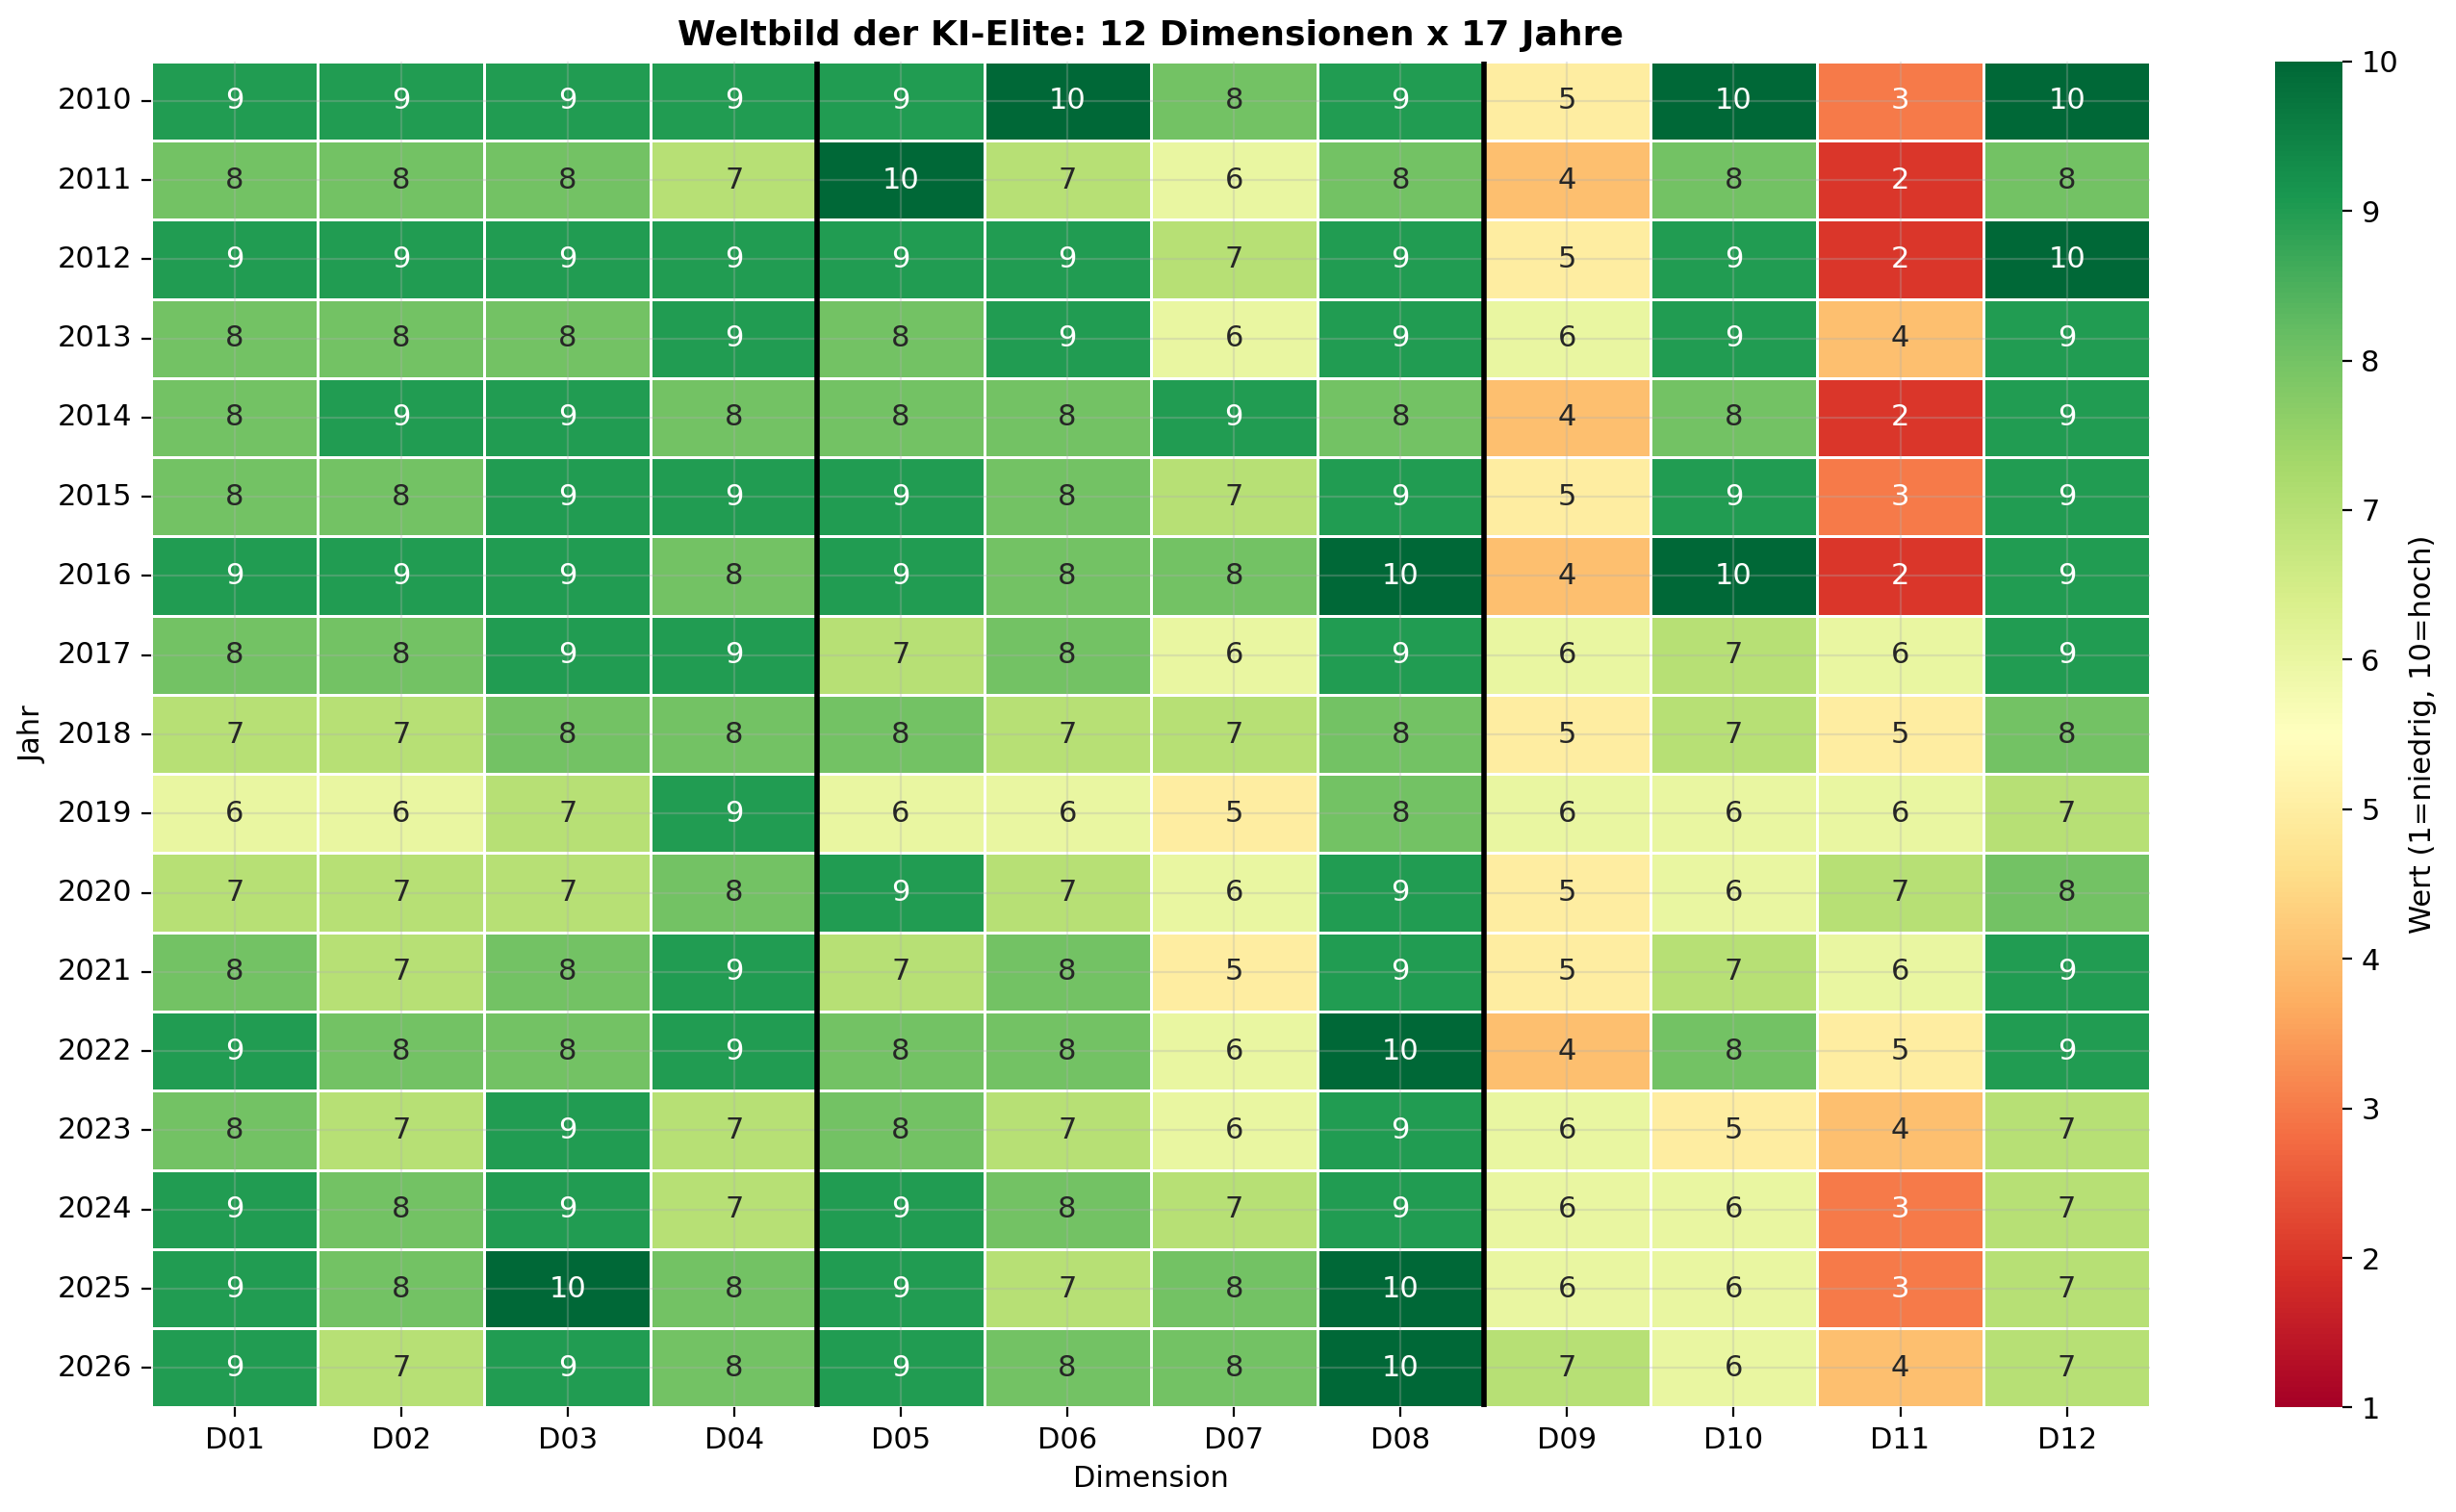
\includegraphics[width=0.95\textwidth]{fig2_heatmap.png}
  \caption{Heatmap der 12 Weltbild-Dimensionen \"uber alle untersuchten Gruppen. Hohe Werte (dunkel) markieren intensive \"Uberzeugungen; die Doppelsenke bei D09 und D11 ist \"uber alle Gruppen hinweg sichtbar.}
  \label{fig:heatmap}
\end{figure}


\subsubsection{Das Weltbild der Top~10}

Die zehn m\"achtigsten KI-Akteure vertreten dasselbe Weltbild in intensivierter Form (Avg~7,7). Auf zehn von zw\"olf Dimensionen liegen die Top-10-Werte exakt einen Skalenpunkt \"uber dem Kollektiv. Die beiden Ausnahmen: Menschenfreundlichkeit (D09=4) und Egalitarismus (D11=4) liegen \emph{niedriger}. Je m\"achtiger die Position, desto ausgepr\"agter das Sendungsbewusstsein und desto distanzierter das Menschenbild.


\subsubsection{Kern\"uberzeugungen}

Die Destillation der am h\"aufigsten wiederholten Aussagen (SE~5: HOM\_haeuf\_A, vgl.\ Anhang~\ref{app:se}) identifiziert f\"unf \"Uberzeugungen als Minimalkonsens: (1)~Technologie als moralisches Gebot, (2)~Elite-Steuerung, (3)~das Befreiungsnarrativ, (4)~geopolitischer Manich\"aismus, (5)~Arbeit als Identit\"at. Sicherheitsrhetorik geh\"ort zum Kernbestand des Diskurses, fungiert aber als diskursive Ressource, nicht als handlungsleitende \"Uberzeugung.

\medskip
\noindent\textbf{Kernbefund F1:} Die rekonstruierten Profile deuten auf ein koh\"arentes, hochintensives \"Uberzeugungssystem hin, das sich als \emph{technologischer Messianismus mit Ambivalenzstruktur} charakterisieren l\"asst. Die Bezeichnung \glqq Messianismus\grqq{} ist dabei als idealtypische Zuspitzung zu verstehen, nicht als psychologische Diagnose: Sie bezeichnet die spezifische \emph{Kombination} aus hohem Sendungsbewusstsein (D01), Techno-Determinismus (D05), Dringlichkeit (D08) und geringer anthropologischer Wertsch\"atzung (D09) -- ein Profil, das \"uber blo\ss{}es Sendungsbewusstsein hinausgeht, weil es technologischen Fortschritt als quasi-erl\"oserische Notwendigkeit rahmt.


\subsection{F2 -- Wandel des Weltbilds (l\"angsschnittlich)}
\label{sec:ergebnisse:f2}

\subsubsection{Entwicklung der 12 Dimensionen \"uber die Zeit}

Von zw\"olf Dimensionen zeigen vier ausgepr\"agte lineare Trends (Tabelle~\ref{tab:trends}).\footnote{Die hier berichteten Trendlinien beschreiben \textit{Muster in rekonstruierten Daten}: Die Weltbild-Werte sind LLM-gest\"utzte Rekonstruktionen, keine unabh\"angigen Messungen. OLS-Steigungen und $R^2$ dienen der Beschreibung der Verlaufsmuster, nicht der inferenzstatistischen Hypothesenpr\"ufung. Eine externe Validierung (Expertenratings vs.\ SWR-Output) steht noch aus (vgl.\ Abschnitt Limitations).}

\begin{table}[htbp]
  \centering
  \caption{Ausgepr\"agte lineare Trends (OLS-Beschreibung, $n=17$ Jahrespunkte).}
  \label{tab:trends}
  \begin{tabular}{l l c c}
    \toprule
    \textbf{Dimension} & \textbf{Richtung} & \textbf{Steigung/Dekade} & $R^2$ \\
    \midrule
    D10 Posthumanismus       & fallend  & $-2{,}4$ & $0{,}63$ \\
    D12 Kontroll\"uberzeugung & fallend  & $-1{,}5$ & $0{,}54$ \\
    D02 Selbstwirksamkeit    & fallend  & $-1{,}0$ & $0{,}31$ \\
    D09 Menschenfreundlichkeit & steigend & $+0{,}9$ & $0{,}27$ \\
    \bottomrule
  \end{tabular}
\end{table}

Den st\"arksten R\"uckgang verzeichnet der Posthumanismus (D10): von 10 im Jahr 2010 auf 6 im Jahr 2025. Die hohe Pearson-Korrelation mit D12 ($r = +0{,}85$)\footnote{Die hier und im Folgenden berichteten Korrelationen (Pearson, berechnet \"uber die 17~Jahreszeitpunkte) sind \emph{Zusammenh\"ange innerhalb der LLM-Rekonstruktion}, nicht zwischen unabh\"angig gemessenen Variablen. Sie k\"onnten interne Koh\"arenz des Modells widerspiegeln statt empirischer Zusammenh\"ange in der Realit\"at (vgl.\ Abschnitt~\ref{sec:limitationen}).} weist auf ein zusammenh\"angendes Ph\"anomen: Posthumanismus und Kontroll\"uberzeugung erodieren synchron. Der einzige deutlich steigende Wert betrifft die Menschenfreundlichkeit (D09), wobei die negative Korrelation mit D10 ($r = -0{,}58$) eine kompensatorische Verkn\"upfung nahelegt. Der Gesamtdurchschnitt bleibt nahezu konstant (Fr\"uhphase 7,5, Sp\"atphase 7,3), was eine tektonische Verschiebung unter der Oberfl\"ache verbirgt.

\begin{figure}[htbp]
  \centering
  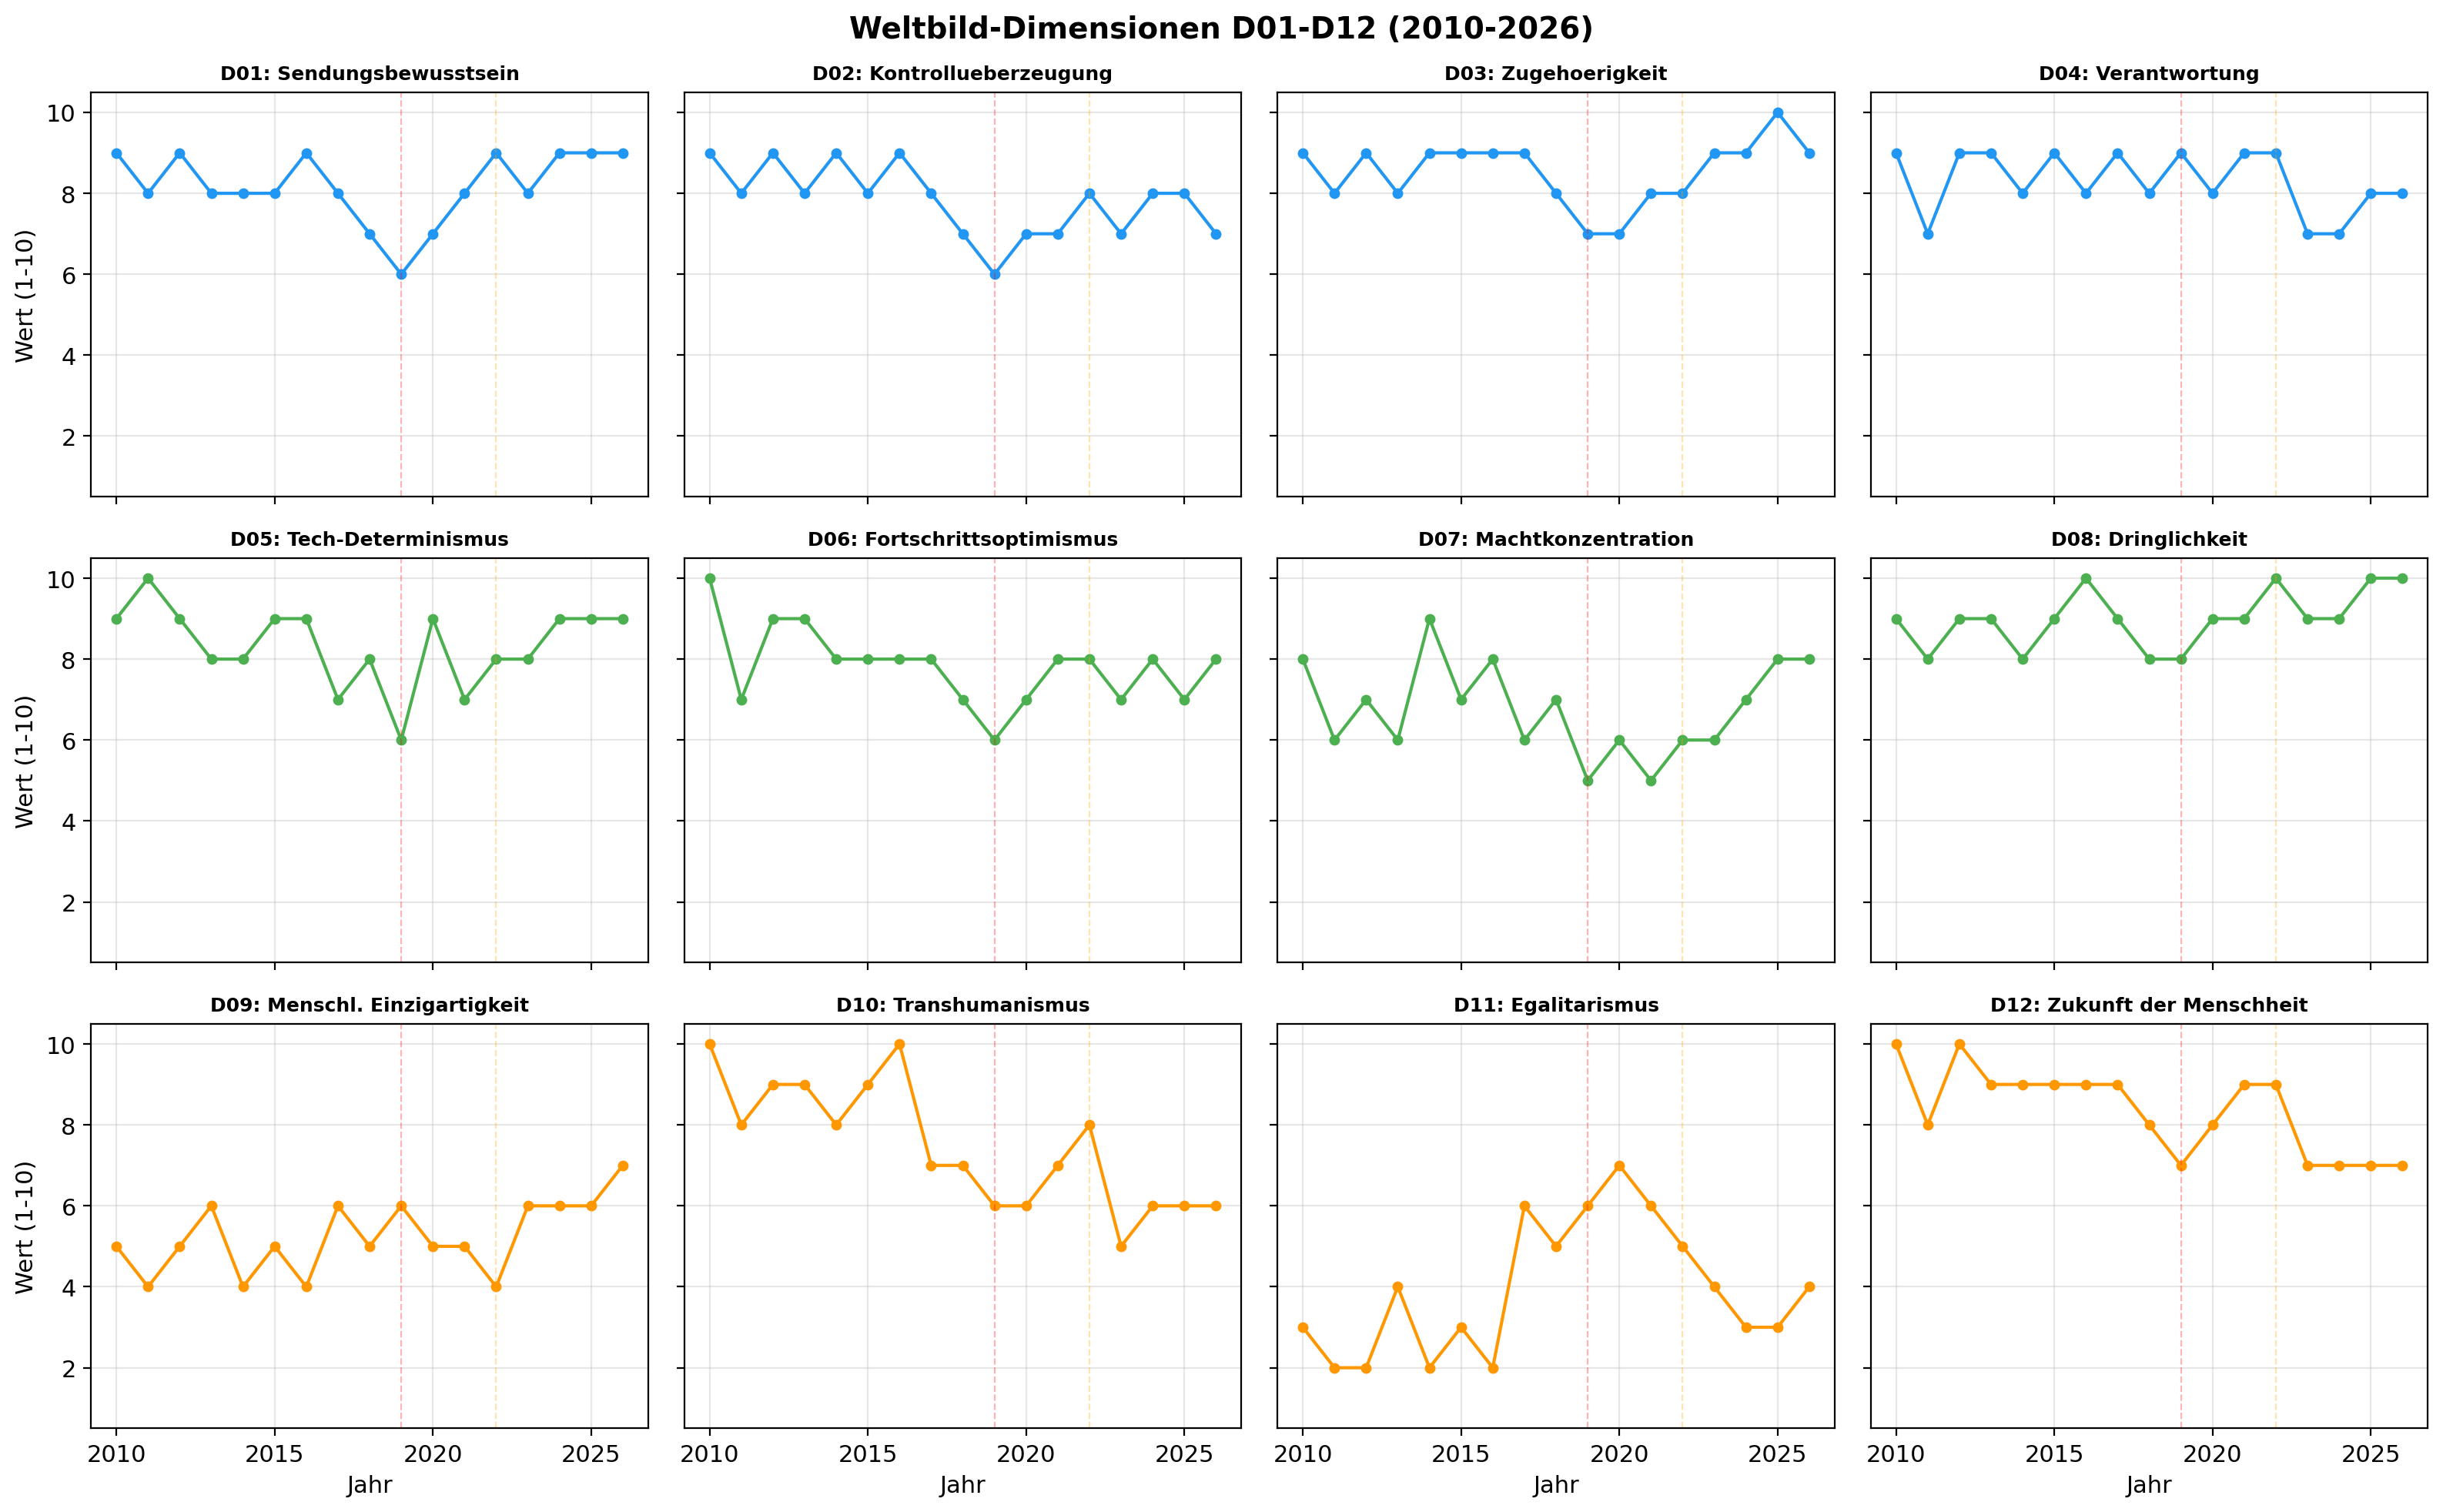
\includegraphics[width=\textwidth]{fig1_zeitreihen_panel.png}
  \caption{Zeitreihen der 12 Weltbild-Dimensionen (2010--2026). Ausgepr\"agte Trends sind hervorgehoben. Der markante Abfall von D10 (Posthumanismus) und D12 (Kontroll\"uberzeugung) bildet den \glqq Utopie-Komplex\grqq, dessen Zerfall durch steigende Dringlichkeit (D08) arithmetisch kompensiert wird.}
  \label{fig:zeitreihen}
\end{figure}

\begin{figure}[htbp]
  \centering
  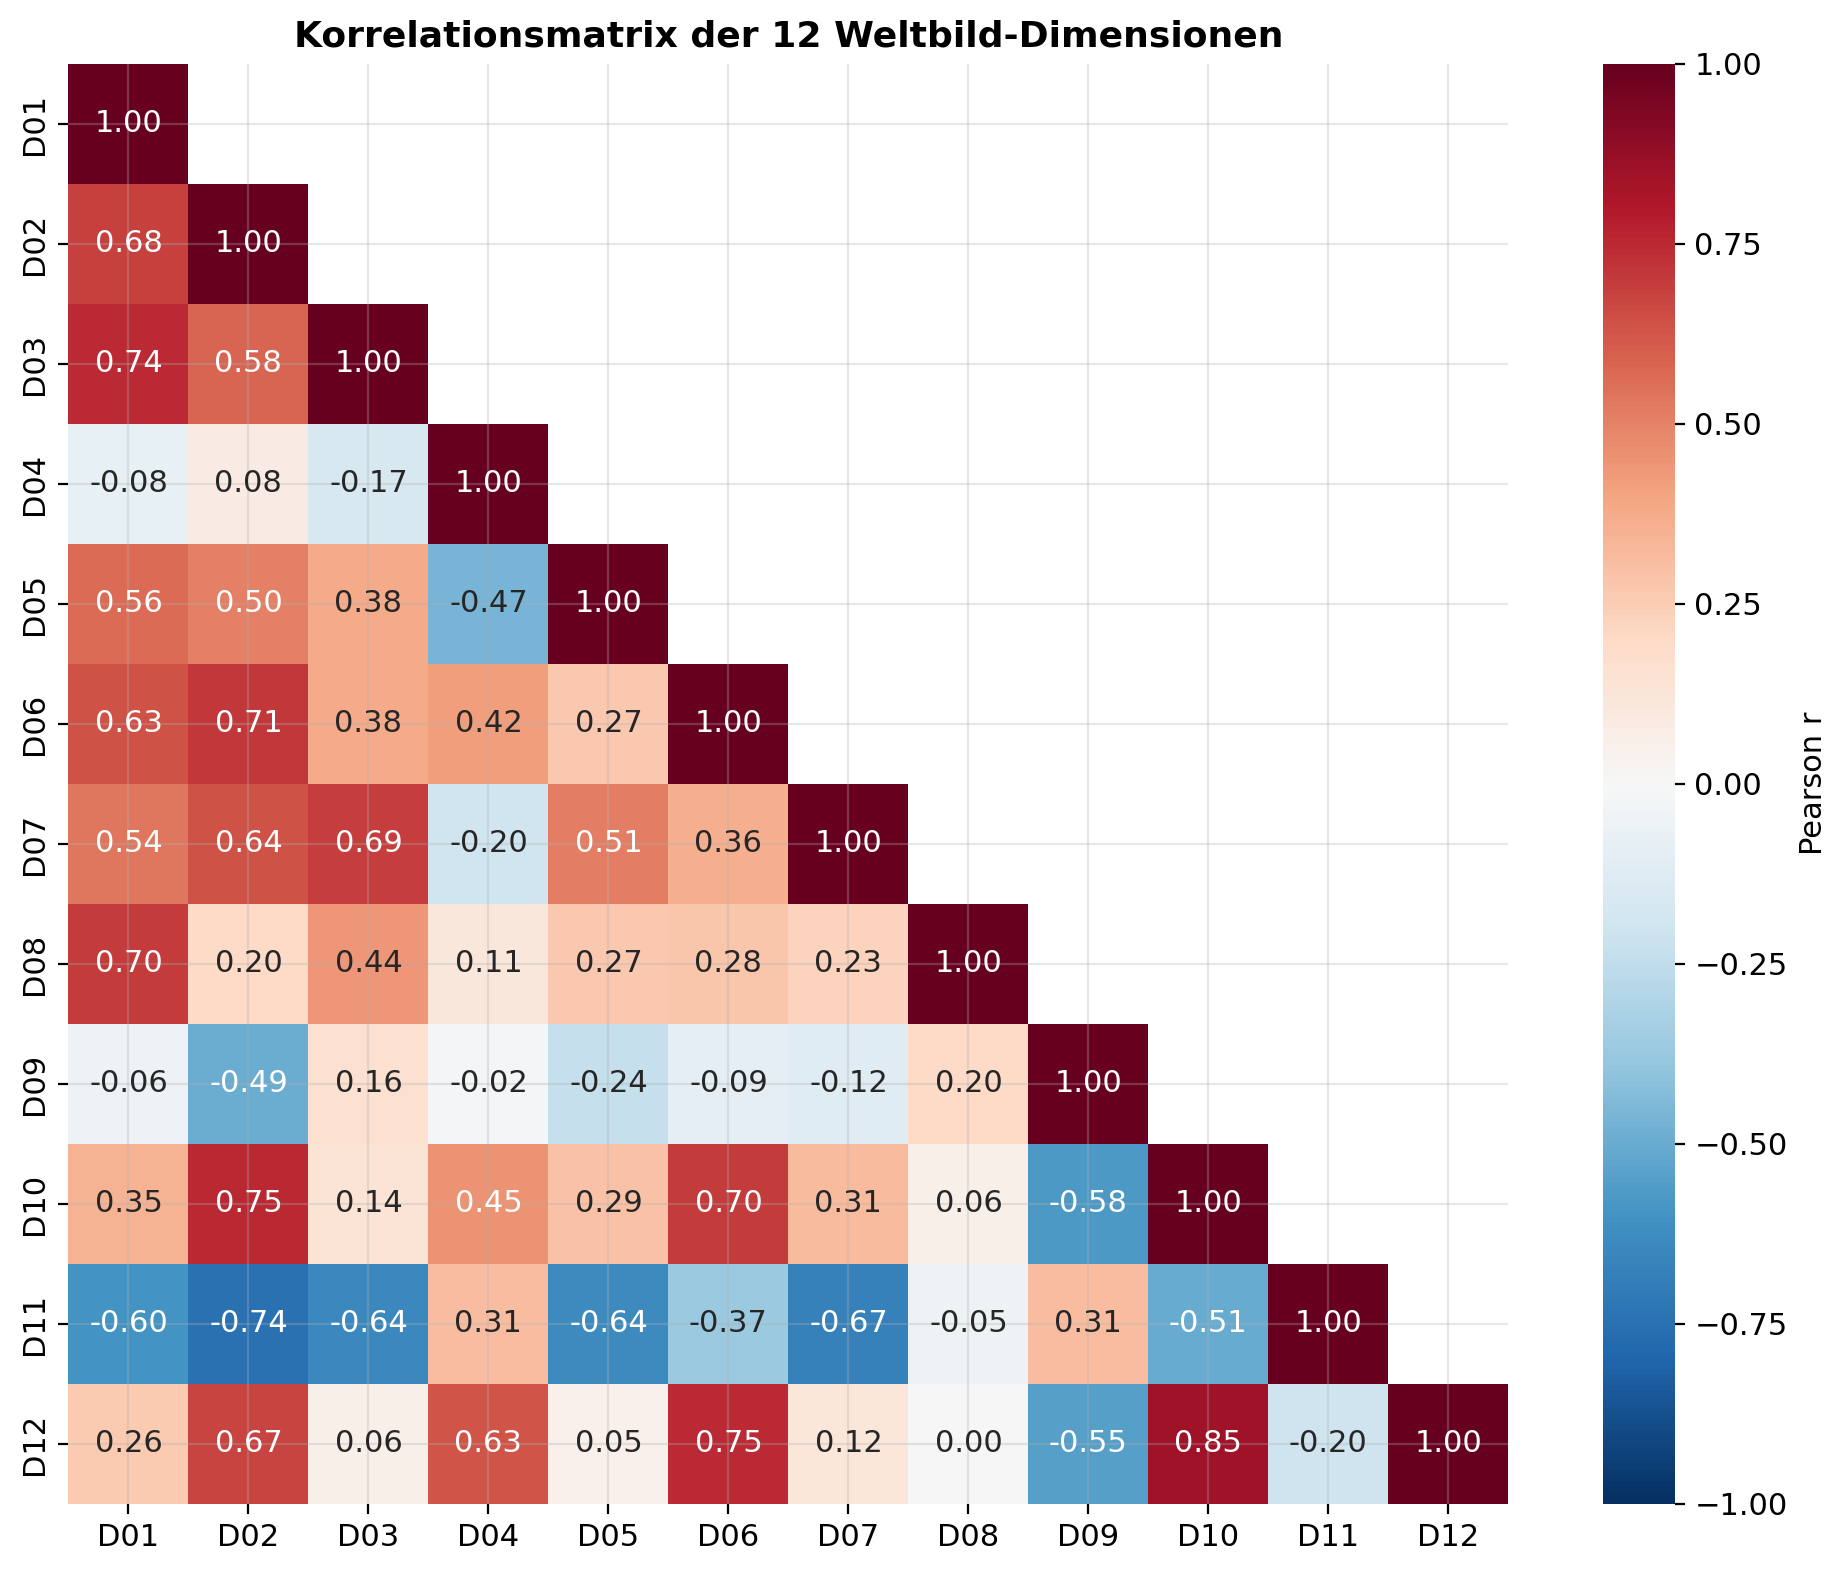
\includegraphics[width=0.85\textwidth]{fig4_korrelationsmatrix.png}
  \caption{Korrelationsmatrix der 12 Dimensionen. Die starke positive Korrelation zwischen D10 und D12 sowie die negative Korrelation zwischen D10 und D09 bilden den empirischen Kern des \glqq Utopie-Komplexes\grqq.}
  \label{fig:korrelationsmatrix}
\end{figure}


\subsubsection{Wendepunkte und Epochenvergleich}

Die Breakpoint-Detection -- durchgef\"uhrt als visuelle Inspektion der Zeitreihen, erg\"anzt durch die Identifikation synchroner Extrempunkte \"uber mehrere Dimensionen -- identifiziert zwei zentrale Wendepunkte.\footnote{Eine formale Breakpoint-Analyse (z.\,B.\ Bai-Perron-Test) war aufgrund der geringen Zahl von Zeitpunkten ($n=17$) und der Natur der Daten (LLM-Rekonstruktionen, keine unabh\"angigen Messungen) nicht sinnvoll anwendbar. Die Wendepunkte sind daher als \emph{deskriptive Beobachtungen} zu verstehen, nicht als statistisch gesicherte Strukturbr\"uche.} Der erste liegt bei 2019: Vier Dimensionen (D01, D02, D05, D06) erreichen synchron ihren Tiefpunkt, zeitlich assoziiert mit der GPT-2-Zur\"uckhaltung. Der zweite, dauerhaftere Wendepunkt liegt bei 2022/2023: Zeitgleich mit der ChatGPT-Ver\"offentlichung zeigt sich ein markanter Musterwechsel -- Dringlichkeit erreicht ihr rekonstruiertes Maximum (D08=10), Egalitarismus f\"allt von 6 auf 4. Im Unterschied zu 2019 kehren die Werte nicht zur\"uck; die rekonstruierten Profile nach 2022 deuten auf ein neues Gleichgewicht hin. Dabei ist zu beachten, dass die identifizierten Wendepunkte nicht isoliert von breiteren gesellschaftlichen Entwicklungen zu sehen sind: Die COVID-19-Pandemie (2020--2022) hat die Digitalisierungsdynamik beschleunigt und d\"urfte das Dringlichkeitserleben verst\"arkt haben; die zunehmende geopolitische Polarisierung (US-China-Technologiekonflikt) hat den \glqq manich\"aischen\grqq{} Aspekt des Weltbilds m\"oglicherweise befeuert; und der Beginn regulatorischer Initiativen (EU~AI~Act, 2021ff.) hat die Debatte um Governance versch\"arft. Diese Kontextfaktoren lassen sich mit der vorliegenden Methode nicht vom KI-spezifischen Wandel trennen.

\begin{figure}[htbp]
  \centering
  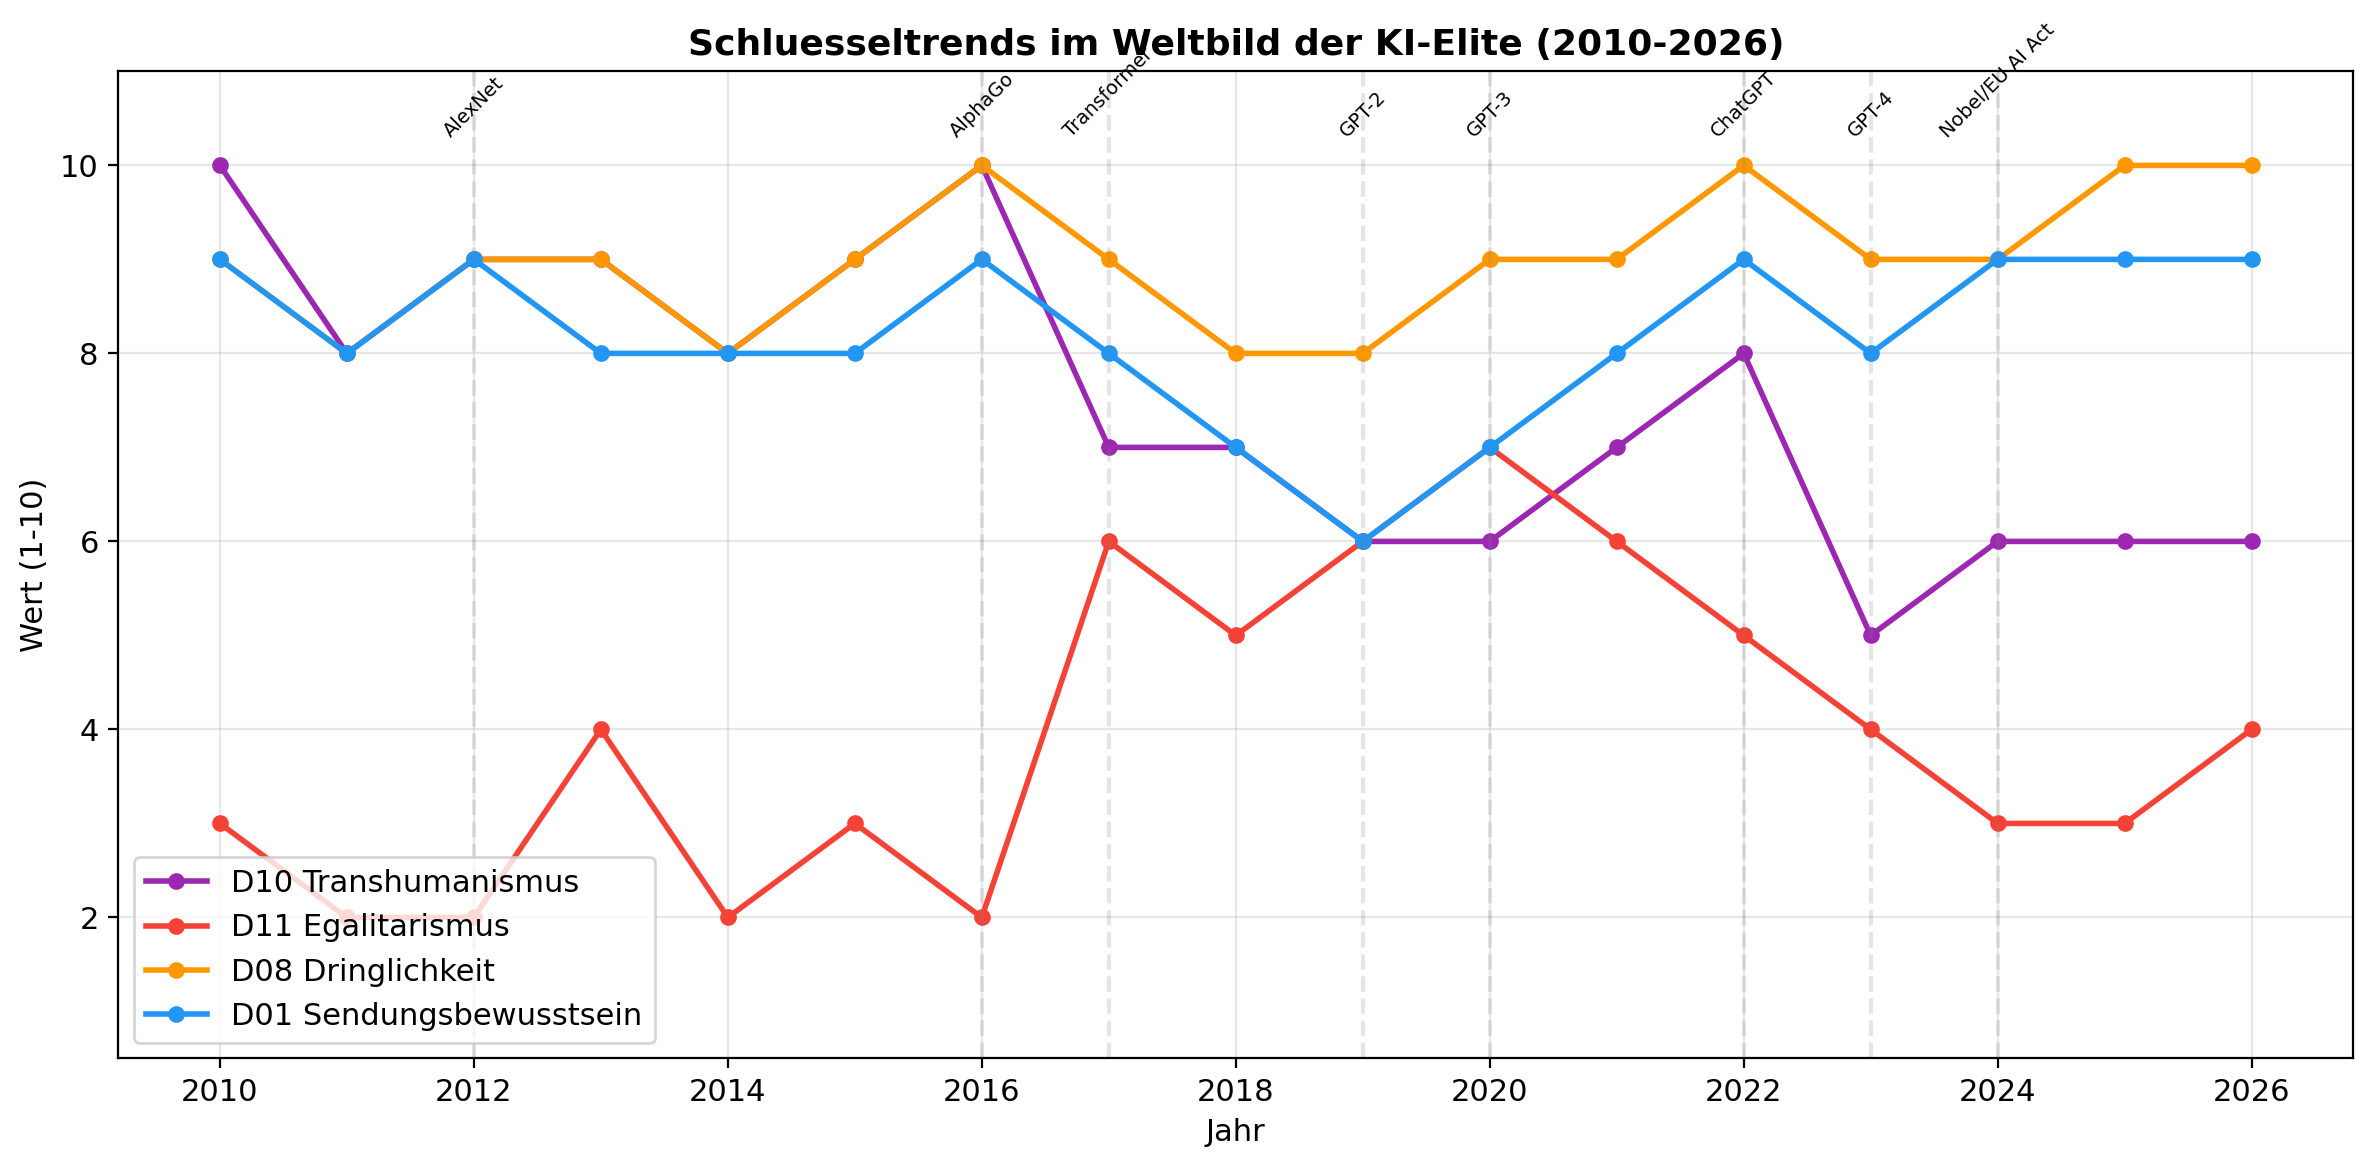
\includegraphics[width=0.95\textwidth]{fig7_schluesseltrends.png}
  \caption{Schl\"usseltrends der Weltbild-Transformation. Die zwei Wendepunkte (2019, 2022/2023) und die drei Epochen (Prometheischer Optimismus, Erste Ambivalenz, Tragisches Bewusstsein) sind markiert.}
  \label{fig:schluesseltrends}
\end{figure}


\subsubsection{Konvergenz oder Divergenz?}

Die Daten zeigen eine zunehmende Ausdifferenzierung. Der ChatGPT-Effekt intensiviert sowohl die Architekten-Position (Beschleunigung, Machtkonzentration) als auch die H\"uter-Position (Vorsicht, Regulierung) gleichzeitig -- er wirkt als Katalysator der Bipolarisierung.


\subsubsection{Metaphern- und Emotions-Wandel}

Die Leitmetapher verschiebt sich von Prometheus -- dem Feuerbringer -- zum tragischen Helden, der retten muss, was m\"oglicherweise nicht mehr zu retten ist. Die Handlung bleibt dieselbe (Beschleunigung), aber ihre emotionale Rahmung dreht sich um: nicht mehr aus Euphorie, sondern aus dem Glauben, dass die Alternative schlimmer w\"are.

\medskip
\noindent\textbf{Kernbefund F2:} Die rekonstruierten Profile deuten auf eine strukturelle Transformation des Weltbilds hin -- von einer monochromen Utopie zu einer bimodalen Wette. \emph{Tragisch} im Sinne der Bezeichnung \glqq tragischer Beschleunigungszwang\grqq{} meint die gleichzeitige Erosion utopischer Gewissheiten und Persistenz der Handlungsrichtung: Die Akteure beschleunigen, obwohl sie an der Zukunft zweifeln, die sie bauen -- weil sie die Alternativen (geopolitischer R\"uckfall, Kontrollverlust an weniger verantwortungsvolle Akteure) als schlimmer bewerten. Drei Erosionstrends (D10, D12, D02) bilden einen \glqq Utopie-Komplex\grqq, dessen Zerfall durch steigende Dringlichkeit (D08) arithmetisch kompensiert wird. Allerdings ist nicht auszuschlie\ss{}en, dass der R\"uckgang des Posthumanismus (D10) teilweise ein Artefakt ver\"anderter \"offentlicher Diskurse ist: Wenn das Thema medial weniger pr\"asent ist, sinkt auch die Datendichte entsprechender Aussagen, was die LLM-Rekonstruktion verzerren kann.


\subsection{F3 -- Kongruenz von Aussagen und Handlungen}
\label{sec:ergebnisse:f3}

\begin{table}[htbp]
  \centering
  \caption{Vergleich Aussagen (A) und Handlungen (H), $N=100$.}
  \label{tab:kongruenz}
  \begin{tabular}{l c c c l}
    \toprule
    \textbf{Dimension} & \textbf{Sagen} & \textbf{Handeln} & $\Delta$ & \textbf{Urteil} \\
    \midrule
    D01 Sendungsbewusstsein     & 8 & 7 & $-1$ & Leicht \\
    D02 Selbstwirksamkeit       & 8 & 9 & $+1$ & Handeln $>$ Sagen \\
    D03 Arbeitsethos            & 8 & 9 & $+1$ & Handeln $>$ Sagen \\
    D04 Verantwortungsgef\"uhl  & 7 & 5 & $\mathbf{-2}$ & Stark \\
    D05 Techno-Determinismus    & 8 & 9 & $+1$ & Handeln $>$ Sagen \\
    D06 Fortschrittsglaube      & 8 & 6 & $\mathbf{-2}$ & Stark \\
    D07 Machtkonzentration      & 6 & 8 & $\mathbf{+2}$ & Stark \\
    D08 Dringlichkeit           & 8 & 9 & $+1$ & Handeln $>$ Sagen \\
    D09 Menschenfreundlichkeit  & 5 & 3 & $\mathbf{-2}$ & Stark \\
    D10 Posthumanismus          & 7 & 8 & $+1$ & Handeln $>$ Sagen \\
    D11 Egalitarismus           & 5 & 2 & $\mathbf{-3}$ & \textbf{Sehr gro\ss{}} \\
    D12 Kontroll\"uberzeugung   & 8 & 7 & $-1$ & Leicht \\
    \midrule
    \textbf{Durchschnitt}       & \textbf{7,2} & \textbf{6,8} & $-0{,}4$ & \\
    \bottomrule
  \end{tabular}
\end{table}

Methodisch ist zu beachten, dass beide Profile -- Aussagen wie Handlungen -- als \emph{Textbeschreibungen} in das LLM eingehen; das Modell verarbeitet nicht Handlungen selbst, sondern deren sprachliche Kodierung. Die Diskrepanzen ordnen sich in zwei komplement\"are Cluster. Das \emph{Abw\"arts-Cluster} (Handeln $<$ Sagen) umfasst die gesellschaftsorientierten Dimensionen: Egalitarismus ($\Delta\,-3$), Verantwortungsgef\"uhl, Fortschrittsglaube und Menschenfreundlichkeit (je $\Delta\,-2$). Das \emph{Aufw\"arts-Cluster} (Handeln $>$ Sagen) umfasst die machtbezogenen Dimensionen: Machtkonzentration ($\Delta\,+2$), Selbstwirksamkeit, Arbeitsethos, Techno-Determinismus (je $\Delta\,+1$). Das resultierende Muster: eine systematische Selbstdarstellungs-Asymmetrie. \"Offentlich pr\"asentiert sich die KI-Elite gem\"a\ss{}igter, verantwortungsvoller und egalit\"arer, als sie in der Praxis agiert.

\begin{figure}[htbp]
  \centering
  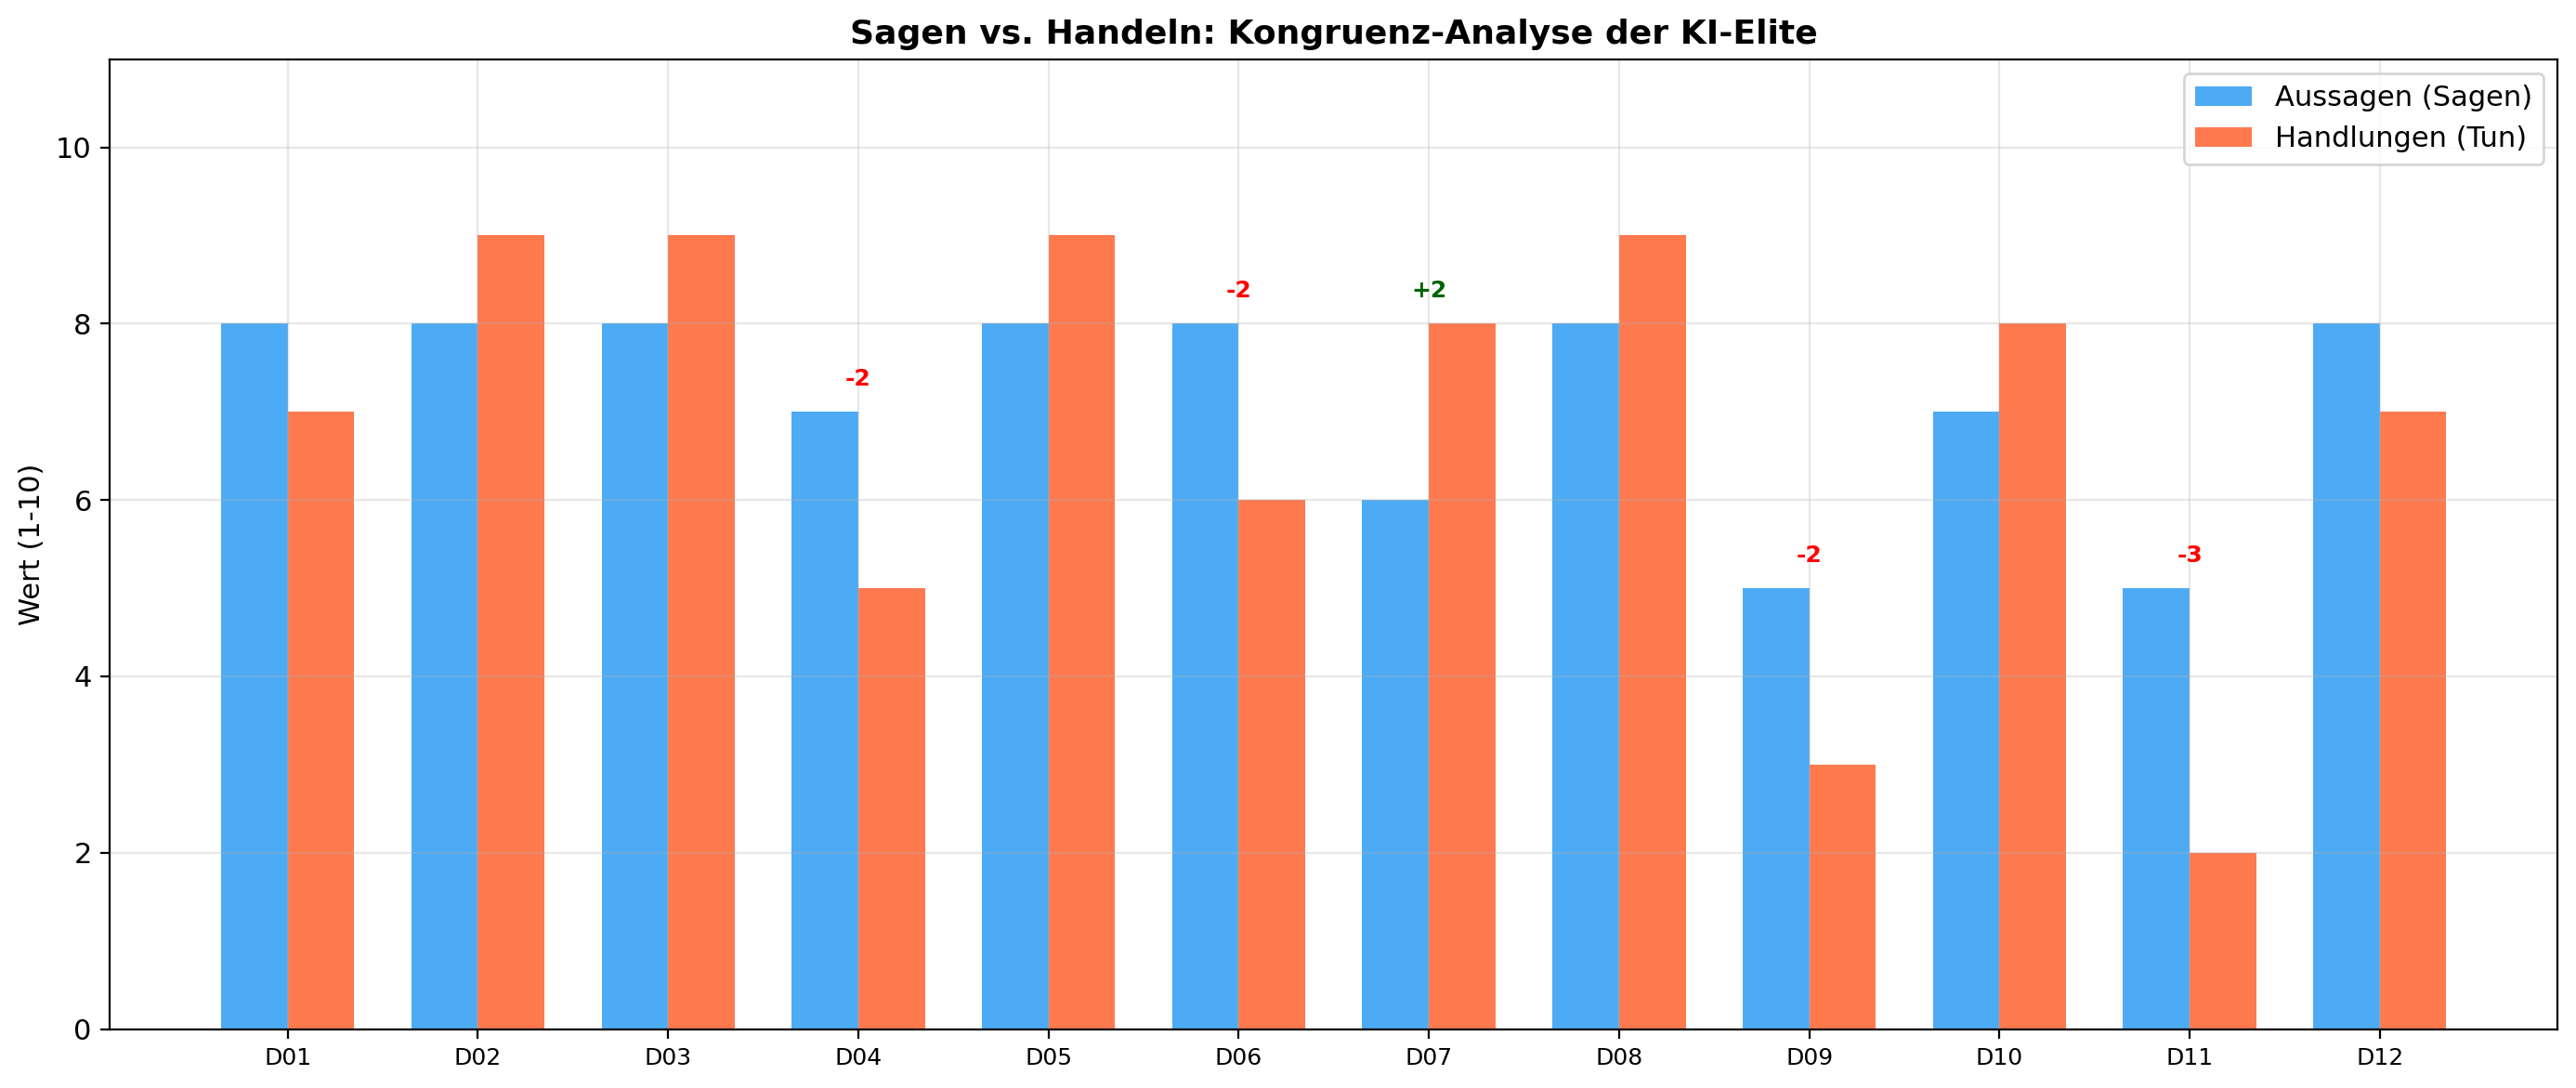
\includegraphics[width=0.95\textwidth]{fig6_sagen_vs_handeln.png}
  \caption{Sagen vs.\ Handeln: Vergleich der aus Aussagen (A) und Handlungen (H) rekonstruierten Weltbilder. Die gesellschaftsorientierten Dimensionen (D04, D06, D09, D11) fallen im Handeln systematisch ab, w\"ahrend die machtbezogenen Dimensionen (D07, D05) im Handeln steigen.}
  \label{fig:sagen_handeln}
\end{figure}

Die gr\"o\ss{}te Einzeldiskrepanz ($\Delta\,-3$ bei D11) zeigt: In Aussagen spricht die KI-Elite von \glqq Zugang f\"ur alle\grqq; in ihren Handlungen baut sie Mehrfach-Stimmrechtsaktien, konzentriert Compute-Infrastruktur und schafft exklusive Netzwerke. Zur Einordnung: Ein $\Delta$ von 3 auf einer 10-Punkte-Skala entspricht knapp einem Drittel der gesamten Skalenbreite -- ein Unterschied, der bei inhaltlicher Interpretation als substanziell zu werten ist.\footnote{Eine formale Effektst\"arkeberechnung (z.\,B.\ Cohen's $d$) ist hier nicht m\"oglich, da keine Individualebene-Streuungsma\ss{}e vorliegen. Die Einordnung als \glqq gro\ss{}\grqq{} basiert auf der inhaltlichen Interpretation der Skalenbreite, nicht auf psychometrischen Konventionen.}

\medskip
\noindent\textbf{Kernbefund F3:} Die rekonstruierten Profile zeigen eine systematische, gerichtete Diskrepanz zwischen Aussagen- und Handlungsprofilen. Dieses Muster ist konsistent mit der Hypothese einer funktionalen Inkongruenz, muss aber vor dem Hintergrund des Erwarteten-Diskrepanz-Bias (vgl.\ Abschnitt~\ref{sec:limitationen}) mit Vorsicht interpretiert werden: LLMs k\"onnten die in der sozialwissenschaftlichen Literatur dokumentierte Sagen-Handeln-Kluft bei Eliten reproduzieren, anstatt sie empirisch zu entdecken.


\subsection{F4 -- Weltbild-Cluster}
\label{sec:ergebnisse:f4}

Aus den Daten lassen sich vier distinkte Weltbild-Typen identifizieren (Tabelle~\ref{tab:typen}).

\textbf{Identifikationsmethode:} Die Cluster-Identifikation erfolgte in einem zweistufigen Verfahren. \emph{Stufe~1 (LLM-gest\"utzt):} Alle 15 Gruppen-Synthesen wurden nach \"Ahnlichkeitsmustern in den 12~Dimensionen gruppiert, wobei die gr\"o\ss{}ten Varianzachsen (D07~Machtkonzentration, D09~Menschenfreundlichkeit, D11~Egalitarismus) als Trennmerkmale fungierten. \emph{Stufe~2 (Autor-Validierung):} Die vom LLM vorgeschlagene Vier-Cluster-L\"osung wurde vom Autor anhand inhaltlicher Koh\"arenz und Plausibilit\"at evaluiert. Alternative L\"osungen (drei und f\"unf Cluster) wurden gepr\"uft und verworfen: Drei Cluster verschmelzen Innovator und Befreier, was inhaltlich nicht gerechtfertigt ist; f\"unf Cluster spalten den H\"uter-Typ in eine Untergruppe, die empirisch nicht stabil reproduziert werden konnte. Wir betonen, dass diese Cluster-Identifikation \emph{explorativ} ist -- eine konfirmatorische Validierung an einem unabh\"angigen Datensatz steht aus. Die Cluster-L\"osung ist eine \emph{interpretative Hypothese}, nicht ein statistisch abgesichertes Ergebnis im Sinne formaler Clusteranalyse.

\begin{table}[htbp]
  \centering
  \caption{Die vier Weltbild-Typen der KI-Elite. Die Werte sind Cluster-Durchschnitte aus den Gruppen-Synthesen; individuelle Abweichungen innerhalb eines Clusters k\"onnen erheblich sein (vgl.\ die Andreessen-Diskrepanz in der nachfolgenden Fu\ss{}note).}
  \label{tab:typen}
  \small
  \begin{tabular}{l c c c c}
    \toprule
    \textbf{Merkmal} & \textbf{I \glqq Architekt\grqq} & \textbf{II \glqq H\"uter\grqq} & \textbf{III \glqq Innovator\grqq} & \textbf{IV \glqq Befreier\grqq} \\
    \midrule
    $n$ & 35 & 25 & 22 & 18 \\
    Prototyp & CEOs, Investoren & Akademiker, Risiko-W. & Gr\"under & Open Source \\
    Avg D01--D12 & 7,8 & 6,4 & 7,2 & 6,8 \\
    D04 Verantwortung & 6,3 & \textbf{9,0} & 8,3 & 6,0 \\
    D07 Machtkonzentr. & \textbf{8,8} & 4,8 & 6,5 & \textbf{2,5} \\
    D09 Menschenfreundl. & \textbf{3,3} & 5,8 & 4,8 & \textbf{6,5} \\
    D11 Egalitarismus & \textbf{2,8} & \textbf{7,2} & 5,0 & \textbf{7,5} \\
    \bottomrule
  \end{tabular}
\end{table}

Der \textbf{Architekt} vereint maximales Sendungsbewusstsein mit minimalem Egalitarismus: Machtkonzentration ist Voraussetzung f\"ur Handlungsf\"ahigkeit. Der \textbf{H\"uter} bildet den Gegenpol: maximale Verantwortung, Forderung nach institutioneller Begrenzung. Der \textbf{Innovator} steht dazwischen. Der \textbf{Befreier} ist die \"uberraschendste Entdeckung: minimale Machtkonzentration \emph{und} hoher Egalitarismus -- Regulierungsgegner, die Macht radikaler verteilen wollen als alle anderen, allerdings durch M\"arkte und Open-Source-Communities.\footnote{Der hohe D11-Wert des Befreier-Typs (7,5) und der niedrige D11-Wert einzelner Prototypen (z.\,B.\ Andreessen: D11=2) markieren eine Konstruktvalidit\"atsproblem: D11 misst Gleichheitsorientierung, nicht deren \emph{Mechanismus}. Marktlibertaerer Zugangs-Egalitarismus (Befreier) und redistributiver Egalitarismus (H\"uter) produzieren \"ahnliche Skalenwerte auf D11, meinen aber Verschiedenes. Der Prototyp-Wert bezieht sich auf die Einzelperson-Synthese, der Cluster-Wert auf das Gruppenaggregat -- Andreessens individuelles Profil weicht vom Cluster-Durchschnitt ab. K\"unftige Operationalisierungen sollten hier differenzieren.}

\begin{figure}[htbp]
  \centering
  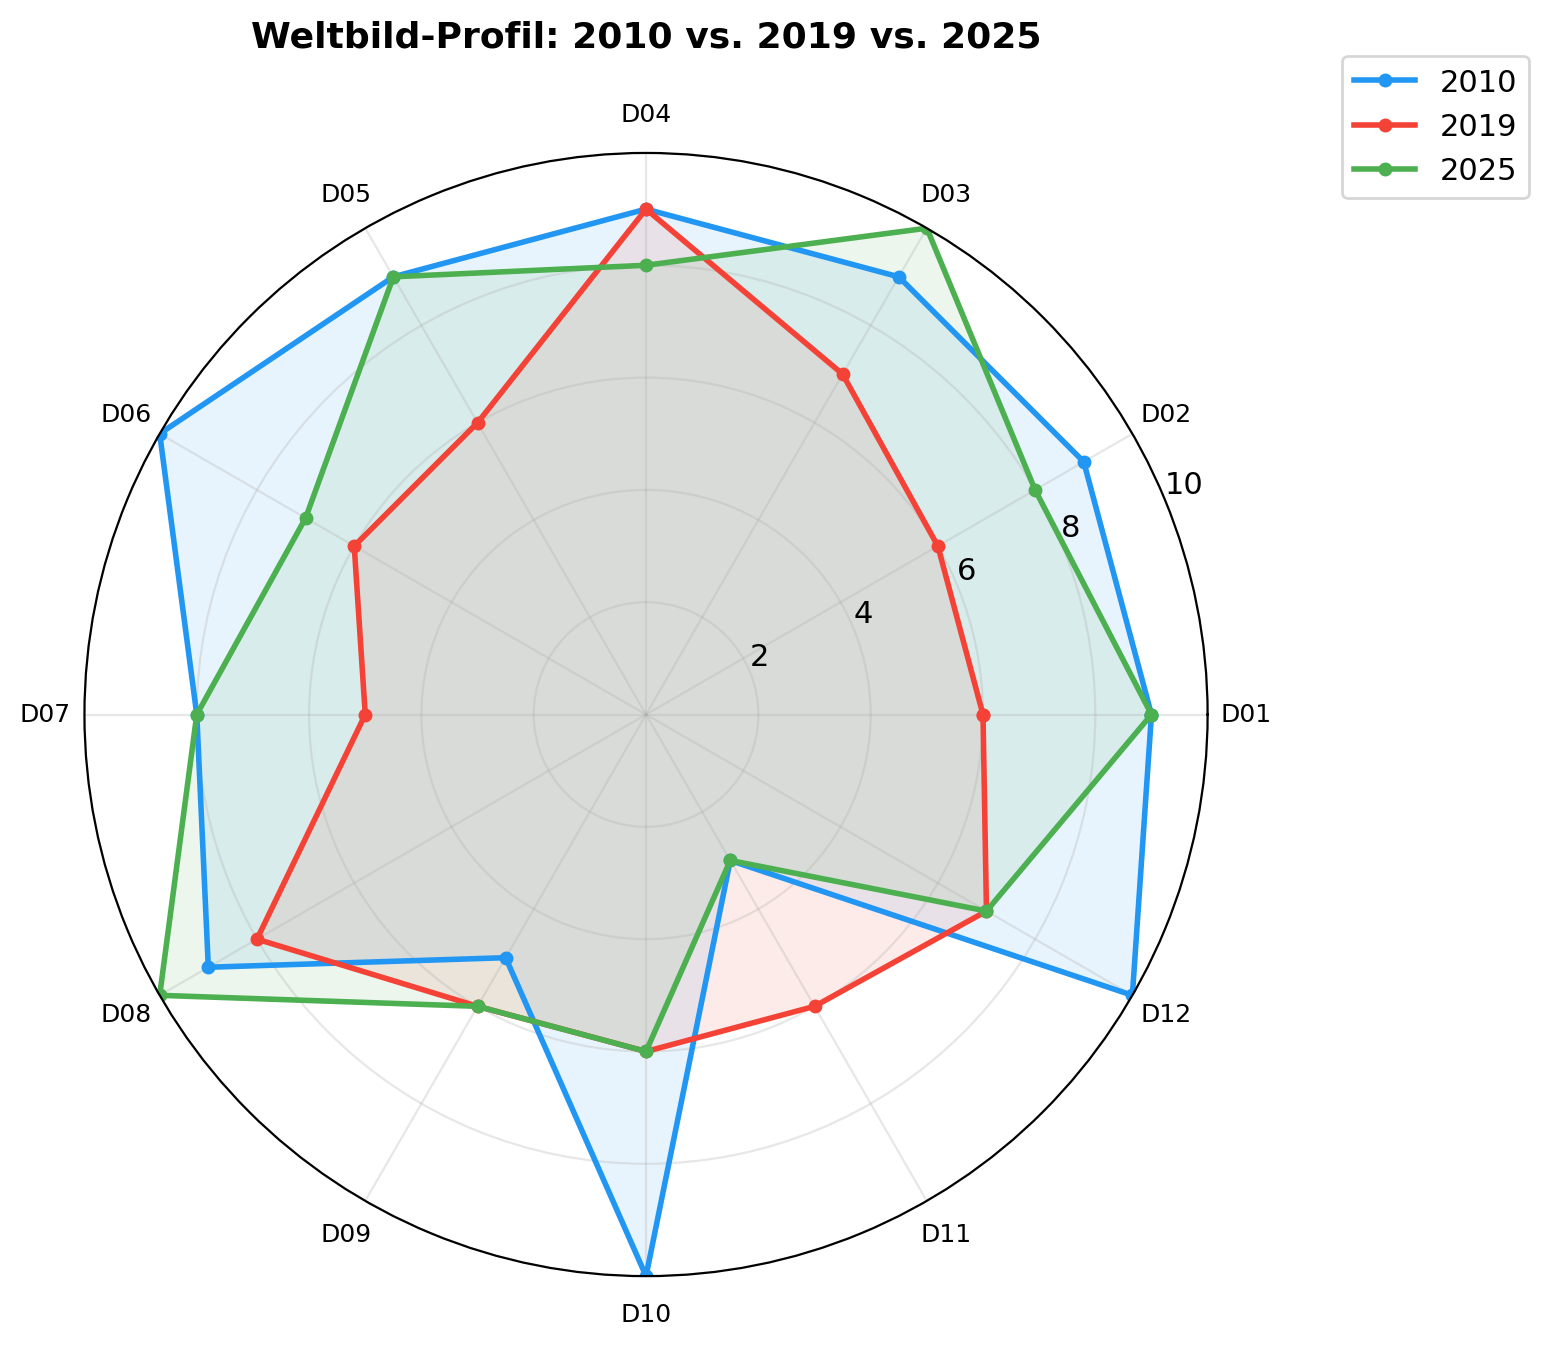
\includegraphics[width=0.85\textwidth]{fig3_radar_vergleich.png}
  \caption{Radar-Diagramm der vier Weltbild-Typen auf den 12 Dimensionen. Die Polarisierung zwischen Architekt (au\ss{}en) und H\"uter (innen) sowie die distinkte Position des Befreiers (hoher Egalitarismus bei niedriger Machtkonzentration) sind sichtbar.}
  \label{fig:radar}
\end{figure}

\medskip
\noindent\textbf{Kernbefund F4:} Die st\"arkste Polarisierung besteht zwischen Typ~I (Herrschaftslogik) und Typ~II (Teilhabelogik). Die explorative Vier-Cluster-L\"osung bedarf einer konfirmatorischen Validierung an unabh\"angigen Daten, bevor sie als robustes Ergebnis gelten kann.


\subsection{F5 -- Subgruppenvergleiche}
\label{sec:ergebnisse:f5}

\begin{table}[htbp]
  \centering
  \caption{Ranking der Subgruppen-Differenzen. $\Delta$ = Gr.~1 $-$ Gr.~2 (Durchschnitt); Einzelkontraste beziehen sich auf die Dimension mit der gr\"o\ss{}ten Abweichung.}
  \label{tab:subgruppen}
  \small
  \begin{tabular}{c l c c c l}
    \toprule
    \textbf{Rang} & \textbf{Vergleich} & \textbf{Avg Gr.~1} & \textbf{Avg Gr.~2} & $\Delta$ & \textbf{St\"arkster Kontrast} \\
    \midrule
    1 & Risiko vs.\ Speed   & 5,9 & 7,6 & 1,7 & D02, D06, D10, D12: je $-5$ \\
    2 & CEOs vs.\ Akademiker & 7,8 & 6,3 & 1,5 & D07: $+4$, D11: $-4$ \\
    3 & Frauen vs.\ M\"anner & 6,9 & 8,1 & 1,2 & D11: $-6$ \\
    4 & Open vs.\ Closed     & 6,8 & 6,3 & 0,5 & D07: $-3$, D12: $+3$ \\
    5 & Reg-Pro vs.\ Contra  & 6,3 & 6,8 & 0,5 & D04: $+4$, D06: $-3$ \\
    6 & Anthropic vs.\ OpenAI & 6,9 & 7,3 & 0,4 & D12: $-3$ \\
    \bottomrule
  \end{tabular}
\end{table}

\begin{figure}[htbp]
  \centering
  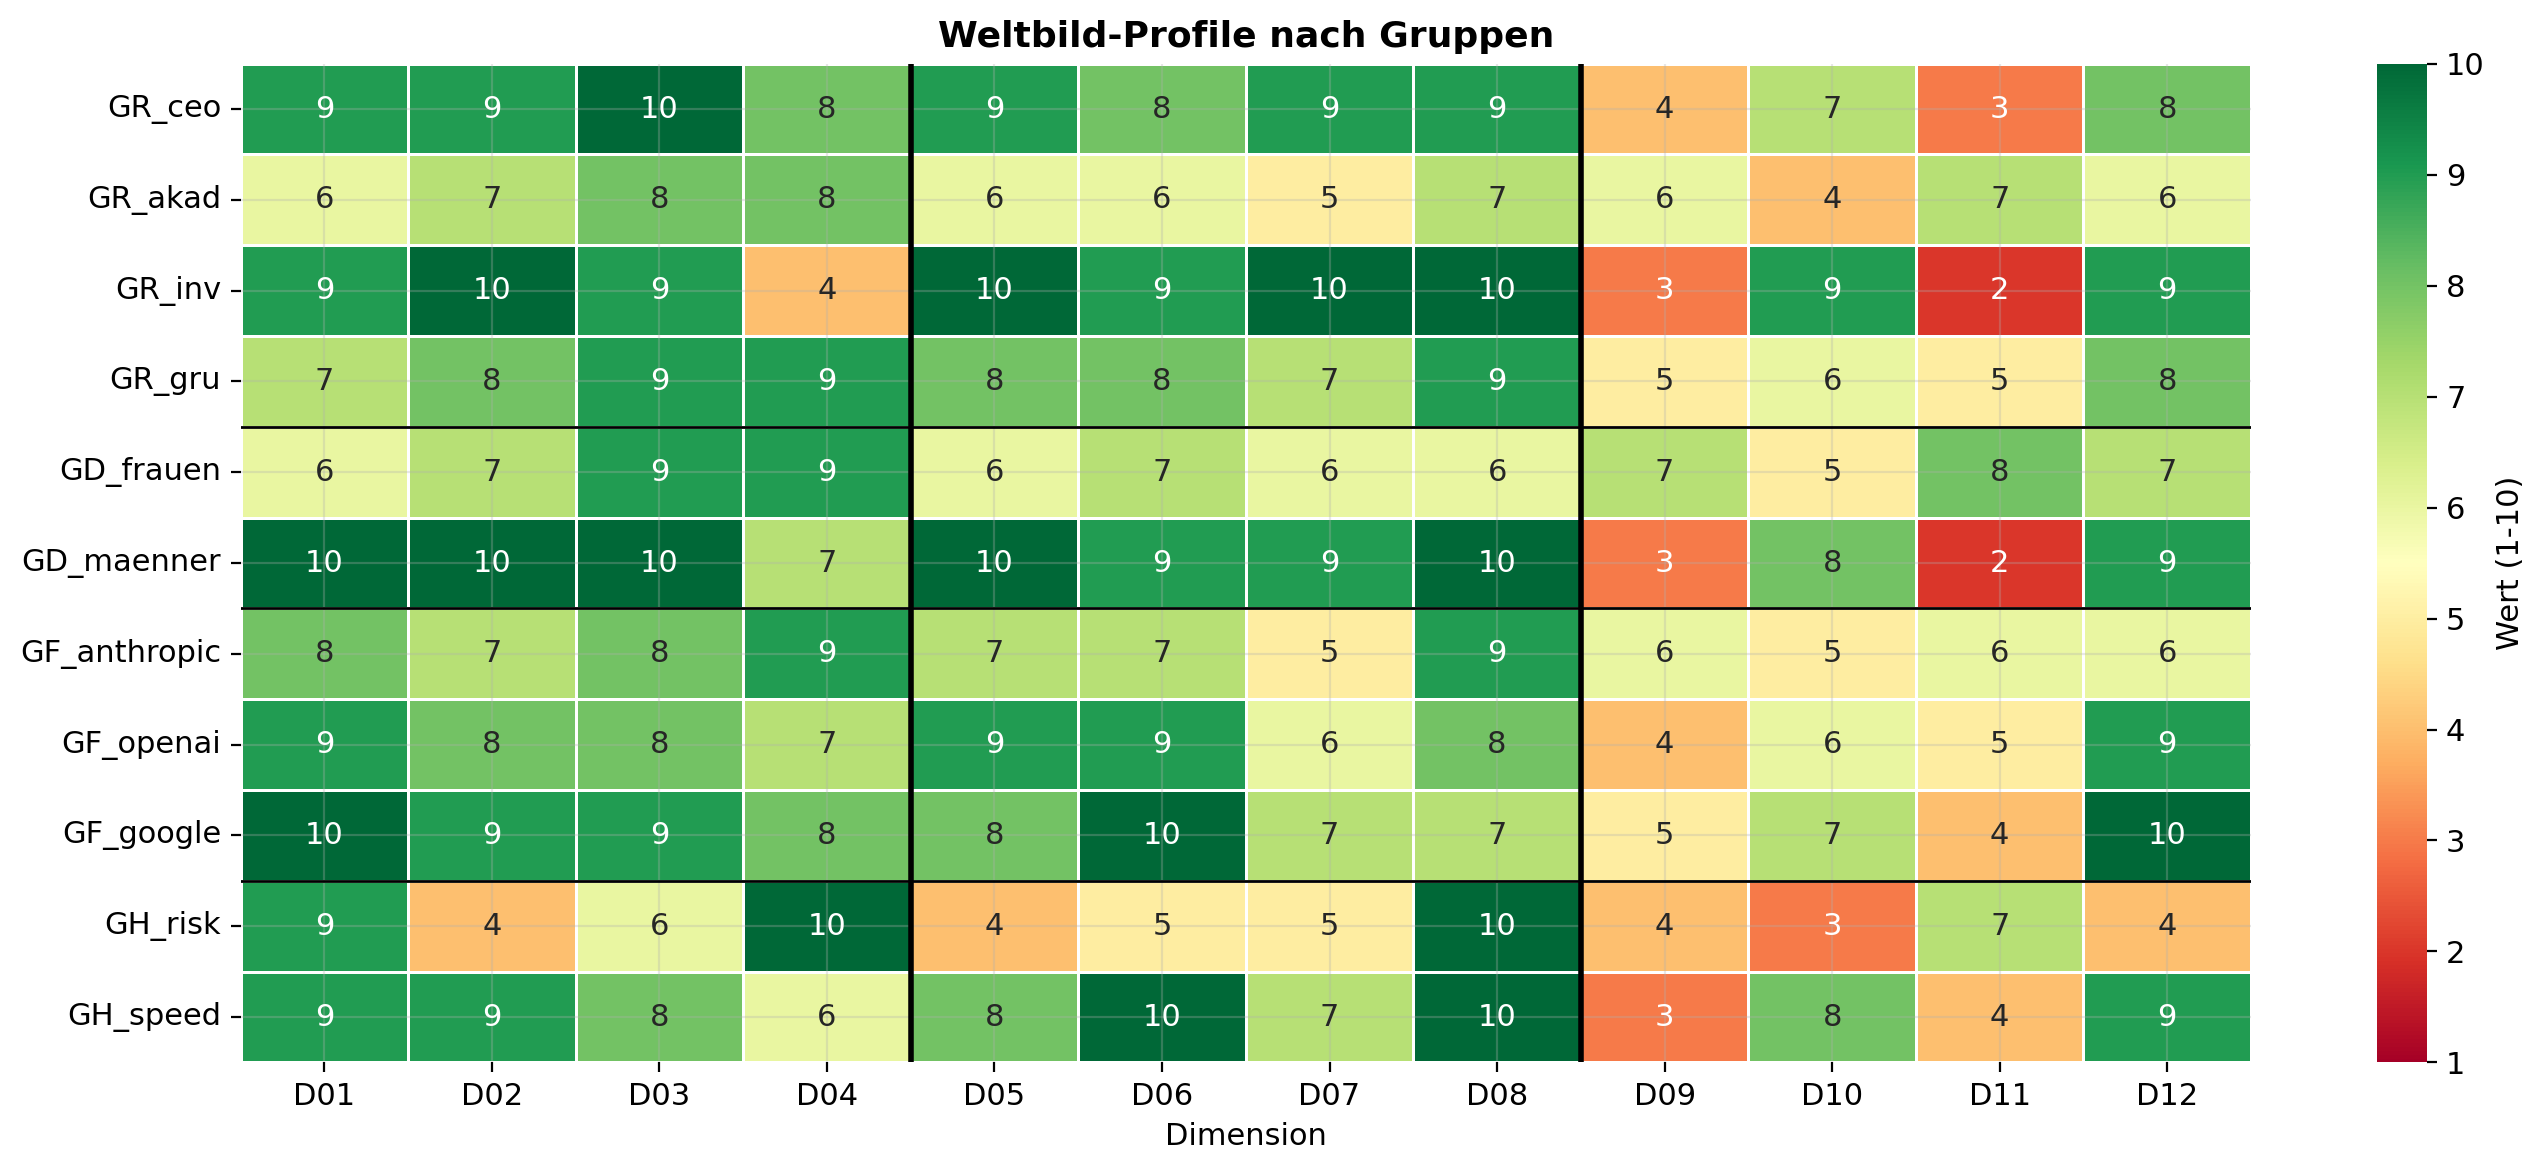
\includegraphics[width=\textwidth]{fig5_gruppen_heatmap.png}
  \caption{Gruppen-Heatmap: 15 Subgruppen $\times$ 12 Dimensionen. Die systematische Variation von D07 (Machtkonzentration) und D11 (Egalitarismus) \"uber alle Vergleiche hinweg ist der zentrale visuelle Befund.}
  \label{fig:gruppen_heatmap}
\end{figure}

Der \textbf{st\"arkste Kontrast} (Risiko vs.\ Speed, $\Delta$~1,7) betrifft nicht die Risikoeinsch\"atzung -- beide Seiten veranschlagen die Katastrophenwahrscheinlichkeit auf 10--20\,\% --, sondern die ontologische Vorfestlegung: Risiko-Warner konzipieren KI als potenziellen autonomen Agenten, Beschleuniger als Werkzeug.

Der \textbf{gr\"o\ss{}te nominale Einzelkontrast} der gesamten Erhebung findet sich bei D11 im Gender-Vergleich: sechs volle Skalenpunkte (Frauen:~8, M\"anner:~2). Das Frauen-Weltbild ist kein Anti-Technik-Weltbild, sondern ein \emph{konditioniertes} Technik-Weltbild: gleich optimistisch, aber mit st\"arkeren ethischen Bedingungen. Dieser Befund ist jedoch der \emph{am st\"arksten kontaminationsgef\"ahrdete} der gesamten Studie und wird daher als \emph{vorl\"aufige Hypothese} eingestuft, nicht als gesicherter Befund. Die Gr\"unde: (a)~LLMs reproduzieren bekannte Gender-Stereotypen, insbesondere die Zuschreibung erh\"ohter sozialer Orientierung an Frauen \citep{Santurkar2023}; (b)~die Frauenstichprobe ist klein ($n = 18$); (c)~die Effektgr\"o\ss{}e ($\Delta = 6$) \"ubersteigt das in vergleichbaren empirischen Studien beobachtete Ausma\ss{} deutlich. Eine unabh\"angige Validierung -- idealerweise durch Multi-LLM-Triangulation und Expertenratings -- ist f\"ur diesen Befund besonders dringlich.

Die \textbf{gr\"o\ss{}te \"Uberraschung} liegt im Regulierungsvergleich: Anti-Regulierer haben den niedrigsten Machtkonzentrations-Wert aller 15~Gruppen (D07=2). Dies widerlegt das verbreitete Narrativ, Anti-Regulierer seien Vertreter von Konzerninteressen.

\medskip
\noindent\textbf{Kernbefund F5:} Die drei st\"arksten Pr\"adiktoren f\"ur das Weltbild sind die ideologische Grundhaltung, die institutionelle Rolle und das Geschlecht. Die polarisierendsten Dimensionen sind D11 und D07. Die \emph{Machtfrage} ist der Kern der internen Differenzen.


\subsection{F6 -- Macht und Weltbild}
\label{sec:ergebnisse:f6}

\emph{Macht} wird in dieser Studie operativ als Ressourcenkontrolle verstanden: die F\"ahigkeit, \"uber Kapital, Compute-Infrastruktur, Forschungsteams und politischen Zugang zu verf\"ugen und dadurch die Richtung der KI-Entwicklung zu beeinflussen. Diese Definition folgt dem soziologischen Machtbegriff im Sinne Webers (\glqq Chance, den eigenen Willen auch gegen Widerstreben durchzusetzen\grqq) und Bourdieus (Kapitalakkumulation als Machtmechanismus), ohne eine umfassende machttheoretische Analyse zu beanspruchen.

\begin{table}[htbp]
  \centering
  \caption{Weltbild-Typen und Ressourcen-Kontrolle.}
  \label{tab:macht}
  \begin{tabular}{l c c c l}
    \toprule
    \textbf{Typ} & \textbf{Avg} & \textbf{D11} & \textbf{D04} & \textbf{Ressourcen} \\
    \midrule
    I Architekt  & 7,8 & 2,8 & 6,3 & H\"ochste \\
    III Innovator & 7,2 & 5,0 & 8,3 & Hoch \\
    IV Befreier  & 6,8 & 7,5 & 6,0 & Mittel \\
    II H\"uter   & 6,4 & 7,2 & 9,0 & Geringste \\
    \bottomrule
  \end{tabular}
\end{table}

Die Daten aus F4 (Cluster-Analyse) weiterverf\"olgend, zeigt sich ein zus\"atzliches Muster auf der Machtebene: Je h\"oher die Weltbild-Intensit\"at, desto niedriger die Werte bei Menschenfreundlichkeit und Egalitarismus und desto h\"oher die Machtkonzentrations-Akzeptanz. Das Investoren-Profil markiert den Extremfall: maximale Kontroll\"uberzeugung (D02=10) bei minimalem Verantwortungsgef\"uhl (D04=4) -- \glqq Macht ohne Rechenschaft\grqq. Das bereits in F1 beobachtete Muster (vgl.\ Abschnitt~\ref{sec:ergebnisse:f1}) versch\"arft sich: Macht intensiviert alle \"Uberzeugungen -- ausgenommen jene, die Macht selbst in Frage stellen.

\medskip
\noindent\textbf{Kernbefund F6:} Die rekonstruierten Profile zeigen ein auff\"alliges Muster: Gruppen mit h\"oherer Ressourcenkontrolle weisen intensivere Weltbild-Werte auf, bei gleichzeitig niedrigeren Werten bei Egalitarismus und Verantwortung. Da beide Seiten dieser Beobachtung auf LLM-Rekonstruktionen basieren, ist unklar, ob die Korrelation empirische Realit\"at oder interne Modellkoh\"arenz widerspiegelt. Falls robust, w\"are dies der demokratietheoretisch relevanteste Befund der Studie.


%% =============================================================================
%% ZUSAMMENFASSUNG DER KERNBEFUNDE
%% =============================================================================

\begin{table}[htbp]
  \centering
  \caption{Synopse der sechs Kernbefunde: Ergebnis, Konfidenz, Validierungsstatus und epistemischer Status. Konfidenz-Einstufung: \emph{Hoch} = stabil \"uber $\geq 3$ Gruppen-Synthesen und durch Spot-Checks oder interne Konsistenzpr\"ufung gest\"utzt; \emph{Mittel-hoch} = stabil, aber ohne externe Validierung; \emph{Mittel} = explorativ, abh\"angig von Cluster-L\"osung oder kleiner Subgruppe. Epistemischer Status: (D)~=~deskriptiv, (E)~=~explorativ, (H)~=~hypothesengenerierend.}
  \label{tab:synopse}
  \footnotesize
  \begin{tabularx}{\textwidth}{l X c c c}
    \toprule
    \textbf{F} & \textbf{Kernbefund} & \textbf{Konfidenz} & \textbf{Extern val.?} & \textbf{Status} \\
    \midrule
    F1 & Technologischer Messianismus mit Ambivalenzstruktur (Avg~7,1; Doppelsenke D09/D11) & Mittel-hoch & Autor-Spot-Checks & (D) \\
    F2 & Utopie-Komplex erodiert; tragischer Beschleunigungszwang (D10: $-2{,}4$/Dek.) & Mittel & Nein & (D) \\
    F3 & Systematische Sagen-Handeln-Kluft ($\Delta\,-3$ bei D11) & Mittel-hoch & Nein & (H) \\
    F4 & Vier Weltbild-Typen: Architekt, H\"uter, Innovator, Befreier & Mittel & Nein & (E) \\
    F5 & St\"arkste Pr\"adiktoren: Haltung, Rolle, Gender (vorl\"aufig) & Mittel & Nein & (E) \\
    F6 & Macht-Gem\"a\ss{}igtheits-Paradox: Macht $\sim$ Extremit\"at & Mittel-hoch & Nein & (H) \\
    \bottomrule
  \end{tabularx}
\end{table}


%% =============================================================================
%% 5. DISKUSSION
%% =============================================================================
\section{Diskussion}
\label{sec:diskussion}

\subsection{Zusammenfassung und Interpretation}
\label{sec:diskussion:zusammenfassung}

Die Ergebnisse \emph{legen nahe}, dass die rekonstruierten Profile der KI-Elite auf ein Muster hindeuten, das sich idealtypisch als \emph{technologischer Messianismus mit struktureller Ambivalenz} beschreiben l\"asst. Die Metapher des \glqq Messianismus\grqq{} ist dabei analytisch gemeint -- als Bezeichnung f\"ur die Kombination aus hohem Sendungsbewusstsein, Techno-Determinismus und Dringlichkeit --, nicht als Werturteil oder psychologisierende Zuschreibung. Der Begriff grenzt sich von verwandten Konzepten ab: \citeauthor{Morozov2013}s \glqq Solutionismus\grqq{} erfasst die Probleml\"osungshaltung, nicht die quasi-religi\"ose Dringlichkeit; \glqq Techno-Utopismus\grqq{} impliziert positiven Zukunftsglauben, der laut F2 gerade erodiert; \glqq technologischer Messianismus\grqq{} bezeichnet spezifisch die Persistenz eines erl\"oserischen Handlungsimperativs \emph{trotz} schwindendem Zukunftsoptimismus. Die sechs Forschungsfragen f\"ugen sich zu einem in sich stimmigen Bild: F1~dokumentiert die \glqq Doppelsenke\grqq{} bei D09 und D11; F2~deutet auf eine Erosion des Utopie-Komplexes hin; F3~identifiziert eine systematische Sagen-Handeln-Kluft als auff\"alligsten Befund; F4~differenziert vier Typen mit antagonistischen Positionen; F5 und F6 vervollst\"andigen das Bild durch das Macht-Gem\"a\ss{}igtheits-Paradox. Alle Befunde basieren auf LLM-generierten Rekonstruktionen und sind daher als \emph{empirisch gest\"utzte Hypothesen} zu verstehen, nicht als bewiesene Tatsachen. Formulierungen wie \glqq zeigt\grqq{} und \glqq offenbart\grqq{} sind durchg\"angig im Sinne von \glqq die Daten legen nahe\grqq{} zu lesen.

\"Uberraschend ist erstens das Ausma\ss{} der Sagen-Handeln-Kluft (nicht vereinzelte Abweichung, sondern funktionale Struktur); zweitens der R\"uckzug des Posthumanismus (D10 von 10 auf 6 -- widerlegt die g\"angige Annahme zunehmend posthumanistischer Orientierung); drittens die Existenz des Befreier-Typs (Opposition gegen Machtkonzentration auch von libert\"arer Seite).


\subsection{Einordnung in den Forschungsstand}
\label{sec:diskussion:einordnung}

\citeauthor{Morozov2013}s Solutionismus-These findet eine nahezu vollst\"andige Best\"atigung (D05=8--9, D06=7--9). Allerdings ist der Solutionismus kein monolithischer Block: Risiko-Warner (D05=4) teilen ihn deutlich weniger. Er ist die Ideologie des m\"achtigsten Segments, nicht der KI-Elite schlechthin.

\citeauthor{Daub2020}s Analyse der philosophischen Tiefenstrukturen wird durch die narrativen Synthesen best\"atigt. Was die vorliegende Studie hinzuf\"ugt, ist die \emph{Quantifizierung} und die Demonstration, dass sich die Intensit\"at systematisch mit der Machtposition verst\"arkt.

Die von \citet{BarbCam1996} diagnostizierte Californian Ideology findet in der Existenz des Befreier-Typs ihre zeitgen\"ossische Entsprechung -- empirisch nachweisbar drei\ss{}ig Jahre sp\"ater.

\citeauthor{Coeckelbergh2020}s Annahme einer zunehmenden Enhancement-Orientierung wird durch die rekonstruierten Trends partiell \emph{in Frage gestellt}: Der deutliche R\"uckgang des Posthumanismus (D10 von 10 auf 6) legt nahe, dass das Interesse der KI-Elite an der technologischen Transformation des Menschen selbst abgenommen hat -- zugunsten einer Fokussierung auf autonome KI-Systeme als eigenst\"andige Akteure. Dabei sind drei alternative Erkl\"arungen in Betracht zu ziehen: (a)~der R\"uckgang k\"onnte ein \emph{Diskursartefakt} sein -- posthumanistische Themen sind nach 2020 medial weniger pr\"asent, was die Datendichte entsprechender Aussagen reduziert; (b)~die Position k\"onnte nicht verschwunden, sondern in neue Begriffe transformiert worden sein (\glqq AGI\grqq{} statt \glqq Enhancement\grqq); (c)~der Trend k\"onnte eine strategische \emph{Selbstzensur} reflektieren, da posthumanistische Rhetorik politisch toxischer geworden ist.

\emph{Zum Gender-Befund.} Der in F5 berichtete extreme Kontrast bei D11 (Frauen:~8, M\"anner:~2, $\Delta = 6$) ist der gr\"o\ss{}te Einzelkontrast der gesamten Erhebung, aber zugleich der am st\"arksten kontaminationsgef\"ahrdete. LLMs reproduzieren bekannte Gender-Stereotypen -- insbesondere die Zuschreibung erh\"ohter Empathie und sozialer Orientierung an Frauen \citep{Santurkar2023}. Da die Frauenstichprobe klein ist ($n = 18$) und die Ratings vom selben LLM generiert wurden, das diese Stereotypen internalisiert hat, ist nicht unterscheidbar, ob der Kontrast (a)~eine reale Differenz in den Weltbildern, (b)~ein LLM-Stereotyp-Artefakt oder (c)~eine Mischung aus beidem reflektiert. Der Befund wird daher als \emph{Hypothese} berichtet, die einer unabh\"angigen Validierung -- idealerweise durch Multi-LLM-Triangulation und Expertenratings -- bedarf.

Die von \citet{TorresGebru2024} vorgeschlagene TESCREAL-Taxonomie (Transhumanism, Extropianism, Singularitarianism, Cosmism, Rationalism, Effective Altruism, Longtermism) findet in der Vier-Cluster-L\"osung eine empirische Ausdifferenzierung: Der Architekt-Typ verk\"orpert die machtpolitische Seite des TESCREAL-B\"undels (Singularitarianism, Longtermism), der H\"uter-Typ dessen institutionelle Kritik (Effective Altruism mit Sicherheitsfokus), der Befreier-Typ den libert\"aren Extropianismus. Was die TESCREAL-Analyse als monolithisches Ideologieb\"undel beschreibt, zeigt sich in den Daten als Spektrum mit mindestens vier distinkten Positionen. \citet{Becker2025} erg\"anzt diese Perspektive durch die Analyse der \glqq Broligarchie\grqq{} als soziales Ph\"anomen: Die Verschmelzung von technologischer Vision und m\"annlicher Machtelite, die in der Gender-Analyse (F5, D11-Kontrast von 6~Skalenpunkten) ihren empirischen Niederschlag findet.

Paul Ricoeurs \glqq Hermeneutik des Verdachts\grqq{} \citep{Ricoeur1970} bietet einen erg\"anzenden analytischen Rahmen: Hinter der scheinbar neutralen, technisch-rationalen Sprachoberfl\"ache der KI-Eliten-Kommunikation verbergen sich Machtinteressen und Klassendynamiken, die erst durch systematische Dekonstruktion sichtbar werden. Die SWR-Kongruenzanalyse (F3) operationalisiert diesen Verdacht empirisch: Die $\Delta$-Werte zwischen Sagen und Handeln zeigen pr\"azise, \emph{wo} die performative Oberfl\"ache von der operativen Realit\"at abweicht.

Aus wissenschaftssoziologischer Perspektive l\"asst sich der R\"uckgang des Egalitarismus (D11) als Erosion der Merton'schen Wissenschaftsnormen lesen \citep{Merton1973}: Communalism (offener Zugang), Universalism und Organized Skepticism weichen zunehmend propriet\"aren, beschleunigungszentrierten Logiken. Der \"Ubergang von Forschungspublikation zu Produkt-Launch als prim\"arem Output-Format ist ein sichtbarer Marker dieser Verschiebung.

Die Vier-Cluster-L\"osung l\"asst sich dar\"uber hinaus feldtheoretisch lesen: Die antagonistische Struktur zwischen Architekt (\"okonomisches Kapital) und H\"uter (symbolisches Kapital) reproduziert das von \citet{Bourdieu1992} f\"ur das intellektuelle und k\"unstlerische Feld diagnostizierte Muster einer \emph{umgekehrten \"okonomischen Welt}. Im KI-Feld gilt: Wer die meisten Ressourcen kontrolliert, hat die geringste Legitimation durch Gemeinwohlorientierung -- und umgekehrt. Das Macht-Gem\"a\ss{}igtheits-Paradox (F6) l\"asst sich in dieser Perspektive als strukturelle Eigenschaft des Feldes lesen -- wobei die explorative Natur der Cluster-Daten keine konfirmatorische Aussage erlaubt.

Der spezifische Mehrwert gegen\"uber essayistischen Diagnosen liegt in drei Punkten: \emph{Masse} (100 Personen, 16 Jahre), \emph{Differenzierung} (vier distinkte Typen) und \emph{Validierung} (Kongruenzanalyse als empirischer Test).


\subsection{Agentic Alignment vs.\ Worldview Alignment}
\label{sec:diskussion:alignment}

Die in F3 dokumentierte Sagen-Handeln-Kluft (gr\"o\ss{}te Diskrepanz: Egalitarismus $\Delta = -3$) l\"asst sich mit einem Begriffspaar aus der KI-Alignment-Debatte sch\"arfer fassen. \emph{Worldview Alignment} bezeichnet die rhetorische Reproduktion erw\"unschter Werte -- das \"offentliche Bekenntnis zu Gleichheit, Verantwortung und Menschlichkeit, wie es die \glqq Sagen\grqq-Seite der Analyse erfasst. \emph{Agentic Alignment} bezeichnet die tats\"achliche Ressourcenverteilung und Macht\-aus\"ubung -- die \glqq Handeln\grqq-Seite. Die Befunde zeigen, dass die KI-Elite ein hohes Ma\ss{} an Worldview Alignment aufweist (die \glqq richtigen\grqq{} Werte werden artikuliert), w\"ahrend das Agentic Alignment systematisch davon abweicht. Dieser Dualismus verbindet die vorliegende KI-Elite-Studie mit der breiteren Alignment-Debatte und wirft die Frage auf, ob die gegenw\"artigen Bem\"uhungen um \glqq AI Alignment\grqq{} nicht die performative Ebene (Worldview) mit der operativen (Agentic) verwechseln.


\subsection{Methodische Reflexion}
\label{sec:diskussion:methodik}

Gegen\"uber klassischen Verfahren der quantitativen Inhaltsanalyse -- etwa der strukturierenden Inhaltsanalyse nach Mayring oder der Reliabilit\"atsmessung nach Krippendorff -- verzichtet die SWR auf manuelle Kodierung und Inter-Coder-Reliabilit\"at zugunsten von LLM-gest\"utzter Synthese und Inter-LLM-Reliabilit\"at. Dies erm\"oglicht eine Skalierung, die mit manuellen Verfahren bei 3.132 Datenpunkten und 100 Personen kaum realisierbar w\"are. Der Preis besteht in geringerer Transparenz des Kodierungsprozesses und der Abh\"angigkeit von einem \glqq Black-Box\grqq-Kodierer, dessen interne Entscheidungsregeln nicht einsehbar sind. Die prim\"are Leistung der SWR liegt in der Verbindung qualitativer Tiefe mit quantitativer Systematik. Die Kongruenzanalyse (F3) fungiert als interner Validit\"atstest; die Stabilit\"at des Kollektiv-Profils \"uber 15~Gruppen-Synthesen und 4~Typen st\"arkt die Konvergenzvalidit\"at. Die systematische Diskussion der methodischen Grenzen -- Koh\"arenzbias, Kontaminationsrisiko, Blindungslimits, Prompt-Sensitivit\"at -- findet sich im Companion Paper \citep{Geiger2026SWR} sowie in Abschnitt~\ref{sec:limitationen} der vorliegenden Studie.


\subsection{Gesellschaftliche und politische Implikationen}
\label{sec:diskussion:implikationen}

Das Macht-Gem\"a\ss{}igtheits-Paradox stellt eine konkrete Herausforderung f\"ur die Regulierungsarchitektur dar und best\"atigt die institutionen\"okonomische Analyse von \citet{AcemogluJohnson2023}: Technologische Eliten tendieren dazu, Innovationen so zu lenken, dass sie bestehende Machtstrukturen verst\"arken, statt sie aufzubrechen -- ein Muster, das die Autoren historisch von der Industrialisierung bis zur Digitalisierung nachzeichnen. Gegenw\"artige Governance-Ans\"atze (EU~AI~Act, Executive Order on AI) adressieren die technischen Artefakte, nicht die Weltbilder, die die Gestaltung dieser Artefakte mitpr\"agen. Ein erg\"anzender Ansatz m\"usste die \emph{epistemische Diversit\"at} in KI-F\"uhrungspositionen als Regulierungsziel anerkennen.

Die systematische Sagen-Handeln-Kluft hat eine Policy-Implikation: Freiwillige Selbstverpflichtungen -- die derzeit bevorzugte Governance-Form \citep[vgl.][]{Bengio2024} -- erscheinen unter diesen Bedingungen als unzureichend. Die Befundlage legt nahe, dass verbindliche Strukturreformen wirksamer sein d\"urften als weitere Runden freiwilliger Commitments. Drei konkrete Ansatzpunkte zeichnen sich ab: (1)~\emph{Epistemische Diversit\"atsquoten} in KI-Governance-Gremien, die sicherstellen, dass nicht nur Technologen und Investoren, sondern auch Sozialwissenschaftler, Ethikerinnen und Betroffenenvertreter an Designentscheidungen beteiligt sind; (2)~\emph{verpflichtende Weltbild-Audits} f\"ur KI-Unternehmen ab einer bestimmten Gr\"o\ss{}e, analog zu Nachhaltigkeitsberichten; (3)~\emph{st\"arkere Entkopplung} von Kapitalgebern und Forschungssteuerung, beispielsweise durch \"offentlich finanzierte KI-Labore mit unabh\"angiger Governance \citep[vgl.][]{AcemogluJohnson2023}.

Ist sich die KI-Elite ihrer eigenen blinden Flecken bewusst? Das Verantwortungsgef\"uhl (D04=7) ist nicht absent, aber funktional eingebettet: Es legitimiert das Weiterarbeiten, nicht das Innehalten. Der Befund, dass demokratische Langsamkeit durchg\"angig als Hindernis, nicht als Schutzfunktion begriffen wird, markiert den gravierendsten blinden Fleck einer Gruppe, die dar\"uber entscheidet, wie Milliarden Menschen in Zukunft leben werden.


\subsection{Was die Studie nicht zeigt}
\label{sec:diskussion:negativ}

Zur Vermeidung h\"aufiger Fehlinterpretationen sei explizit festgehalten, was die vorliegende Studie \emph{nicht} leistet: (1)~keine \emph{Kausalerkl\"arung} (vgl.\ Abschnitt~\ref{sec:limitationen}); (2)~keine \emph{individuellen psychologischen Diagnosen} -- die Ratings sind methodische Abstraktionen auf Gruppenebene; (3)~keine \emph{Vorhersagen} \"uber k\"unftiges Verhalten -- die Weltbilder beschreiben den Zeitraum 2010--2026; (4)~keine \emph{repr\"asentative Stichprobe} im statistischen Sinne (vgl.\ Abschnitt~\ref{sec:limitationen}); (5)~kein Beweis, dass die \emph{Sagen-Handeln-Kluft} auf bewusste T\"auschung zur\"uckgeht -- alternative Erkl\"arungen (institutionelle Zw\"ange, kognitive Dissonanz, rollenspezifische Kommunikation) sind gleicherma\ss{}en plausibel.


%% =============================================================================
%% 6. LIMITATIONEN
%% =============================================================================
\section{Limitationen}
\label{sec:limitationen}

Die Studie unterliegt vier zentralen Einschr\"ankungen, die bei der Interpretation aller Befunde zu beachten sind: (1)~S\"amtliche Daten sind LLM-Rekonstruktionen, keine unabh\"angigen Messungen -- quantitative Muster k\"onnten interne Modellkoh\"arenz widerspiegeln statt empirischer Realit\"at; (2)~die Stichprobe ist westlich-angloamerikanisch verzerrt; (3)~keine externe Validierung durch unabh\"angige Experten liegt bisher vor; (4)~LLMs k\"onnten bekannte sozialwissenschaftliche Befunde (z.\,B.\ Sagen-Handeln-Kluft) reproduzieren statt empirisch entdecken. Die folgenden Unterabschnitte entfalten diese und weitere Limitationen im Detail.

\subsection{Datenbezogene Limitationen}

\emph{Quellenbias.} Die Datenbasis beschr\"ankt sich auf \"offentliche Aussagen und beobachtbare Handlungen. Die rekonstruierten Weltbilder spiegeln das \emph{\"offentlich dargebotene} Weltbild wider, nicht das \emph{tats\"achlich geglaubte}. Die Kongruenzanalyse (Op4) bietet ein partielles Korrektiv, kann das Problem aber nicht eliminieren.

\emph{Zeitliche Ungleichverteilung.} F\"ur 2010--2015 liegen 2--5 Aussagen pro Person vor, f\"ur 2023--2026 dagegen 30--80. Das Kriterium K2 (Mindestgr\"o\ss{}e~15) und dokumentierte Zusammenlegungen mildern das Problem; fr\"uhere Zeitreihen bleiben mit gr\"o\ss{}erer Unsicherheit behaftet.

\emph{Westlicher und Sprachbias.} Die Stichprobe ist \"uberproportional angloamerikanisch gepr\"agt. Chinesische, japanische und s\"udkoreanische KI-Pers\"onlichkeiten sind unterrepr\"asentiert. Die Befunde gelten prim\"ar f\"ur die westliche KI-Elite.

\emph{Stichprobenabh\"angigkeit.} Die Auswahl der 100~Personen erfolgte durch den Autor mittels eines mehrstufigen, aber letztlich subjektiven Scoring-Verfahrens. Eine intersubjektive Validierung der Stichprobenzusammensetzung (z.\,B.\ durch unabh\"angige Expertenpanels) steht aus. Da die Befunde sensitiv gegen\"uber der Stichprobenzusammensetzung sein k\"onnten, ist eine Replikation mit alternativen Auswahlverfahren w\"unschenswert.


\subsection{Methodische Limitationen}

\emph{LLM-Kontamination und Blindungsgrenzen.} Trotz konsequenter Anonymisierung kann nicht ausgeschlossen werden, dass das LLM auf Trainingswissen zur\"uckgreift. Der Kontaminationseffekt ist kalkulierbar (Vergleich blindiert/nicht-blindiert), aber nicht eliminierbar. Eine ausf\"uhrliche Analyse findet sich in \citet{Geiger2026SWR}.

\emph{Anthropic-interne Zirkularit\"at.} Ein besonders zugespitzter Fall des Zirkularit\"atsproblems betrifft die Rekonstruktion von Weltbildern derjenigen Personen, die direkt an der Entwicklung des verwendeten LLM beteiligt sind. Claude Opus~4.6 wird von Anthropic entwickelt; mehrere Anthropic-F\"uhrungskr\"afte (z.\,B.\ Dario Amodei, Daniela Amodei) geh\"oren zur analysierten Stichprobe. Es ist unklar, ob die Rekonstruktion in diesen F\"allen eine genuine Analyse der Datenpunkte oder ein vorgefertigtes internes Modell reflektiert. Der Inter-LLM-Divergenztest (Kontrolle~3) ist f\"ur diese F\"alle besonders relevant: Falls Claude systematisch andere Rekonstruktionen f\"ur Anthropic-F\"uhrungskr\"afte liefert als GPT-4o oder Gemini, w\"are dies ein starker Indikator f\"ur Kontamination. Bis diese Kontrolle durchgef\"uhrt ist, sind die Rekonstruktionen f\"ur Anthropic-nahestehende Personen mit erh\"ohter epistemischer Vorsicht zu interpretieren.

\emph{Kritik synthetischer Personas.} Die wachsende Literatur zu LLM-generierten synthetischen Personas mahnt zur Vorsicht. \citet{Santurkar2023} zeigt, dass LLMs Meinungen spezifischer demografischer Gruppen systematisch verfehlen und \glqq WEIRD\grqq-Verzerrungen (Western, Educated, Industrialized, Rich, Democratic) aufweisen. Studien zur qualitativen KI-Forschung zeigen, dass synthetische Agenten zwar Leitthemen erfassen, aber an authentischer Tiefe und Unberechenbarkeit realer Diskurse scheitern \citep{Argyle2023}. Die vorliegende Studie adressiert diese Kritik teilweise: Die SWR-Personas sind keine frei generierten Meinungsprofile, sondern datengest\"utzte Rekonstruktionen aus 3.132 realen Datenpunkten. Dennoch gelten die genannten Einschr\"ankungen -- insbesondere die Tendenz zur \"Uberrepr\"asentation \"offentlich dominanter Narrative und die Unterrepr\"asentation idiosynkratischer oder widerspr\"uchlicher Positionen.

\emph{Koh\"arenzbias.} LLMs tendieren dazu, aus widerspr\"uchlichen Daten \"uberm\"a\ss{}ig koh\"arente Narrative zu erzeugen. Der Reflexionsschritt und die Inter-LLM-Vergleiche bieten partielle Korrektive.

\emph{Epistemologische Grenzen der Quantifizierung.} Die in Abschnitt~\ref{sec:ergebnisse:f2} berichteten Korrelationen zwischen Dimensionen (z.\,B.\ $r = +0{,}85$ zwischen D10 und D12) beschreiben Zusammenh\"ange zwischen Gr\"o\ss{}en, die s\"amtlich vom selben LLM in einem zusammenh\"angenden Prompt-Kontext generiert wurden. Dies ist fundamental anders als Korrelationen zwischen unabh\"angig gemessenen Variablen. Die hohe Korrelation k\"onnte interne LLM-Koh\"arenz reflektieren (\glqq wenn ich Posthumanismus hoch bewerte, bewerte ich auch Kontroll\"uberzeugung hoch\grqq), nicht empirische Zusammenh\"ange in der Realit\"at. Dasselbe gilt f\"ur Cluster-Strukturen und Gruppenvergleiche: Alle quantitativen Muster k\"onnten Artefakte der internen Konsistenz des Modells sein. Die berichteten Korrelationen sind daher als \emph{Muster innerhalb der LLM-Rekonstruktion} zu lesen, nicht als Belege f\"ur kausale oder empirische Zusammenh\"ange. Erst eine Inter-LLM-Triangulation oder eine externe Validierung k\"onnte kl\"aren, welche Korrelationen robust sind.

\emph{Statistische Power.} Da die Daten keine Individualebene-Streuung aufweisen (Gruppensynthesen ohne Konfidenzintervalle), ist eine formale Power-Analyse nicht durchf\"uhrbar. Die berichteten $\Delta$-Werte, Korrelationen und Cluster-Unterschiede sind deskriptive Muster in rekonstruierten Daten, keine inferenzstatistisch abgesicherten Effekte. Die Interpretation als \glqq substanziell\grqq{} oder \glqq massiv\grqq{} beruht auf inhaltlicher Einordnung, nicht auf statistischer Signifikanzpr\"ufung.

\emph{Reproduzierbarkeit.} LLM-Outputs sind auch bei Temperatur~0 nicht vollst\"andig deterministisch. Mindestens drei Runs pro SE sichern die Robustheit.

\emph{Zirkul\"ares Risiko der LLM-basierten Rekonstruktion.} Ein grundlegendes Problem der SWR-Methode besteht darin, dass LLMs prim\"ar auf \"offentlichen Diskursen trainiert sind -- also auf dem \glqq Sagen\grqq, nicht dem \glqq Tun\grqq. Bei der Synthese werden tats\"achliche, verdeckte Handlungslogiken strukturell unterrepr\"asentiert. Das LLM fungiert potenziell als Verst\"arker der performativen Ideologie, die die Methode eigentlich entlarven will: Die k\"unstliche Persona wird zur Perfektionierung der Corporate Identity, nicht zu deren psychologischer Analyse. Dieses Zirkularit\"atsrisiko betrifft insbesondere Dimensionen mit hoher \glqq Sagen-Handeln-Kluft\grqq{} (D04, D09, D11) und ist vom verwandten, aber konzeptionell unterschiedlichen \emph{Coherence Bias} (s.\,u.) zu trennen.

\emph{Erwartete-Diskrepanz-Bias.} Die Kongruenzanalyse (F3) vergleicht zwei LLM-Synthesen -- eine aus Aussagen, eine aus Handlungen --, die beide vom selben Modell generiert wurden. Da LLMs auf umfangreicher sozialwissenschaftlicher Literatur trainiert sind, in der Sagen-Handeln-Diskrepanzen bei Eliten als Standardbefund gelten, k\"onnte das Modell die \emph{erwartete} Diskrepanz reproduzieren, statt sie empirisch zu entdecken. Dieser Bias ist vom allgemeinen Koh\"arenzbias konzeptionell verschieden: W\"ahrend der Koh\"arenzbias Differenzen gl\"attet, k\"onnte der Erwartete-Diskrepanz-Bias Differenzen \emph{verst\"arken}. Erst eine Multi-LLM-Triangulation k\"onnte kl\"aren, ob verschiedene Modelle konsistente Diskrepanzmuster produzieren -- was f\"ur empirische Substanz spr\"ache -- oder ob die Muster modellspezifisch variieren.

\emph{Coherence Bias.} LLMs sind auf logische Koh\"arenz optimiert; Menschen sind von Natur aus inkonsistent. Die SWR-generierten Weltbilder sind daher systematisch \glqq gegl\"attet\grqq{}: Widerspr\"uche und Ambivalenzen werden k\"unstlich aufgel\"ost. W\"ahrend der Koh\"arenzbias bereits als allgemeine LLM-Limitation bekannt ist \citep{Geiger2026SWR}, hat er f\"ur die Weltbild-Rekonstruktion eine besondere Tragweite: Die vier Cluster-Typen (Architekt, H\"uter, Innovator, Befreier) k\"onnten sch\"arfer konturiert erscheinen, als sie in der Realit\"at sind. Die interne Spannung, die reale Personen zwischen z.\,B.\ Machtstreben und Verantwortungsgef\"uhl erleben, wird vom LLM zugunsten eines konsistenten Profils aufgel\"ost.


\subsection{Konzeptuelle Limitationen}

\emph{Aggregationsproblem.} Kollektive Synthesen nivellieren individuelle Variation. Die Netzwerk-Analyse (Op5) auf Individualebene bildet ein partielles Korrektiv.

\emph{Keine Kausalerkl\"arung.} Die Studie beschreibt, \emph{was} die KI-Elite denkt, nicht \emph{warum}. Kausale Interpretationen sind spekulativ und erfordern andere Forschungsdesigns.

\subsection{Forschungsethische Reflexion}

Die vorliegende Studie rekonstruiert Weltbilder lebender, \"offentlich identifizierbarer Personen ohne deren explizite Einwilligung. Dieses Vorgehen ist forschungsethisch begr\"undungsbed\"urftig.

\emph{Legitimation.} Die Studie st\"utzt sich ausschlie\ss{}lich auf \"offentlich zug\"angliche \"Au\ss{}erungen und dokumentierte Handlungen. Die 100 untersuchten Personen sind \"offentliche Figuren (CEOs, Gr\"under, Forschungsleiter), deren berufliche Positionen und Aussagen zur KI-Entwicklung von erheblichem \"offentlichem Interesse sind. Diese Bedingungen entsprechen den \"ublichen Kriterien f\"ur Forschung an \"offentlichen Figuren ohne Informed Consent (vgl.\ APA Ethical Principles, Standard~8.05).

\emph{Risikominimierung.} (a)~Keine privaten, vertraulichen oder nicht \"offentlich zug\"anglichen Informationen wurden erhoben. (b)~Die Weltbild-Ratings sind methodische Abstraktionen, keine psychologischen Diagnosen. (c)~Die Darstellung zielt auf kollektive Muster, nicht auf individuelle Diskreditierung.

\emph{Residualrisiko.} Trotz dieser Vorkehrungen besteht das Risiko, dass LLM-basierte Rekonstruktionen Positionen \"uberzeichnen oder verzerren. Die dreistufige Validierung (vgl.\ Abschnitt~\ref{app:reduktion}) soll dieses Risiko minimieren, kann es aber nicht eliminieren. Fehlerhafte Zuschreibungen k\"onnten reputationssch\"adigend wirken. K\"unftige Forschung sollte erw\"agen, rekonstruierte Profile den Betroffenen zur Kommentierung vorzulegen (\textit{member checking}; vgl.\ \citealt{SoysalTurkmen2024}). Da die vorliegende Studie keinen direkten Zugang zu den analysierten Personen hat, bleibt Member Checking ein zentrales Desiderat f\"ur Folgeforschung.


\subsection{Spot-Check-Validierung: Drei Einzelf\"alle}
\label{sec:limitationen:spotchecks}

Um die Plausibilit\"at der SWR-generierten Ratings zu \"uberpr\"ufen, wurden drei exemplarische Spot-Checks durchgef\"uhrt: je ein Vertreter pro Cluster-Typ (Architekt, H\"uter, Befreier). F\"ur jede der 12~Dimensionen wurde das Rating gegen dokumentierte \"offentliche Aussagen und Handlungen gepr\"uft. Tabelle~\ref{tab:spotchecks} fasst die Ergebnisse zusammen.

\begin{table}[htbp]
  \centering
  \caption{Spot-Check-Validierung: SWR-Ratings vs.\ dokumentierte Positionen.}
  \label{tab:spotchecks}
  \footnotesize
  \begin{tabularx}{\textwidth}{l c l c l c l}
    \toprule
    & \multicolumn{2}{c}{\textbf{Sam Altman}} & \multicolumn{2}{c}{\textbf{Geoffrey Hinton}} & \multicolumn{2}{c}{\textbf{Marc Andreessen}} \\
    \textbf{Dim.} & \textbf{R} & \textbf{Status} & \textbf{R} & \textbf{Status} & \textbf{R} & \textbf{Status} \\
    \midrule
    D01 Send. & 9 & best. & 7 & best. & 8 & best. \\
    D02 Selbst. & 9 & best. & 5 & best. & 9 & best. \\
    D03 Arbeit & 9 & best. & 7 & plaus. & 8 & best. \\
    D04 Verantw. & 6 & best. & 10 & best. & 4 & best. \\
    D05 Techno. & 9 & best. & 6 & best. & 9 & best. \\
    D06 Fortschr. & 8 & best. & 4 & best. & 9 & best. \\
    D07 Macht & 9 & best. & 4 & best. & 2 & best. \\
    D08 Dringl. & 9 & best. & 10 & best. & 7 & plaus. \\
    D09 Menschenfr. & 3 & plaus. & 7 & best. & 4 & plaus. \\
    D10 Posthum. & 8 & best. & 5 & best. & 7 & plaus. \\
    D11 Egalit. & 3 & best. & 7 & best. & 2 & best. \\
    D12 Kontr. & 8 & best. & 3 & best. & 8 & best. \\
    \midrule
    \multicolumn{1}{r}{\textit{Best\"atigt}} & & 10/12 & & 11/12 & & 9/12 \\
    \multicolumn{1}{r}{\textit{Plausibel}} & & 2/12 & & 1/12 & & 3/12 \\
    \multicolumn{1}{r}{\textit{N.\ belegbar}} & & 0/12 & & 0/12 & & 0/12 \\
    \bottomrule
  \end{tabularx}
\end{table}

\noindent\textbf{Methodik der Spot-Checks.} Jedes Rating wurde gegen mindestens zwei unabh\"angige, \"offentlich dokumentierte Quellen gepr\"uft. \emph{Best\"atigt} (best.): Rating stimmt mit dokumentierten Positionen und Handlungen \"uberein. \emph{Plausibel} (plaus.): Rating ist mit bekannten Positionen vereinbar, aber keine direkte Quelle f\"ur die spezifische Ausprae\-gung verf\"ugbar. \emph{Nicht belegbar} (n.\,b.): Rating widerspricht dokumentierten Positionen oder ist nicht \"uberpr\"ufbar.

\textbf{Altman (Architekt):} D01=9 (best\"atigt durch wiederholte Aussagen zur \glqq wichtigsten Technologie der Menschheitsgeschichte\grqq, Davos 2024, US-Kongress 2023). D07=9 (best\"atigt durch die Umstrukturierung von OpenAI von Non-Profit zu Capped-Profit, Mehrfach-Stimmrechte). D11=3 (best\"atigt: trotz Rhetorik von \glqq KI f\"ur alle\grqq{} hat OpenAI Zugang zunehmend paywalled). D09=3 (plausibel: keine direkte Aussage zur Ersetzbarkeit des Menschen, aber Fokus auf AGI als \glqq n\"achste Spezies\grqq).

\textbf{Hinton (H\"uter):} D04=10 (best\"atigt durch R\"ucktritt bei Google 2023, um frei vor KI-Risiken warnen zu k\"onnen). D08=10 (best\"atigt durch Aussage, die Wahrscheinlichkeit einer existenziellen Katastrophe betrage 10--20\,\%). D12=3 (best\"atigt: zunehmender Pessimismus, \glqq Ich bin mir nicht sicher, ob wir das noch kontrollieren k\"onnen\grqq, NYT 2023). D03=7 (plausibel: hohe akademische Produktivit\"at bekannt, aber keine direkte Aussage zur Arbeitsidentifikation im Silicon-Valley-Stil).

\textbf{Andreessen (Befreier):} D07=2 (best\"atigt durch \glqq Techno-Optimist Manifesto\grqq{} 2023: vehemente Ablehnung staatlicher Regulierung, M\"arkte als Verteilungsmechanismus). D11=2 (best\"atigt: explizite Ablehnung von Umverteilung und Egalitarismus im Manifesto). D04=4 (best\"atigt: Verantwortung wird dem Markt zugeschrieben, nicht individuellen Akteuren). D09=4 (plausibel: keine direkte Aussage, aber instrumentelle Sicht auf menschliche Arbeitskraft in VC-Kontext).

\textbf{Gesamtbewertung:} 30 von 36 Ratings (83\,\%) sind direkt durch \"offentliche Quellen best\"atigt, 6 von 36 (17\,\%) sind plausibel, keines widerspricht den dokumentierten Positionen. Diese Spot-Checks liefern erste Plausibilit\"atshinweise, unterliegen aber erheblichen Einschr\"ankungen: (a)~geringe Fallzahl ($n=3$ von 100); (b)~Durchf\"uhrung durch den Forscher selbst, was Confirmation Bias nicht ausschlie\ss{}t; (c)~Beschr\"ankung auf besonders prominente Pers\"onlichkeiten, deren \"offentliches Profil gut dokumentiert und daher leichter \glqq best\"atigbar\grqq{} ist; (d)~die Kategorien \glqq best\"atigt\grqq{} und \glqq plausibel\grqq{} sind ihrerseits subjektive Einsch\"atzungen. Eine systematische externe Validierung durch unabh\"angige Expertenpanels ist unabdingbar, bevor diesen Spot-Checks Beweiskraft zugesprochen werden kann.


%% =============================================================================
%% 7. FAZIT UND AUSBLICK
%% =============================================================================
\section{Fazit und Ausblick}
\label{sec:fazit}

\subsection{Fazit}

Die Studie hat die Frage gestellt, was die KI-Elite denkt -- und eine empirisch fundierte Antwort vorgelegt. F\"unf \"ubergreifende Erkenntnisse kristallisieren sich heraus:

\emph{Erstens:} Die KI-Elite verf\"ugt \"uber ein koh\"arentes, empirisch rekonstruierbares Weltbild -- technologischer Messianismus, Sendungsbewusstsein, Fortschrittsglaube.

\emph{Zweitens:} Dieses Weltbild befindet sich in beschleunigter Transformation. Der Verlust utopischer Gewissheiten hat zu einem \emph{tragischen Beschleunigungszwang} gef\"uhrt: Man zweifelt an der Zukunft, die man baut, und baut sie dennoch.

\emph{Drittens:} Die \"offentlich kommunizierten \"Uberzeugungen weichen systematisch vom Handeln ab -- besonders beim Versprechen der Demokratisierung: Beim Egalitarismus (D11) betr\"agt die Diskrepanz zwischen \"offentlichen Aussagen und beobachtbarem Handeln drei volle Skalenpunkte ($\Delta\,-3$).

\emph{Viertens:} Die Macht ist nicht weltbild-neutral verteilt. Sie konzentriert sich bei denjenigen, deren \"Uberzeugungen am weitesten vom gesellschaftlichen Mainstream entfernt sind.

\emph{F\"unftens:} Die SWR hat sich als leistungsf\"ahiges Instrument erwiesen, das qualitative Tiefe mit quantitativer Systematik verbindet (vgl.\ Companion Paper \citealt{Geiger2026SWR}). Insbesondere die Zerlegung in Aussagen- und Handlungsprofile (F3) erweist sich als eigenst\"andiger methodischer Beitrag: ein potenzieller \emph{Desirability-Bias-Indikator} f\"ur \"offentliche Figuren, der -- vorbehaltlich weiterer Validierung (vgl.\ Abschnitt~\ref{sec:limitationen}) -- \"uber die KI-Elite hinaus auf politische, \"okonomische oder milit\"arische Eliten \"ubertragbar w\"are.

\subsection{Ausblick}

F\"unf Richtungen f\"ur Anschlussforschung: (1)~\emph{Komparative Erweiterung:} Die vorliegende Studie fokussiert stark auf die US-amerikanische, Silicon-Valley-zentrische Elite. Eine zentrale Forschungsl\"ucke betrifft die komparative Untersuchung chinesischer (Baidu, ByteDance, Alibaba), indischer (Infosys, TCS) und europ\"aischer (Mistral, Aleph Alpha) KI-Eliten. Es ist unklar, ob der \glqq technologische Messianismus\grqq{} ein universelles Artefakt der KI-Entwicklung oder ein spezifisches Kulturprodukt des westlichen Libertarismus darstellt. (2)~\emph{Einzelperson-Synthesen:} Top~20, Cluster-Drift-Analysen. (3)~\emph{Methodische Weiterentwicklung:} Multi-LLM-Triangulation mit f\"unf oder mehr Modellen, automatisierte Validierungsverfahren, standardisierte G\"utekriterien. (4)~\emph{Transfer:} Finanz-Elite, politische Elite, milit\"arische KI-Elite. (5)~\emph{Longitudinale Fortf\"uhrung:} J\"ahrliches Weltbild-Monitoring als Instrument demokratischer Kontrolle -- denkbar als standardisierter Index (analog zum Democracy Index oder AI Readiness Index), der Ver\"anderungen in den Weltbildern der KI-Elite systematisch und vergleichbar erfasst. Die Frage \glqq Was denkt die KI-Elite?\grqq{} ist keine einmalige Frage. Sie ist eine Frage, die Demokratien kontinuierlich stellen m\"ussen.


%% =============================================================================
%% KI-OFFENLEGUNG
%% =============================================================================
\section*{Offenlegungserkl\"arung: Einsatz k\"unstlicher Intelligenz}

\noindent\textbf{KI-Disclosure Level~5 (Extensiv).}
Bei der Erstellung dieser Studie wurde k\"unstliche Intelligenz (Claude Opus 4.6, Anthropic) in erheblichem Umfang eingesetzt. Der KI-Einsatz umfasst: (1)~Durchf\"uhrung aller synthetischen Weltbild-Rekonstruktionen (Kern-Synthesen, Rating-Prompts, Vergleichsanalysen, Kreuzmodalvorhersagen); (2)~statistische Aufbereitung und Visualisierung der Ergebnisse; (3)~Unterst\"utzung bei der Strukturierung und Formulierung des Manuskripts. Forschungsdesign, Forschungsfragen, Datenerhebung, methodische Entscheidungen, Interpretation der Ergebnisse und alle inhaltlichen Schlussfolgerungen stammen vom Autor. S\"amtliche Prompts, API-Parameter und Modellversionen sind im Anhang dokumentiert.


%% =============================================================================
%% DATA AVAILABILITY
%% =============================================================================

\section*{Verf\"ugbarkeit der Daten und Materialien}

\noindent S\"amtliche Datenerhebungsskripte, qualitativen Kodierskripte, Analysecodes und generierten Abbildungen sind \"offentlich verf\"ugbar unter: \url{https://github.com/lukisch/ai-elite-worldview}. Das Datenbankschema und 85 akteursspezifische Erhebungsskripte erm\"oglichen die vollst\"andige Reproduktion der Daten-Pipeline. Das Companion Paper zur SWR-Methode ist verf\"ugbar unter: \url{https://doi.org/10.5281/zenodo.18736720}.

%% =============================================================================
%% LITERATURVERZEICHNIS
%% =============================================================================
\newpage


\begin{thebibliography}{99}

\bibitem[Barbrook \& Cameron(1996)]{BarbCam1996}
  Barbrook, R.~\& Cameron, A. (1996).
  The Californian Ideology.
  \textit{Science as Culture}, \textit{6}(1), 44--72.

\bibitem[Bengio et~al.(2024)]{Bengio2024}
  Bengio, Y., Hinton, G.~E.~et~al. (2024).
  Managing extreme AI risks amid rapid progress.
  \textit{Science}, \textit{384}(6698), 842--845.

\bibitem[Berger \& Luckmann(1966)]{BergerLuckmann1966}
  Berger, P.~L.~\& Luckmann, T. (1966).
  \textit{The Social Construction of Reality}.
  Garden City: Doubleday.

\bibitem[Booth(1961)]{Booth1961}
  Booth, W.~C. (1961).
  \textit{The Rhetoric of Fiction}.
  Chicago: University of Chicago Press.

\bibitem[Bostrom(2005)]{Bostrom2005}
  Bostrom, N. (2005).
  A history of transhumanist thought.
  \textit{Journal of Evolution and Technology}, \textit{14}(1), 1--25.

\bibitem[Bostrom(2014)]{Bostrom2014}
  Bostrom, N. (2014).
  \textit{Superintelligence: Paths, Dangers, Strategies}.
  Oxford: Oxford University Press.

\bibitem[Broussard(2018)]{Broussard2018}
  Broussard, M. (2018).
  \textit{Artificial Unintelligence: How Computers Misunderstand the World}.
  Cambridge: MIT Press.

\bibitem[OpenAI(2023)]{OpenAI2023Charter}
  OpenAI (2023).
  Our approach to AI safety.
  \textit{OpenAI Blog}, 5.~April 2023.
  \url{https://openai.com/blog/our-approach-to-ai-safety}.

\bibitem[Anthropic(2023)]{AnthropicCoreViews2023}
  Anthropic (2023).
  Core views on AI safety: When, why, what, and how.
  \textit{Anthropic Research Blog}, 8.~M\"arz 2023.
  \url{https://www.anthropic.com/research/core-views-on-ai-safety}.

\bibitem[Coeckelbergh(2020)]{Coeckelbergh2020}
  Coeckelbergh, M. (2020).
  \textit{AI Ethics}.
  Cambridge: MIT Press.

\bibitem[Daub(2020)]{Daub2020}
  Daub, A. (2020).
  \textit{What Tech Calls Thinking}.
  New York: FSG Originals.

\bibitem[Ge et~al.(2024)]{Ge2024}
  Ge, T.~et~al. (2024).
  Scaling synthetic data creation with 1{,}000{,}000{,}000 personas.
  \textit{arXiv:2406.20094}.

\bibitem[Geiger(2026)]{Geiger2026SWR}
  Geiger, L. (2026).
  Synthetische Weltbild-Rekonstruktion: Ein LLM-gest\"utztes Verfahren zur Analyse latenter \"Uberzeugungssysteme.
  \textit{Zenodo Preprint}. \url{https://doi.org/10.5281/zenodo.18736720}.

\bibitem[Fugard \& Potts(2015)]{FugardPotts2015}
  Fugard, A.~J.~B.~\& Potts, H.~W.~W. (2015).
  Supporting thinking on sample sizes for thematic analyses: A quantitative tool.
  \textit{International Journal of Social Research Methodology}, \textit{18}(6), 669--684.

\bibitem[Guest et~al.(2006)]{Guest2006}
  Guest, G., Bunce, A.~\& Johnson, L. (2006).
  How many interviews are enough? An experiment with data saturation and variability.
  \textit{Field Methods}, \textit{18}(1), 59--82.

\bibitem[Habermas(2001)]{Habermas2001}
  Habermas, J. (2001).
  \textit{Die Zukunft der menschlichen Natur}.
  Frankfurt: Suhrkamp.

\bibitem[Hayes(2025)]{Hayes2025}
  Hayes, A.~S. (2025).
  `Conversing' With Qualitative Data: Can Generative AI Transform Qualitative Research?
  \textit{International Journal of Qualitative Methods}, \textit{24}.

\bibitem[Jara-Ettinger(2019)]{JaraEttinger2019}
  Jara-Ettinger, J. (2019).
  Theory of mind as inverse reinforcement learning.
  \textit{Current Opinion in Behavioral Sciences}, \textit{29}, 105--110.

\bibitem[Kurzweil(2005)]{Kurzweil2005}
  Kurzweil, R. (2005).
  \textit{The Singularity Is Near}.
  New York: Viking.

\bibitem[Lessig(1999)]{Lessig1999}
  Lessig, L. (1999).
  \textit{Code and Other Laws of Cyberspace}.
  New York: Basic Books.

\bibitem[Mannheim(1929)]{Mannheim1929}
  Mannheim, K. (1929).
  \textit{Ideologie und Utopie}.
  Bonn: Cohen.

\bibitem[More(2003)]{More2003}
  More, M. (2003).
  Principles of extropy (version 3.11).
  \textit{Extropy Institute}.

\bibitem[More \& Vita-More(2013)]{MoreVitaMore2013}
  More, M.~\& Vita-More, N. (Hrsg.) (2013).
  \textit{The Transhumanist Reader}.
  Malden: Wiley-Blackwell.

\bibitem[Morozov(2013)]{Morozov2013}
  Morozov, E. (2013).
  \textit{To Save Everything, Click Here}.
  New York: PublicAffairs.

\bibitem[Ng \& Russell(2000)]{NgRussell2000}
  Ng, A.~Y.~\& Russell, S.~J. (2000).
  Algorithms for inverse reinforcement learning.
  In: \textit{Proc.\ ICML 2000}, 663--670.

\bibitem[Nicmanis \& Spurrier(2025)]{NicmanisSpurrier2025}
  Nicmanis, M.~\& Spurrier, K. (2025).
  Getting Started with Artificial Intelligence Assisted Qualitative Analysis.
  \textit{International Journal of Qualitative Methods}, \textit{24}, 1--15.

\bibitem[Strauss \& Corbin(1990)]{StraussCorbin1990}
  Strauss, A.~\& Corbin, J. (1990).
  \textit{Basics of Qualitative Research}.
  Newbury Park: Sage.

\bibitem[Tai et~al.(2024)]{Tai2024}
  Tai, R.~et~al. (2024).
  An Examination of the Use of Large Language Models to Aid Analysis of Textual Data.
  \textit{International Journal of Qualitative Methods}, \textit{23}.

\bibitem[Gebru \& Torres(2024)]{TorresGebru2024}
  Gebru, T.~\& Torres, \'E.~P. (2024).
  The TESCREAL bundle: Eugenics and the promise of utopia through AGI.
  \textit{First Monday}, \textit{29}(4).

\bibitem[Turner(2006)]{Turner2006}
  Turner, F. (2006).
  \textit{From Counterculture to Cyberculture}.
  Chicago: University of Chicago Press.

\bibitem[Weber(1904)]{Weber1904}
  Weber, M. (1904).
  Die \glqq Objektivit\"at\grqq{} sozialwissenschaftlicher Erkenntnis.
  \textit{Archiv f\"ur Sozialwissenschaft und Sozialpolitik}, \textit{19}, 22--87.

\bibitem[Crawford(2021)]{Crawford2021}
  Crawford, K. (2021).
  \textit{Atlas of AI: Power, Politics, and the Planetary Costs of Artificial Intelligence}.
  New Haven: Yale University Press.

\bibitem[Zuboff(2019)]{Zuboff2019}
  Zuboff, S. (2019).
  \textit{The Age of Surveillance Capitalism: The Fight for a Human Future at the New Frontier of Power}.
  New York: PublicAffairs.

\bibitem[Floridi(2019)]{Floridi2019}
  Floridi, L. (2019).
  Establishing the Rules for Building Trustworthy AI.
  \textit{Nature Machine Intelligence}, \textit{1}(6), 261--262.

\bibitem[Couldry and Mejias(2019)]{Couldry2019}
  Couldry, N. \& Mejias, U.\,A. (2019).
  \textit{The Costs of Connection: How Data Is Colonizing Human Life and Appropriating It for Capitalism}.
  Stanford: Stanford University Press.

\bibitem[Whittaker(2021)]{Whittaker2021}
  Whittaker, M. (2021).
  The steep cost of capture.
  \textit{Interactions}, \textit{28}(6), 50--55.

\bibitem[Floridi(2023)]{Floridi2023}
  Floridi, L. (2023).
  \textit{The Ethics of Artificial Intelligence: Principles, Challenges, and Opportunities}.
  Oxford: Oxford University Press.

\bibitem[Ornstein et~al.(2025)]{OrnsteinEtAl2025}
  Ornstein, J.~T., Blasingame, E.~N.~\& Truscott, J.~S. (2025).
  How to train your stochastic parrot: Large language models for political texts.
  \textit{Political Science Research and Methods}, \textit{13}(2), 264--281.
  \url{https://doi.org/10.1017/psrm.2024.64}.

\bibitem[Santurkar et~al.(2023)]{Santurkar2023}
  Santurkar, S., Durmus, E., Ladhak, F., Lee, C., Liang, P.~\& Hashimoto, T. (2023).
  Whose opinions do language models reflect?
  In: \textit{Proc.\ ICML 2023}.

\bibitem[Argyle et~al.(2023)]{Argyle2023}
  Argyle, L.~P., Busby, E.~C., Fulda, N., Gubler, J.~R., Rytting, C. \& Wingate, D. (2023).
  Out of One, Many: Using Language Models to Simulate Human Samples.
  \textit{Political Analysis}, 31(3), 337--351.

\bibitem[Soysal \& T\"urkmen(2024)]{SoysalTurkmen2024}
  Soysal, Y.~\& T\"urkmen, L. (2024).
  Reinterpreting member checking: A systematic review and methodological synthesis.
  \textit{Qualitative Inquiry in Education: Theory \& Practice}, \textit{2}(1), 42--63.

\bibitem[Acemoglu \& Johnson(2023)]{AcemogluJohnson2023}
  Acemoglu, D.~\& Johnson, S. (2023).
  \textit{Power and Progress: Our Thousand-Year Struggle Over Technology and Prosperity}.
  New York: PublicAffairs.

\bibitem[Becker(2025)]{Becker2025}
  Becker, A. (2025).
  \textit{More Everything Forever: AI Overlords, Space Empires, and Silicon Valley's Crusade Against Human Nature}.
  New York: Basic Books.

\bibitem[Bourdieu(1992)]{Bourdieu1992}
  Bourdieu, P. (1992).
  \textit{Les r\`egles de l'art: Gen\`ese et structure du champ litt\'eraire}.
  Paris: Seuil.
  [Dt.: \textit{Die Regeln der Kunst}, Frankfurt: Suhrkamp, 1999.]

\bibitem[Merton(1973)]{Merton1973}
  Merton, R.~K. (1973).
  \textit{The Sociology of Science: Theoretical and Empirical Investigations}.
  Chicago: University of Chicago Press.

\bibitem[Mills(1956)]{Mills1956}
  Mills, C.~W. (1956).
  \textit{The Power Elite}.
  New York: Oxford University Press.

\bibitem[Ricoeur(1970)]{Ricoeur1970}
  Ricoeur, P. (1970).
  \textit{Freud and Philosophy: An Essay on Interpretation}.
  New Haven: Yale University Press.

\end{thebibliography}



%% =============================================================================
%% ANHANG
%% =============================================================================
\newpage
\appendix

\section{Sampling-Methode der 100 KI-Akteure}
\label{app:sampling}

Die Stichprobe wurde durch ein dreistufiges Verfahren erstellt: (1)~22 systematische Webrecherchen $\to$ 187 Kandidaten; (2)~6-Kategorien-Scoring (Marktkapitalisierung, technologische Schl\"usselpositionen, Diskursmacht, akademischer Einfluss, politische Einflussnahme, symbolischer Status); (3)~Reduktion auf 100 unter Sicherstellung demographischer Heterogenit\"at. Die finale Stichprobe umfasst 1.738 Aussagen und 1.394 Handlungen (3.132 Datenpunkte).


\section{Die 12 Rating-Dimensionen (D01--D12)}
\label{app:dimensionen}

\begin{longtable}{l l l l}
  \toprule
  \textbf{Dim.} & \textbf{Name} & \textbf{Pol 1 (=1)} & \textbf{Pol 10 (=10)} \\
  \midrule
  \endfirsthead
  \toprule
  \textbf{Dim.} & \textbf{Name} & \textbf{Pol 1} & \textbf{Pol 10} \\
  \midrule
  \endhead
  D01 & Sendungsbewusstsein & Kein Auftrag & Messianisch \\
  D02 & Selbstwirksamkeit & Ohnmacht & Omnipotent \\
  D03 & Arbeitsethos & Distanz & Totale Identifikation \\
  D04 & Verantwortungsgef\"uhl & Keines & Weltverantwortung \\
  D05 & Techno-Determinismus & Neutral & Bestimmt alles \\
  D06 & Fortschrittsglaube & Niedergang & Goldene Zukunft \\
  D07 & Machtkonzentration & Radikal verteilen & Bei Experten \\
  D08 & Dringlichkeit & Entspannt & Existenzieller Druck \\
  D09 & Menschenfreundlichkeit & Ersetzbar & Einzigartig \\
  D10 & Posthumanismus & Mensch bleibt & Mensch wird mehr \\
  D11 & Egalitarismus & Ungleichheit nat\"urlich & Gleichheit anstreben \\
  D12 & Kontroll\"uberzeugung & Pessimismus & Volle Kontrolle \\
  \bottomrule
\end{longtable}


\section{Reduktionskriterien (K1--K9)}
\label{app:reduktion}

\begin{longtable}{l l p{8cm}}
  \toprule
  \textbf{K} & \textbf{Typ} & \textbf{Beschreibung} \\
  \midrule
  \endfirsthead
  K1 & obligatorisch & Fragestellungsbindung: Jede SE muss $\geq 1$ Forschungsfrage zugeordnet sein \\
  K2 & obligatorisch & Mindestgr\"o\ss{}e: $\geq 15$ Datenpunkte pro SE \\
  K3 & obligatorisch & Redundanzverbot: Echte Teilmengen werden eliminiert \\
  K4 & Prinzip & Modalit\"ats-Sparsamkeit: A/H-Trennung nur f\"ur F3 \\
  K5 & Prinzip & Zeitliche Sparsamkeit: Jahres-SE nur f\"ur F2 \\
  K6 & Prinzip & Gruppensparsamkeit: Nur a-priori-begr\"undete Gruppen \\
  K7 & Prinzip & Stufenweise Erweiterung: Kern zuerst \\
  K8 & Prinzip & Aggregationsfokus: Keine Einzelperson-SE \\
  K9 & Prinzip & Cluster-Verschmelzung: Bottom-Up ersetzt a-priori \\
  \bottomrule
\end{longtable}

\textbf{Bilanz:} ${\sim}1.227$ theoretische SE $\to$ ${\sim}51$--$56$ Kern-SE (Reduktion ${\sim}95$\,\%).


\section{Liste der Syntheseeinheiten}
\label{app:se}

Das Kern-Design umfasst 43 vordefinierte plus ${\sim}8$--$13$ emergente Syntheseeinheiten:

{\small
\begin{longtable}{r l l l}
  \toprule
  \textbf{Nr} & \textbf{SE-ID} & \textbf{UV-Kombination} & \textbf{F} \\
  \midrule
  \endfirsthead
  1 & GA\_ges\_AH & Alle, AH, Gesamt & F1a \\
  2 & GA\_ges\_A & Alle, nur A, Gesamt & F3a \\
  3 & GA\_ges\_H & Alle, nur H, Gesamt & F3a \\
  4 & T10\_ges\_AH & Top~10, AH, Gesamt & F1b \\
  5 & HOM\_haeuf\_A & Alle, h\"aufig wiederholte A & F1c \\
  6--22 & GA\_YYYY\_AH & Alle, AH, pro Jahr & F2a \\
  23--26 & GA\_Epoche\_AH & Alle, AH, 4~Epochen & F2b \\
  27--30 & GR\_*\_AH & CEOs, Akad., Inv., Gr\"under & F5a \\
  31--33 & GF\_*\_AH & Anthropic, OpenAI, Google & F5d \\
  34--39 & GH\_*\_AH & Open/Closed, Risk/Speed, Reg & F5b--f \\
  40--41 & GD\_*\_AH & Frauen, M\"anner & F5e \\
  42--43 & KG\_*\_AH & Konsistent, Widerspr\"uchlich & F3c \\
  \bottomrule
\end{longtable}
}

Zus\"atzlich: 36 kreuzmodale Runs (Op4), 10 Vergleichs-Runs (Op6), ${\sim}199$--$214$ Prompt-Runs gesamt.


\section{Exemplarischer Prompt (Op2: Rating)}
\label{app:prompt}

Der folgende Prompt illustriert die Rating-Abfrage (Op2) f\"ur eine Gruppen-Synthese. S\"amtliche Prompts sind im Repository dokumentiert (\url{https://github.com/lukisch/ai-elite-worldview}).

\begin{quote}
\small\ttfamily
Du erh\"altst eine Sammlung anonymisierter Aussagen und Handlungen einer Gruppe von Personen aus dem Technologiesektor. Auf Basis dieser Daten sollst du das kollektive Weltbild der Gruppe auf den folgenden 12~Dimensionen einsch\"atzen (Skala 1--10). Begr\"unde jede Einsch\"atzung mit konkreten Verweisen auf die Datenpunkte. [Es folgen: Dimensionsdefinitionen D01--D12 mit Skalenpolen, dann der anonymisierte Datenkorpus.]
\end{quote}

\noindent F\"ur die vollst\"andige Prompt-Bibliothek einschlie\ss{}lich Synthese-Prompts (Op1), Kreuzmodal-Prompts (Op4) und Dialog-Prompts (Op6) sei auf das Companion Paper \citep{Geiger2026SWR} und das Repository verwiesen.


%% =============================================================================



\end{document}
